\documentclass[10pt]{article}

\usepackage{hyperref}
\usepackage[margin=1in]{geometry} % landscape, 
\usepackage{pdflscape}
\usepackage{graphicx, float}
\usepackage{amsmath, amssymb}
\usepackage{longtable}

\title{SAR results for FCTC implementation Articles 5, 6, 8, 11, and 13}
\date{\today}

\usepackage{booktabs}

\begin{document}

\maketitle
\tableofcontents

The following document shows preliminary results on the assessment of contagion
effects in the implementation of the FCTC, where we measure implementation as
number of items implemented in a particular article of the treaty. The method
used to evaluate the possibility of contagion effects is Spatial Autocorrelation
Models (SAR). 

For each combination of network $\times$ article, we estimated the following
model:

\begin{align}
Y = & \rho W Y + X\beta + \\
 & \mbox{\tt pol\_shift } + \\
 & \mbox{\tt bloomberg\_amount } + \\
 & \mbox{\tt bloomberg\_count } + \\
 & \mbox{\tt bloomberg\_fctc\_amount } + \\
 & \mbox{\tt bloomberg\_fctc\_count }
\end{align}

Where $X$ are covariates, \texttt{pol\_shift} is an indicator of political shift
since the ratification of the treaty, \texttt{bloomberg\_amount} is
amount of money invested from the Bloomberg initiative in that country, 
\texttt{bloomberg\_count} is the number of bloomberg-funded projects in that 
country, and the last two have the same definition but relative to FCTC related
projects only. We are interested in whether (1) the model fits,
and (2) the autocorrelation effect, if any, is significant.

To ease computation, all continuous variables were standarized by dividing them
by their respective standard errors. Nevertheless, this doesn't mean that the
variables are comparable.

Finally, only party members that ratified were used in the models. A complete
list of signature and ratification dates in provided in the appendix \autoref{sec:dates}.

% latex table generated in R 3.3.2 by xtable 1.8-2 package
% Sun Jan  8 09:41:10 2017
\begin{table}[ht]
\centering
\begin{tabular}{llrrrllr}
  \toprule
Description & Homophily & Density & Size & Modal Degree & Valued & Uirected & \% Implemented \\ 
  \midrule
General Trade & No & 0.36 & 191 & 119.00 & Yes & No & 0.76 \\ 
  Tobacco Trade & No & 0.13 & 188 & 33.50 & Yes & No & 0.76 \\ 
  Minimum Distance & No & 1.00 & 170 & 338.00 & Yes & Yes & 0.76 \\ 
  Centroid Distance & No & 1.00 & 170 & 338.00 & Yes & Yes & 0.76 \\ 
  GL co-subscription & Yes & 0.18 & 100 & 22.00 & No & Yes & 0.87 \\ 
  GL Referrals  & Yes & 0.02 & 142 & 3.00 & No & No & 0.85 \\ 
   \bottomrule
\end{tabular}
\caption{Networks descriptive statistics. The last column shows what portion of the nodes in the network implemented at least one part of the treaty, whereas a full article or part of it.} 
\end{table}


% latex table generated in R 3.3.2 by xtable 1.8-2 package
% Fri Dec  9 13:00:25 2016
\begin{table}[ht]
\centering
\begin{tabular}{rrrrrrr}
  \toprule
&  \multicolumn{6}{l}{Number of items implemented}\\
 &  0 &  1 &  2 &  3 &  4 & $>$=5 \\ 
  \midrule
\multicolumn{6}{l}{2010}\\
Art. 5 & 0.30 & 0.01 & 0.01 & 0.02 & 0.07 & 0.09 \\ 
  Art. 6 & 0.30 & 0.01 & 0.03 & 0.06 & 0.04 & 0.07 \\ 
  Art. 8 & 0.29 & 0.03 & 0.15 & 0.00 & 0.01 & 0.01 \\ 
  Art. 11 & 0.30 & 0.00 & 0.01 & 0.01 & 0.01 & 0.18 \\ 
  Art. 13 & 0.30 & 0.01 & 0.01 & 0.00 & 0.01 & 0.17 \\ 
   \midrule
\multicolumn{6}{l}{2012}\\
Art. 5 & 0.10 & 0.01 & 0.05 & 0.06 & 0.12 & 0.16 \\ 
  Art. 6 & 0.12 & 0.06 & 0.06 & 0.08 & 0.07 & 0.11 \\ 
  Art. 8 & 0.10 & 0.03 & 0.02 & 0.07 & 0.16 & 0.12 \\ 
  Art. 11 & 0.15 & 0.01 & 0.01 & 0.02 & 0.01 & 0.31 \\ 
  Art. 13 & 0.15 & 0.01 & 0.01 & 0.01 & 0.01 & 0.31 \\ 
   \bottomrule
\multicolumn{6}{l}{}\\
\end{tabular}
\caption{Distribution of number of items implemented per article. Row-sums are equal to 1.} 
\end{table}

\pagebreak

\clearpage\section{Overall Results}


\begin{table}[!h]
\begin{center}
\begin{tabular}{l c c c c c }
\toprule
 & Art. 5 & Art. 6 & Art. 8 & Art. 11 & Art. 13 \\
\midrule
(Intercept)             & $-1.95$      & $-3.29^{***}$ & $-2.23^{**}$ & $-1.74$      & $-4.34$      \\
                        & $(1.05)$     & $(0.95)$      & $(0.83)$     & $(1.85)$     & $(2.35)$     \\
`Eastern Mediterranean` & $0.66$       & $0.47$        & $1.10^{*}$   & $-0.57$      & $2.99^{*}$   \\
                        & $(0.63)$     & $(0.56)$      & $(0.50)$     & $(1.10)$     & $(1.40)$     \\
European                & $0.90^{*}$   & $1.23^{***}$  & $0.41$       & $1.32^{*}$   & $2.86^{***}$ \\
                        & $(0.36)$     & $(0.32)$      & $(0.28)$     & $(0.63)$     & $(0.81)$     \\
African                 & $0.00$       & $-0.23$       & $-0.17$      & $-0.94$      & $0.50$       \\
                        & $(0.35)$     & $(0.31)$      & $(0.28)$     & $(0.62)$     & $(0.78)$     \\
`Western Pacific`       & $0.44$       & $0.40$        & $0.09$       & $-0.38$      & $1.49$       \\
                        & $(0.45)$     & $(0.40)$      & $(0.36)$     & $(0.79)$     & $(1.00)$     \\
`South-East Asia`       & $-0.63$      & $-0.35$       & $-0.58$      & $-2.71^{**}$ & $-1.03$      \\
                        & $(0.54)$     & $(0.49)$      & $(0.43)$     & $(0.96)$     & $(1.22)$     \\
democracy               & $0.16$       & $0.25$        & $0.24^{*}$   & $0.17$       & $0.71^{*}$   \\
                        & $(0.15)$     & $(0.14)$      & $(0.12)$     & $(0.27)$     & $(0.34)$     \\
GDP\_pp                 & $-0.07$      & $-0.29^{**}$  & $-0.15$      & $-0.59^{**}$ & $-0.55^{*}$  \\
                        & $(0.11)$     & $(0.10)$      & $(0.09)$     & $(0.19)$     & $(0.25)$     \\
`Years since Sign.`     & $0.25$       & $0.27^{*}$    & $0.15$       & $0.15$       & $0.37$       \\
                        & $(0.13)$     & $(0.12)$      & $(0.10)$     & $(0.23)$     & $(0.29)$     \\
`Years since Ratif.`    & $0.62^{***}$ & $0.56^{***}$  & $0.42^{***}$ & $1.63^{***}$ & $1.77^{***}$ \\
                        & $(0.13)$     & $(0.11)$      & $(0.10)$     & $(0.22)$     & $(0.28)$     \\
tobac\_prod\_pp         & $-0.01$      & $-0.08$       & $-0.09$      & $-0.14$      & $-0.07$      \\
                        & $(0.10)$     & $(0.09)$      & $(0.08)$     & $(0.18)$     & $(0.23)$     \\
perc\_female\_smoke     & $-0.27$      & $-0.05$       & $-0.03$      & $-0.41$      & $-0.15$      \\
                        & $(0.15)$     & $(0.13)$      & $(0.12)$     & $(0.26)$     & $(0.33)$     \\
perc\_male\_smoke       & $0.22$       & $0.03$        & $0.14$       & $0.14$       & $-0.01$      \\
                        & $(0.14)$     & $(0.13)$      & $(0.11)$     & $(0.25)$     & $(0.32)$     \\
year2012                & $1.50^{***}$ & $0.94^{***}$  & $2.37^{***}$ & $1.99^{***}$ & $2.10^{***}$ \\
                        & $(0.23)$     & $(0.19)$      & $(0.23)$     & $(0.39)$     & $(0.47)$     \\
labor                   & $-0.07$      & $0.10$        & $0.07$       & $-0.17$      & $-0.38$      \\
                        & $(0.17)$     & $(0.15)$      & $(0.13)$     & $(0.30)$     & $(0.38)$     \\
womens\_rights          & $0.03$       & $0.54$        & $0.07$       & $-0.24$      & $1.34$       \\
                        & $(0.38)$     & $(0.35)$      & $(0.30)$     & $(0.68)$     & $(0.86)$     \\
population              & $0.27^{*}$   & $0.35^{***}$  & $0.12$       & $0.38^{*}$   & $0.72^{**}$  \\
                        & $(0.11)$     & $(0.10)$      & $(0.09)$     & $(0.19)$     & $(0.24)$     \\
subscribed              & $0.01^{*}$   & $0.01^{*}$    & $0.00$       & $0.01$       & $-0.00$      \\
                        & $(0.00)$     & $(0.00)$      & $(0.00)$     & $(0.01)$     & $(0.01)$     \\
$\rho$                  & $0.06$       & $0.09$        & $-0.00$      & $0.15$       & $-0.03$      \\
                        & $(0.08)$     & $(0.07)$      & $(0.08)$     & $(0.08)$     & $(0.08)$     \\
\midrule
Num. obs.               & 352          & 352           & 352          & 352          & 352          \\
Parameters              & 20           & 20            & 20           & 20           & 20           \\
Log Likelihood          & -719.29      & -683.04       & -637.74      & -919.43      & -1003.19     \\
AIC (Linear model)      & 1477.15      & 1405.88       & 1313.48      & 1880.02      & 2044.54      \\
AIC (Spatial model)     & 1478.59      & 1406.09       & 1315.48      & 1878.85      & 2046.39      \\
LR test: statistic      & 0.57         & 1.79          & 0.00         & 3.17         & 0.15         \\
LR test: p-value        & 0.45         & 0.18          & 0.99         & 0.08         & 0.70         \\
\bottomrule
\multicolumn{6}{l}{\scriptsize{$^{***}p<0.001$, $^{**}p<0.01$, $^*p<0.05$}}
\end{tabular}
\caption{SAR on Number of Items per Article (General Trade)}
\label{table:coefficients}
\end{center}
\end{table}


\begin{table}[!h]
\begin{center}
\begin{tabular}{l c c c c c }
\toprule
 & Art. 5 & Art. 6 & Art. 8 & Art. 11 & Art. 13 \\
\midrule
(Intercept)             & $-1.78$      & $-2.81^{**}$ & $-1.97^{*}$  & $-0.81$      & $-3.82$      \\
                        & $(1.05)$     & $(0.94)$     & $(0.83)$     & $(1.86)$     & $(2.33)$     \\
`Eastern Mediterranean` & $0.37$       & $-0.06$      & $0.92$       & $-1.25$      & $1.64$       \\
                        & $(0.64)$     & $(0.58)$     & $(0.50)$     & $(1.14)$     & $(1.43)$     \\
European                & $0.65$       & $0.54$       & $0.25$       & $0.27$       & $1.65$       \\
                        & $(0.39)$     & $(0.35)$     & $(0.30)$     & $(0.69)$     & $(0.86)$     \\
African                 & $0.04$       & $-0.11$      & $-0.12$      & $-0.79$      & $0.79$       \\
                        & $(0.35)$     & $(0.32)$     & $(0.28)$     & $(0.62)$     & $(0.78)$     \\
`Western Pacific`       & $0.33$       & $0.11$       & $0.11$       & $-0.69$      & $0.79$       \\
                        & $(0.45)$     & $(0.41)$     & $(0.35)$     & $(0.80)$     & $(1.00)$     \\
`South-East Asia`       & $-0.35$      & $-0.02$      & $-0.38$      & $-2.24^{*}$  & $-0.80$      \\
                        & $(0.55)$     & $(0.49)$     & $(0.43)$     & $(0.97)$     & $(1.21)$     \\
democracy               & $0.21$       & $0.20$       & $0.24^{*}$   & $0.13$       & $0.53$       \\
                        & $(0.15)$     & $(0.13)$     & $(0.12)$     & $(0.26)$     & $(0.33)$     \\
GDP                     & $0.17$       & $0.40^{**}$  & $0.01$       & $0.42$       & $0.79^{**}$  \\
                        & $(0.13)$     & $(0.12)$     & $(0.11)$     & $(0.24)$     & $(0.30)$     \\
`Years since Sign.`     & $0.16$       & $0.16$       & $0.08$       & $0.04$       & $0.14$       \\
                        & $(0.09)$     & $(0.08)$     & $(0.07)$     & $(0.16)$     & $(0.20)$     \\
`Years since Ratif.`    & $0.37^{***}$ & $0.29^{***}$ & $0.22^{***}$ & $0.89^{***}$ & $0.92^{***}$ \\
                        & $(0.07)$     & $(0.06)$     & $(0.06)$     & $(0.13)$     & $(0.16)$     \\
tobac\_prod\_pp         & $-0.01$      & $-0.07$      & $-0.12$      & $-0.16$      & $-0.02$      \\
                        & $(0.10)$     & $(0.09)$     & $(0.08)$     & $(0.19)$     & $(0.23)$     \\
perc\_female\_smoke     & $-0.19$      & $0.04$       & $0.02$       & $-0.16$      & $-0.11$      \\
                        & $(0.15)$     & $(0.13)$     & $(0.11)$     & $(0.26)$     & $(0.32)$     \\
perc\_male\_smoke       & $0.16$       & $0.09$       & $0.10$       & $0.17$       & $0.20$       \\
                        & $(0.15)$     & $(0.14)$     & $(0.12)$     & $(0.27)$     & $(0.34)$     \\
year2012                & $1.49^{***}$ & $0.89^{***}$ & $2.01^{***}$ & $1.87^{***}$ & $1.98^{***}$ \\
                        & $(0.21)$     & $(0.18)$     & $(0.19)$     & $(0.37)$     & $(0.45)$     \\
labor                   & $-0.10$      & $0.04$       & $0.05$       & $-0.27$      & $-0.45$      \\
                        & $(0.17)$     & $(0.15)$     & $(0.13)$     & $(0.30)$     & $(0.37)$     \\
womens\_rights          & $0.07$       & $0.50$       & $0.00$       & $-0.24$      & $1.24$       \\
                        & $(0.38)$     & $(0.34)$     & $(0.30)$     & $(0.68)$     & $(0.85)$     \\
population              & $0.28^{**}$  & $0.35^{***}$ & $0.09$       & $0.38^{*}$   & $0.66^{**}$  \\
                        & $(0.11)$     & $(0.10)$     & $(0.08)$     & $(0.19)$     & $(0.24)$     \\
govtown                 & $0.83^{*}$   & $0.64$       & $0.33$       & $0.98$       & $1.34$       \\
                        & $(0.38)$     & $(0.34)$     & $(0.29)$     & $(0.67)$     & $(0.84)$     \\
$\rho$                  & $0.06$       & $0.15^{*}$   & $0.18^{**}$  & $0.21^{**}$  & $0.04$       \\
                        & $(0.06)$     & $(0.06)$     & $(0.06)$     & $(0.06)$     & $(0.07)$     \\
\midrule
Num. obs.               & 352          & 352          & 352          & 352          & 352          \\
Parameters              & 20           & 20           & 20           & 20           & 20           \\
Log Likelihood          & -718.79      & -681.69      & -633.88      & -921.93      & -1000.49     \\
AIC (Linear model)      & 1476.60      & 1408.46      & 1315.72      & 1892.83      & 2039.44      \\
AIC (Spatial model)     & 1477.57      & 1403.38      & 1307.76      & 1883.86      & 2040.99      \\
LR test: statistic      & 1.03         & 7.08         & 9.95         & 10.97        & 0.45         \\
LR test: p-value        & 0.31         & 0.01         & 0.00         & 0.00         & 0.50         \\
\bottomrule
\multicolumn{6}{l}{\scriptsize{$^{***}p<0.001$, $^{**}p<0.01$, $^*p<0.05$}}
\end{tabular}
\caption{SAR on Number of Items per Article (Tobacco Trade)}
\label{table:coefficients}
\end{center}
\end{table}


\begin{table}[!h]
\begin{center}
\begin{tabular}{l c c c c c }
\toprule
 & Art. 5 & Art. 6 & Art. 8 & Art. 11 & Art. 13 \\
\midrule
(Intercept)             & $-1.83$      & $-2.98^{**}$ & $-2.22^{**}$ & $-1.50$      & $-4.47$      \\
                        & $(1.05)$     & $(0.94)$     & $(0.83)$     & $(1.83)$     & $(2.34)$     \\
`Eastern Mediterranean` & $0.65$       & $0.41$       & $1.14^{*}$   & $-0.49$      & $2.90^{*}$   \\
                        & $(0.62)$     & $(0.56)$     & $(0.49)$     & $(1.09)$     & $(1.40)$     \\
European                & $0.82^{*}$   & $1.05^{**}$  & $0.37$       & $1.09$       & $2.70^{**}$  \\
                        & $(0.36)$     & $(0.33)$     & $(0.29)$     & $(0.63)$     & $(0.82)$     \\
African                 & $0.02$       & $-0.17$      & $-0.12$      & $-0.59$      & $0.55$       \\
                        & $(0.35)$     & $(0.31)$     & $(0.28)$     & $(0.61)$     & $(0.78)$     \\
`Western Pacific`       & $0.43$       & $0.35$       & $0.14$       & $-0.32$      & $1.48$       \\
                        & $(0.45)$     & $(0.40)$     & $(0.35)$     & $(0.78)$     & $(1.00)$     \\
`South-East Asia`       & $-0.70$      & $-0.51$      & $-0.57$      & $-2.76^{**}$ & $-1.24$      \\
                        & $(0.55)$     & $(0.50)$     & $(0.43)$     & $(0.95)$     & $(1.23)$     \\
democracy               & $0.18$       & $0.27^{*}$   & $0.25^{*}$   & $0.28$       & $0.71^{*}$   \\
                        & $(0.15)$     & $(0.13)$     & $(0.12)$     & $(0.26)$     & $(0.34)$     \\
GDP\_pp                 & $-0.07$      & $-0.29^{**}$ & $-0.13$      & $-0.58^{**}$ & $-0.48^{*}$  \\
                        & $(0.11)$     & $(0.10)$     & $(0.09)$     & $(0.19)$     & $(0.24)$     \\
`Years since Sign.`     & $0.25$       & $0.26^{*}$   & $0.13$       & $0.15$       & $0.31$       \\
                        & $(0.13)$     & $(0.11)$     & $(0.10)$     & $(0.22)$     & $(0.28)$     \\
`Years since Ratif.`    & $0.62^{***}$ & $0.56^{***}$ & $0.41^{***}$ & $1.60^{***}$ & $1.75^{***}$ \\
                        & $(0.13)$     & $(0.11)$     & $(0.10)$     & $(0.22)$     & $(0.28)$     \\
tobac\_prod\_pp         & $-0.01$      & $-0.10$      & $-0.10$      & $-0.16$      & $-0.08$      \\
                        & $(0.10)$     & $(0.09)$     & $(0.08)$     & $(0.18)$     & $(0.23)$     \\
perc\_female\_smoke     & $-0.26$      & $-0.04$      & $-0.03$      & $-0.38$      & $-0.15$      \\
                        & $(0.15)$     & $(0.13)$     & $(0.12)$     & $(0.26)$     & $(0.33)$     \\
perc\_male\_smoke       & $0.22$       & $0.05$       & $0.13$       & $0.19$       & $-0.00$      \\
                        & $(0.14)$     & $(0.13)$     & $(0.11)$     & $(0.25)$     & $(0.32)$     \\
year2012                & $1.46^{***}$ & $0.90^{***}$ & $2.20^{***}$ & $1.83^{***}$ & $1.96^{***}$ \\
                        & $(0.22)$     & $(0.19)$     & $(0.21)$     & $(0.37)$     & $(0.46)$     \\
labor                   & $-0.08$      & $0.07$       & $0.07$       & $-0.20$      & $-0.37$      \\
                        & $(0.17)$     & $(0.15)$     & $(0.13)$     & $(0.29)$     & $(0.38)$     \\
womens\_rights          & $-0.01$      & $0.44$       & $0.05$       & $-0.49$      & $1.34$       \\
                        & $(0.38)$     & $(0.35)$     & $(0.30)$     & $(0.67)$     & $(0.86)$     \\
population              & $0.28^{*}$   & $0.35^{***}$ & $0.12$       & $0.41^{*}$   & $0.72^{**}$  \\
                        & $(0.11)$     & $(0.10)$     & $(0.09)$     & $(0.19)$     & $(0.24)$     \\
subscribed              & $0.01^{*}$   & $0.01^{*}$   & $0.00$       & $0.01^{*}$   & $-0.00$      \\
                        & $(0.00)$     & $(0.00)$     & $(0.00)$     & $(0.01)$     & $(0.01)$     \\
$\rho$                  & $0.06$       & $0.12$       & $0.08$       & $0.18^{**}$  & $0.05$       \\
                        & $(0.07)$     & $(0.06)$     & $(0.06)$     & $(0.06)$     & $(0.07)$     \\
\midrule
Num. obs.               & 352          & 352          & 352          & 352          & 352          \\
Parameters              & 20           & 20           & 20           & 20           & 20           \\
Log Likelihood          & -719.11      & -682.29      & -636.89      & -917.18      & -1002.99     \\
AIC (Linear model)      & 1477.15      & 1405.88      & 1313.48      & 1880.02      & 2044.54      \\
AIC (Spatial model)     & 1478.22      & 1404.58      & 1313.78      & 1874.37      & 2045.97      \\
LR test: statistic      & 0.93         & 3.30         & 1.69         & 7.66         & 0.56         \\
LR test: p-value        & 0.34         & 0.07         & 0.19         & 0.01         & 0.45         \\
\bottomrule
\multicolumn{6}{l}{\scriptsize{$^{***}p<0.001$, $^{**}p<0.01$, $^*p<0.05$}}
\end{tabular}
\caption{SAR on Number of Items per Article (Minimal distance)}
\label{table:coefficients}
\end{center}
\end{table}


\begin{table}[!h]
\begin{center}
\begin{tabular}{l c c c c c }
\toprule
 & Art. 5 & Art. 6 & Art. 8 & Art. 11 & Art. 13 \\
\midrule
(Intercept)             & $-1.76$      & $-2.92^{**}$ & $-2.12^{*}$  & $-1.08$      & $-3.91$      \\
                        & $(1.04)$     & $(0.95)$     & $(0.83)$     & $(1.87)$     & $(2.33)$     \\
`Eastern Mediterranean` & $0.35$       & $-0.14$      & $1.00^{*}$   & $-1.23$      & $1.63$       \\
                        & $(0.64)$     & $(0.58)$     & $(0.51)$     & $(1.15)$     & $(1.43)$     \\
European                & $0.64$       & $0.60$       & $0.29$       & $0.40$       & $1.70$       \\
                        & $(0.39)$     & $(0.36)$     & $(0.31)$     & $(0.69)$     & $(0.87)$     \\
African                 & $0.09$       & $-0.08$      & $-0.09$      & $-0.52$      & $0.83$       \\
                        & $(0.35)$     & $(0.32)$     & $(0.28)$     & $(0.63)$     & $(0.78)$     \\
`Western Pacific`       & $0.38$       & $0.04$       & $0.14$       & $-0.58$      & $0.73$       \\
                        & $(0.45)$     & $(0.41)$     & $(0.36)$     & $(0.81)$     & $(1.01)$     \\
`South-East Asia`       & $-0.48$      & $-0.13$      & $-0.48$      & $-2.46^{*}$  & $-0.85$      \\
                        & $(0.55)$     & $(0.51)$     & $(0.43)$     & $(0.98)$     & $(1.24)$     \\
democracy               & $0.23$       & $0.21$       & $0.25^{*}$   & $0.18$       & $0.54$       \\
                        & $(0.15)$     & $(0.13)$     & $(0.12)$     & $(0.26)$     & $(0.33)$     \\
GDP                     & $0.18$       & $0.43^{***}$ & $0.03$       & $0.45$       & $0.81^{**}$  \\
                        & $(0.13)$     & $(0.12)$     & $(0.11)$     & $(0.24)$     & $(0.30)$     \\
`Years since Sign.`     & $0.15$       & $0.17^{*}$   & $0.08$       & $0.06$       & $0.16$       \\
                        & $(0.09)$     & $(0.08)$     & $(0.07)$     & $(0.16)$     & $(0.20)$     \\
`Years since Ratif.`    & $0.38^{***}$ & $0.31^{***}$ & $0.25^{***}$ & $0.93^{***}$ & $0.93^{***}$ \\
                        & $(0.07)$     & $(0.07)$     & $(0.06)$     & $(0.13)$     & $(0.16)$     \\
tobac\_prod\_pp         & $-0.00$      & $-0.04$      & $-0.10$      & $-0.10$      & $0.00$       \\
                        & $(0.10)$     & $(0.10)$     & $(0.08)$     & $(0.19)$     & $(0.23)$     \\
perc\_female\_smoke     & $-0.20$      & $0.05$       & $0.03$       & $-0.17$      & $-0.12$      \\
                        & $(0.15)$     & $(0.13)$     & $(0.12)$     & $(0.26)$     & $(0.32)$     \\
perc\_male\_smoke       & $0.14$       & $0.09$       & $0.08$       & $0.14$       & $0.20$       \\
                        & $(0.15)$     & $(0.14)$     & $(0.12)$     & $(0.27)$     & $(0.34)$     \\
year2012                & $1.45^{***}$ & $0.99^{***}$ & $2.20^{***}$ & $1.93^{***}$ & $2.03^{***}$ \\
                        & $(0.21)$     & $(0.19)$     & $(0.19)$     & $(0.37)$     & $(0.45)$     \\
labor                   & $-0.10$      & $0.03$       & $0.06$       & $-0.28$      & $-0.45$      \\
                        & $(0.17)$     & $(0.15)$     & $(0.13)$     & $(0.30)$     & $(0.37)$     \\
womens\_rights          & $0.06$       & $0.62$       & $0.07$       & $-0.18$      & $1.27$       \\
                        & $(0.38)$     & $(0.34)$     & $(0.30)$     & $(0.68)$     & $(0.84)$     \\
population              & $0.29^{**}$  & $0.38^{***}$ & $0.11$       & $0.43^{*}$   & $0.67^{**}$  \\
                        & $(0.11)$     & $(0.10)$     & $(0.09)$     & $(0.19)$     & $(0.24)$     \\
govtown                 & $0.79^{*}$   & $0.73^{*}$   & $0.36$       & $1.05$       & $1.39$       \\
                        & $(0.37)$     & $(0.34)$     & $(0.30)$     & $(0.67)$     & $(0.84)$     \\
$\rho$                  & $0.08$       & $0.02$       & $0.09$       & $0.14^{*}$   & $0.01$       \\
                        & $(0.06)$     & $(0.06)$     & $(0.05)$     & $(0.06)$     & $(0.06)$     \\
\midrule
Num. obs.               & 352          & 352          & 352          & 352          & 352          \\
Parameters              & 20           & 20           & 20           & 20           & 20           \\
Log Likelihood          & -718.30      & -685.13      & -637.42      & -924.27      & -1000.71     \\
AIC (Linear model)      & 1476.60      & 1408.46      & 1315.72      & 1892.83      & 2039.44      \\
AIC (Spatial model)     & 1476.61      & 1410.26      & 1314.85      & 1888.55      & 2041.41      \\
LR test: statistic      & 1.99         & 0.20         & 2.87         & 6.28         & 0.02         \\
LR test: p-value        & 0.16         & 0.66         & 0.09         & 0.01         & 0.88         \\
\bottomrule
\multicolumn{6}{l}{\scriptsize{$^{***}p<0.001$, $^{**}p<0.01$, $^*p<0.05$}}
\end{tabular}
\caption{SAR on Number of Items per Article (Country Borders)}
\label{table:coefficients}
\end{center}
\end{table}


\begin{table}[!h]
\begin{center}
\begin{tabular}{l c c c c c }
\toprule
 & Art. 5 & Art. 6 & Art. 8 & Art. 11 & Art. 13 \\
\midrule
(Intercept)             & $-1.91$      & $-3.10^{***}$ & $-2.23^{**}$ & $-1.63$      & $-4.37$      \\
                        & $(1.04)$     & $(0.93)$      & $(0.83)$     & $(1.86)$     & $(2.34)$     \\
`Eastern Mediterranean` & $0.47$       & $-0.00$       & $1.03^{*}$   & $-1.17$      & $2.06$       \\
                        & $(0.63)$     & $(0.56)$      & $(0.50)$     & $(1.12)$     & $(1.41)$     \\
European                & $0.57$       & $0.43$        & $0.25$       & $0.22$       & $1.56$       \\
                        & $(0.39)$     & $(0.35)$      & $(0.31)$     & $(0.68)$     & $(0.88)$     \\
African                 & $0.00$       & $-0.07$       & $-0.16$      & $-0.70$      & $0.76$       \\
                        & $(0.35)$     & $(0.31)$      & $(0.28)$     & $(0.62)$     & $(0.78)$     \\
`Western Pacific`       & $0.38$       & $0.18$        & $0.12$       & $-0.62$      & $0.98$       \\
                        & $(0.45)$     & $(0.40)$      & $(0.36)$     & $(0.80)$     & $(1.01)$     \\
`South-East Asia`       & $-0.72$      & $-0.43$       & $-0.63$      & $-2.82^{**}$ & $-1.14$      \\
                        & $(0.54)$     & $(0.48)$      & $(0.43)$     & $(0.96)$     & $(1.21)$     \\
democracy               & $0.21$       & $0.24$        & $0.26^{*}$   & $0.23$       & $0.56$       \\
                        & $(0.15)$     & $(0.13)$      & $(0.12)$     & $(0.27)$     & $(0.34)$     \\
GDP                     & $0.11$       & $0.32^{**}$   & $-0.02$      & $0.28$       & $0.76^{*}$   \\
                        & $(0.14)$     & $(0.12)$      & $(0.11)$     & $(0.24)$     & $(0.31)$     \\
`Years since Sign.`     & $0.16$       & $0.15$        & $0.09$       & $0.08$       & $0.16$       \\
                        & $(0.09)$     & $(0.08)$      & $(0.07)$     & $(0.16)$     & $(0.20)$     \\
`Years since Ratif.`    & $0.33^{***}$ & $0.27^{***}$  & $0.22^{***}$ & $0.84^{***}$ & $0.90^{***}$ \\
                        & $(0.07)$     & $(0.06)$      & $(0.06)$     & $(0.13)$     & $(0.16)$     \\
tobac\_prod\_pp         & $-0.01$      & $-0.08$       & $-0.11$      & $-0.14$      & $-0.00$      \\
                        & $(0.10)$     & $(0.09)$      & $(0.08)$     & $(0.18)$     & $(0.23)$     \\
perc\_female\_smoke     & $-0.27$      & $-0.03$       & $-0.00$      & $-0.30$      & $-0.16$      \\
                        & $(0.15)$     & $(0.13)$      & $(0.12)$     & $(0.26)$     & $(0.33)$     \\
perc\_male\_smoke       & $0.27$       & $0.18$        & $0.14$       & $0.33$       & $0.32$       \\
                        & $(0.15)$     & $(0.13)$      & $(0.12)$     & $(0.26)$     & $(0.33)$     \\
year2012                & $1.24^{***}$ & $0.63^{**}$   & $1.88^{***}$ & $1.33^{**}$  & $1.81^{***}$ \\
                        & $(0.26)$     & $(0.21)$      & $(0.27)$     & $(0.42)$     & $(0.51)$     \\
labor                   & $-0.10$      & $0.03$        & $0.06$       & $-0.28$      & $-0.46$      \\
                        & $(0.17)$     & $(0.15)$      & $(0.13)$     & $(0.30)$     & $(0.38)$     \\
womens\_rights          & $-0.07$      & $0.39$        & $0.01$       & $-0.55$      & $1.36$       \\
                        & $(0.38)$     & $(0.34)$      & $(0.31)$     & $(0.68)$     & $(0.86)$     \\
population              & $0.27^{*}$   & $0.35^{***}$  & $0.11$       & $0.39^{*}$   & $0.73^{**}$  \\
                        & $(0.11)$     & $(0.10)$      & $(0.09)$     & $(0.19)$     & $(0.24)$     \\
subscribed              & $0.01^{*}$   & $0.01^{*}$    & $0.00$       & $0.01^{*}$   & $-0.00$      \\
                        & $(0.00)$     & $(0.00)$      & $(0.00)$     & $(0.01)$     & $(0.01)$     \\
$\rho$                  & $0.23$       & $0.40^{***}$  & $0.23^{*}$   & $0.43^{***}$ & $0.13$       \\
                        & $(0.12)$     & $(0.12)$      & $(0.10)$     & $(0.12)$     & $(0.14)$     \\
\midrule
Num. obs.               & 352          & 352           & 352          & 352          & 352          \\
Parameters              & 20           & 20            & 20           & 20           & 20           \\
Log Likelihood          & -717.62      & -679.37       & -636.99      & -919.96      & -1001.65     \\
AIC (Linear model)      & 1476.75      & 1407.20       & 1316.81      & 1890.23      & 2042.17      \\
AIC (Spatial model)     & 1475.24      & 1398.74       & 1313.99      & 1879.91      & 2043.30      \\
LR test: statistic      & 3.52         & 10.46         & 4.82         & 12.32        & 0.86         \\
LR test: p-value        & 0.06         & 0.00          & 0.03         & 0.00         & 0.35         \\
\bottomrule
\multicolumn{6}{l}{\scriptsize{$^{***}p<0.001$, $^{**}p<0.01$, $^*p<0.05$}}
\end{tabular}
\caption{SAR on Number of Items per Article (Centroid Distance)}
\label{table:coefficients}
\end{center}
\end{table}


\appendix

\clearpage\section{General Trade}

% latex table generated in R 3.3.2 by xtable 1.8-2 package
% Thu Jan 12 12:28:45 2017
\begin{table}[ht]
\centering
\begin{tabular}{ccccccc}
  \toprule
 & Model 1 & Model 2 & Model 3 & Model 4 & Model 5 & Model 6 \\ 
  \midrule
Art. 5 & 0.41   & 0.60   & 0.43   & 0.42   & 0.43   & 0.41   \\ 
   \midrule
Art. 6 & 0.07   & 0.76   & 0.07   & 0.07   & 0.07   & 0.07   \\ 
   \midrule
Art. 8 & 0.61   & 0.98   & 0.61   & 0.63   & 0.61   & 0.61   \\ 
   \midrule
Art. 11 & 0.01 * & 0.60   & 0.01 * & 0.01 * & 0.01 * & 0.01 * \\ 
   \midrule
Art. 13 & 0.90   & 0.19   & 0.87   & 0.87   & 0.85   & 0.86   \\ 
   \bottomrule
\end{tabular}
\caption{Significance level of $\rho$ per article/model (General Trade network). *** $p < 0.001$, ** $p < 0.001$, and * $p < 0.001$.} 
\end{table}



\begin{table}[!h]
\begin{center}
\begin{tabular}{l c c c c c c }
\toprule
 & Model 1 & Model 2 & Model 3 & Model 4 & Model 5 & Model 6 \\
\midrule
(Intercept)             & $-1.95$      & $-2.03$      & $-1.84$      & $-1.90$      & $-1.87$      & $-1.95$      \\
                        & $(1.05)$     & $(1.08)$     & $(1.05)$     & $(1.06)$     & $(1.05)$     & $(1.05)$     \\
`Eastern Mediterranean` & $0.66$       & $0.80$       & $0.68$       & $0.67$       & $0.67$       & $0.66$       \\
                        & $(0.63)$     & $(0.64)$     & $(0.63)$     & $(0.63)$     & $(0.62)$     & $(0.63)$     \\
European                & $0.90^{*}$   & $0.73$       & $0.93^{**}$  & $0.91^{*}$   & $0.91^{*}$   & $0.90^{*}$   \\
                        & $(0.36)$     & $(0.37)$     & $(0.36)$     & $(0.36)$     & $(0.36)$     & $(0.36)$     \\
African                 & $0.00$       & $0.02$       & $0.02$       & $0.00$       & $0.01$       & $0.00$       \\
                        & $(0.35)$     & $(0.37)$     & $(0.35)$     & $(0.35)$     & $(0.35)$     & $(0.35)$     \\
`Western Pacific`       & $0.44$       & $0.56$       & $0.44$       & $0.43$       & $0.43$       & $0.44$       \\
                        & $(0.45)$     & $(0.49)$     & $(0.45)$     & $(0.45)$     & $(0.45)$     & $(0.45)$     \\
`South-East Asia`       & $-0.63$      & $-0.66$      & $-0.58$      & $-0.62$      & $-0.57$      & $-0.63$      \\
                        & $(0.54)$     & $(0.55)$     & $(0.55)$     & $(0.54)$     & $(0.55)$     & $(0.55)$     \\
democracy               & $0.16$       & $0.26$       & $0.16$       & $0.16$       & $0.17$       & $0.16$       \\
                        & $(0.15)$     & $(0.17)$     & $(0.15)$     & $(0.15)$     & $(0.15)$     & $(0.15)$     \\
GDP\_pp                 & $-0.07$      & $-1.22$      & $-0.07$      & $-0.07$      & $-0.07$      & $-0.07$      \\
                        & $(0.11)$     & $(0.65)$     & $(0.11)$     & $(0.11)$     & $(0.11)$     & $(0.11)$     \\
`Years since Sign.`     & $0.25$       & $0.21$       & $0.24$       & $0.25$       & $0.24$       & $0.25$       \\
                        & $(0.13)$     & $(0.13)$     & $(0.13)$     & $(0.13)$     & $(0.13)$     & $(0.13)$     \\
`Years since Ratif.`    & $0.62^{***}$ & $0.73^{***}$ & $0.62^{***}$ & $0.62^{***}$ & $0.62^{***}$ & $0.62^{***}$ \\
                        & $(0.13)$     & $(0.14)$     & $(0.13)$     & $(0.13)$     & $(0.13)$     & $(0.13)$     \\
tobac\_prod\_pp         & $-0.01$      & $-0.03$      & $-0.01$      & $-0.01$      & $-0.01$      & $-0.01$      \\
                        & $(0.10)$     & $(0.10)$     & $(0.10)$     & $(0.10)$     & $(0.10)$     & $(0.10)$     \\
perc\_female\_smoke     & $-0.27$      & $-0.21$      & $-0.25$      & $-0.26$      & $-0.26$      & $-0.27$      \\
                        & $(0.15)$     & $(0.16)$     & $(0.15)$     & $(0.15)$     & $(0.15)$     & $(0.15)$     \\
perc\_male\_smoke       & $0.22$       & $0.20$       & $0.20$       & $0.21$       & $0.21$       & $0.22$       \\
                        & $(0.14)$     & $(0.15)$     & $(0.14)$     & $(0.14)$     & $(0.14)$     & $(0.14)$     \\
year2012                & $1.50^{***}$ & $1.57^{***}$ & $1.51^{***}$ & $1.50^{***}$ & $1.51^{***}$ & $1.50^{***}$ \\
                        & $(0.23)$     & $(0.25)$     & $(0.23)$     & $(0.23)$     & $(0.23)$     & $(0.23)$     \\
labor                   & $-0.07$      & $-0.03$      & $-0.08$      & $-0.07$      & $-0.08$      & $-0.07$      \\
                        & $(0.17)$     & $(0.17)$     & $(0.17)$     & $(0.17)$     & $(0.17)$     & $(0.17)$     \\
womens\_rights          & $0.03$       & $0.11$       & $0.02$       & $0.03$       & $0.03$       & $0.03$       \\
                        & $(0.38)$     & $(0.44)$     & $(0.38)$     & $(0.38)$     & $(0.38)$     & $(0.38)$     \\
population              & $0.27^{*}$   & $0.28^{**}$  & $0.14$       & $0.22$       & $0.22$       & $0.27^{*}$   \\
                        & $(0.11)$     & $(0.11)$     & $(0.18)$     & $(0.18)$     & $(0.13)$     & $(0.12)$     \\
subscribed              & $0.01^{*}$   & $0.01$       & $0.01^{*}$   & $0.01^{*}$   & $0.01^{*}$   & $0.01^{*}$   \\
                        & $(0.00)$     & $(0.00)$     & $(0.00)$     & $(0.00)$     & $(0.00)$     & $(0.00)$     \\
$\rho$                  & $0.06$       & $-0.04$      & $0.06$       & $0.06$       & $0.06$       & $0.06$       \\
                        & $(0.08)$     & $(0.09)$     & $(0.08)$     & $(0.08)$     & $(0.08)$     & $(0.08)$     \\
pol\_shift              &              & $-0.11$      &              &              &              &              \\
                        &              & $(0.27)$     &              &              &              &              \\
bloomberg\_amount       &              &              & $0.16$       &              &              &              \\
                        &              &              & $(0.18)$     &              &              &              \\
bloomberg\_count        &              &              &              & $0.04$       &              &              \\
                        &              &              &              & $(0.12)$     &              &              \\
bloomberg\_fctc\_amount &              &              &              &              & $0.10$       &              \\
                        &              &              &              &              & $(0.12)$     &              \\
bloomberg\_fctc\_count  &              &              &              &              &              & $-0.00$      \\
                        &              &              &              &              &              & $(0.19)$     \\
\midrule
Num. obs.               & 352          & 310          & 352          & 352          & 352          & 352          \\
Parameters              & 20           & 21           & 21           & 21           & 21           & 21           \\
Log Likelihood          & -719.29      & -628.95      & -718.90      & -719.24      & -718.97      & -719.29      \\
AIC (Linear model)      & 1477.15      & 1298.04      & 1478.32      & 1479.04      & 1478.46      & 1479.15      \\
AIC (Spatial model)     & 1478.59      & 1299.90      & 1479.79      & 1480.48      & 1479.93      & 1480.59      \\
LR test: statistic      & 0.57         & 0.14         & 0.53         & 0.55         & 0.53         & 0.57         \\
LR test: p-value        & 0.45         & 0.71         & 0.47         & 0.46         & 0.47         & 0.45         \\
\bottomrule
\multicolumn{7}{l}{\scriptsize{$^{***}p<0.001$, $^{**}p<0.01$, $^*p<0.05$}}
\end{tabular}
\caption{SAR on Number of Items of Art. 5 (General Trade)}
\label{table:coefficients}
\end{center}
\end{table}


\begin{table}[!h]
\begin{center}
\begin{tabular}{l c c c c c c }
\toprule
 & Model 1 & Model 2 & Model 3 & Model 4 & Model 5 & Model 6 \\
\midrule
(Intercept)             & $-0.52$      & $0.14$       & $-0.40$      & $-0.40$      & $-0.50$      & $-0.57$      \\
                        & $(0.68)$     & $(0.78)$     & $(0.67)$     & $(0.67)$     & $(0.68)$     & $(0.68)$     \\
Asia                    & $0.77$       & $0.40$       & $0.68$       & $0.70$       & $0.82$       & $0.89$       \\
                        & $(0.48)$     & $(0.58)$     & $(0.47)$     & $(0.47)$     & $(0.47)$     & $(0.48)$     \\
Europe                  & $1.44^{**}$  & $1.01$       & $1.44^{***}$ & $1.48^{***}$ & $1.49^{***}$ & $1.57^{***}$ \\
                        & $(0.44)$     & $(0.56)$     & $(0.43)$     & $(0.43)$     & $(0.43)$     & $(0.44)$     \\
Africa                  & $-0.22$      & $-0.68$      & $-0.20$      & $-0.17$      & $-0.15$      & $-0.08$      \\
                        & $(0.48)$     & $(0.60)$     & $(0.48)$     & $(0.48)$     & $(0.48)$     & $(0.49)$     \\
America                 & $-0.28$      & $-0.54$      & $-0.29$      & $-0.24$      & $-0.23$      & $-0.14$      \\
                        & $(0.47)$     & $(0.59)$     & $(0.46)$     & $(0.46)$     & $(0.46)$     & $(0.47)$     \\
democracy               & $0.59^{***}$ & $0.55^{***}$ & $0.57^{***}$ & $0.55^{***}$ & $0.59^{***}$ & $0.58^{***}$ \\
                        & $(0.14)$     & $(0.16)$     & $(0.14)$     & $(0.14)$     & $(0.14)$     & $(0.14)$     \\
GDP\_pp                 & $-0.29^{**}$ & $-1.58^{*}$  & $-0.28^{**}$ & $-0.28^{**}$ & $-0.29^{**}$ & $-0.28^{**}$ \\
                        & $(0.11)$     & $(0.65)$     & $(0.11)$     & $(0.11)$     & $(0.11)$     & $(0.11)$     \\
tobac\_prod\_pp         & $-0.19$      & $-0.26^{*}$  & $-0.21^{*}$  & $-0.21^{*}$  & $-0.20^{*}$  & $-0.20^{*}$  \\
                        & $(0.10)$     & $(0.10)$     & $(0.10)$     & $(0.10)$     & $(0.10)$     & $(0.10)$     \\
perc\_female\_smoke     & $-0.18$      & $-0.25$      & $-0.09$      & $-0.10$      & $-0.12$      & $-0.13$      \\
                        & $(0.16)$     & $(0.17)$     & $(0.15)$     & $(0.15)$     & $(0.15)$     & $(0.16)$     \\
perc\_male\_smoke       & $0.08$       & $0.05$       & $0.01$       & $0.01$       & $0.02$       & $0.04$       \\
                        & $(0.13)$     & $(0.14)$     & $(0.13)$     & $(0.13)$     & $(0.13)$     & $(0.13)$     \\
year2012                & $0.87^{***}$ & $0.90^{***}$ & $0.90^{***}$ & $0.86^{***}$ & $0.90^{***}$ & $0.86^{***}$ \\
                        & $(0.22)$     & $(0.24)$     & $(0.21)$     & $(0.21)$     & $(0.21)$     & $(0.21)$     \\
$\rho$                  & $0.17$       & $0.15$       & $0.16$       & $0.16$       & $0.16$       & $0.16$       \\
                        & $(0.09)$     & $(0.10)$     & $(0.08)$     & $(0.08)$     & $(0.08)$     & $(0.09)$     \\
pol\_shift              &              & $0.50$       &              &              &              &              \\
                        &              & $(0.27)$     &              &              &              &              \\
bloomberg\_amount       &              &              & $0.37^{***}$ &              &              &              \\
                        &              &              & $(0.10)$     &              &              &              \\
bloomberg\_count        &              &              &              & $0.23^{***}$ &              &              \\
                        &              &              &              & $(0.07)$     &              &              \\
bloomberg\_fctc\_amount &              &              &              &              & $0.30^{**}$  &              \\
                        &              &              &              &              & $(0.10)$     &              \\
bloomberg\_fctc\_count  &              &              &              &              &              & $0.36^{*}$   \\
                        &              &              &              &              &              & $(0.17)$     \\
\midrule
Num. obs.               & 352          & 310          & 352          & 352          & 352          & 352          \\
Parameters              & 13           & 14           & 14           & 14           & 14           & 14           \\
Log Likelihood          & -718.92      & -634.09      & -712.34      & -713.13      & -714.68      & -716.58      \\
AIC (Linear model)      & 1467.47      & 1297.02      & 1455.65      & 1457.18      & 1460.24      & 1464.11      \\
AIC (Spatial model)     & 1463.84      & 1296.19      & 1452.69      & 1454.26      & 1457.36      & 1461.16      \\
LR test: statistic      & 5.63         & 2.84         & 4.97         & 4.92         & 4.87         & 4.95         \\
LR test: p-value        & 0.02         & 0.09         & 0.03         & 0.03         & 0.03         & 0.03         \\
\bottomrule
\multicolumn{7}{l}{\scriptsize{$^{***}p<0.001$, $^{**}p<0.01$, $^*p<0.05$}}
\end{tabular}
\caption{SAR on Number of Items of Art. 6 (General Trade)}
\label{table:coefficients}
\end{center}
\end{table}


\begin{table}[!h]
\begin{center}
\begin{tabular}{l c c c c c c }
\toprule
 & Model 1 & Model 2 & Model 3 & Model 4 & Model 5 & Model 6 \\
\midrule
(Intercept)             & $-2.21^{**}$ & $-2.32^{**}$ & $-2.13^{*}$  & $-2.06^{*}$  & $-2.20^{**}$ & $-2.19^{**}$ \\
                        & $(0.83)$     & $(0.84)$     & $(0.84)$     & $(0.84)$     & $(0.84)$     & $(0.84)$     \\
`Eastern Mediterranean` & $1.06^{*}$   & $1.02^{*}$   & $1.07^{*}$   & $1.07^{*}$   & $1.06^{*}$   & $1.06^{*}$   \\
                        & $(0.50)$     & $(0.51)$     & $(0.50)$     & $(0.50)$     & $(0.50)$     & $(0.50)$     \\
European                & $0.34$       & $0.11$       & $0.35$       & $0.35$       & $0.34$       & $0.34$       \\
                        & $(0.31)$     & $(0.32)$     & $(0.31)$     & $(0.31)$     & $(0.31)$     & $(0.31)$     \\
African                 & $-0.15$      & $-0.14$      & $-0.14$      & $-0.14$      & $-0.15$      & $-0.15$      \\
                        & $(0.28)$     & $(0.29)$     & $(0.28)$     & $(0.28)$     & $(0.28)$     & $(0.28)$     \\
`Western Pacific`       & $0.05$       & $-0.16$      & $0.04$       & $0.01$       & $0.05$       & $0.04$       \\
                        & $(0.36)$     & $(0.39)$     & $(0.36)$     & $(0.36)$     & $(0.36)$     & $(0.36)$     \\
`South-East Asia`       & $-0.59$      & $-0.71$      & $-0.55$      & $-0.56$      & $-0.58$      & $-0.58$      \\
                        & $(0.43)$     & $(0.43)$     & $(0.43)$     & $(0.43)$     & $(0.44)$     & $(0.43)$     \\
democracy               & $0.20$       & $0.19$       & $0.20$       & $0.20$       & $0.20$       & $0.20$       \\
                        & $(0.12)$     & $(0.13)$     & $(0.12)$     & $(0.12)$     & $(0.12)$     & $(0.12)$     \\
GDP                     & $0.01$       & $0.07$       & $0.01$       & $0.03$       & $0.01$       & $0.01$       \\
                        & $(0.11)$     & $(0.11)$     & $(0.11)$     & $(0.11)$     & $(0.11)$     & $(0.11)$     \\
`Years since Sign.`     & $0.10$       & $0.09$       & $0.10$       & $0.10$       & $0.10$       & $0.10$       \\
                        & $(0.07)$     & $(0.07)$     & $(0.07)$     & $(0.07)$     & $(0.07)$     & $(0.07)$     \\
`Years since Ratif.`    & $0.23^{***}$ & $0.24^{***}$ & $0.23^{***}$ & $0.23^{***}$ & $0.23^{***}$ & $0.23^{***}$ \\
                        & $(0.06)$     & $(0.06)$     & $(0.06)$     & $(0.06)$     & $(0.06)$     & $(0.06)$     \\
tobac\_prod\_pp         & $-0.09$      & $-0.10$      & $-0.09$      & $-0.09$      & $-0.09$      & $-0.09$      \\
                        & $(0.08)$     & $(0.08)$     & $(0.08)$     & $(0.08)$     & $(0.08)$     & $(0.08)$     \\
perc\_female\_smoke     & $-0.00$      & $0.03$       & $0.01$       & $0.01$       & $-0.00$      & $-0.00$      \\
                        & $(0.12)$     & $(0.12)$     & $(0.12)$     & $(0.12)$     & $(0.12)$     & $(0.12)$     \\
perc\_male\_smoke       & $0.15$       & $0.18$       & $0.13$       & $0.12$       & $0.14$       & $0.14$       \\
                        & $(0.12)$     & $(0.13)$     & $(0.12)$     & $(0.12)$     & $(0.12)$     & $(0.12)$     \\
year2012                & $2.28^{***}$ & $2.46^{***}$ & $2.29^{***}$ & $2.28^{***}$ & $2.28^{***}$ & $2.28^{***}$ \\
                        & $(0.23)$     & $(0.27)$     & $(0.23)$     & $(0.23)$     & $(0.23)$     & $(0.23)$     \\
labor                   & $0.06$       & $0.05$       & $0.06$       & $0.05$       & $0.06$       & $0.06$       \\
                        & $(0.13)$     & $(0.13)$     & $(0.13)$     & $(0.13)$     & $(0.13)$     & $(0.13)$     \\
womens\_rights          & $0.09$       & $0.32$       & $0.08$       & $0.08$       & $0.09$       & $0.09$       \\
                        & $(0.31)$     & $(0.34)$     & $(0.31)$     & $(0.30)$     & $(0.31)$     & $(0.31)$     \\
population              & $0.12$       & $0.13$       & $0.02$       & $-0.05$      & $0.11$       & $0.11$       \\
                        & $(0.09)$     & $(0.08)$     & $(0.15)$     & $(0.15)$     & $(0.10)$     & $(0.10)$     \\
subscribed              & $0.00$       & $0.00$       & $0.00$       & $0.00$       & $0.00$       & $0.00$       \\
                        & $(0.00)$     & $(0.00)$     & $(0.00)$     & $(0.00)$     & $(0.00)$     & $(0.00)$     \\
$\rho$                  & $0.04$       & $0.00$       & $0.04$       & $0.04$       & $0.04$       & $0.04$       \\
                        & $(0.08)$     & $(0.09)$     & $(0.08)$     & $(0.08)$     & $(0.08)$     & $(0.08)$     \\
pol\_shift              &              & $0.07$       &              &              &              &              \\
                        &              & $(0.22)$     &              &              &              &              \\
bloomberg\_amount       &              &              & $0.12$       &              &              &              \\
                        &              &              & $(0.15)$     &              &              &              \\
bloomberg\_count        &              &              &              & $0.14$       &              &              \\
                        &              &              &              & $(0.10)$     &              &              \\
bloomberg\_fctc\_amount &              &              &              &              & $0.02$       &              \\
                        &              &              &              &              & $(0.10)$     &              \\
bloomberg\_fctc\_count  &              &              &              &              &              & $0.03$       \\
                        &              &              &              &              &              & $(0.15)$     \\
\midrule
Num. obs.               & 352          & 310          & 352          & 352          & 352          & 352          \\
Parameters              & 20           & 21           & 21           & 21           & 21           & 21           \\
Log Likelihood          & -639.28      & -553.67      & -638.92      & -638.28      & -639.26      & -639.25      \\
AIC (Linear model)      & 1316.81      & 1147.34      & 1318.09      & 1316.79      & 1318.78      & 1318.77      \\
AIC (Spatial model)     & 1318.55      & 1149.34      & 1319.84      & 1318.57      & 1320.53      & 1320.51      \\
LR test: statistic      & 0.26         & 0.00         & 0.26         & 0.23         & 0.26         & 0.26         \\
LR test: p-value        & 0.61         & 0.98         & 0.61         & 0.63         & 0.61         & 0.61         \\
\bottomrule
\multicolumn{7}{l}{\scriptsize{$^{***}p<0.001$, $^{**}p<0.01$, $^*p<0.05$}}
\end{tabular}
\caption{SAR on Number of Items of Art. 8 (General Trade)}
\label{table:coefficients}
\end{center}
\end{table}


\begin{table}[!h]
\begin{center}
\begin{tabular}{l c c c c c c }
\toprule
 & Model 1 & Model 2 & Model 3 & Model 4 & Model 5 & Model 6 \\
\midrule
(Intercept)             & $-1.74$      & $-1.60$      & $-1.55$      & $-1.51$      & $-1.63$      & $-1.73$      \\
                        & $(1.85)$     & $(1.90)$     & $(1.86)$     & $(1.86)$     & $(1.86)$     & $(1.86)$     \\
`Eastern Mediterranean` & $-0.57$      & $-0.04$      & $-0.53$      & $-0.54$      & $-0.56$      & $-0.57$      \\
                        & $(1.10)$     & $(1.12)$     & $(1.10)$     & $(1.10)$     & $(1.10)$     & $(1.10)$     \\
European                & $1.32^{*}$   & $0.98$       & $1.38^{*}$   & $1.38^{*}$   & $1.34^{*}$   & $1.33^{*}$   \\
                        & $(0.63)$     & $(0.66)$     & $(0.63)$     & $(0.63)$     & $(0.63)$     & $(0.63)$     \\
African                 & $-0.94$      & $-1.24$      & $-0.90$      & $-0.92$      & $-0.92$      & $-0.94$      \\
                        & $(0.62)$     & $(0.66)$     & $(0.62)$     & $(0.62)$     & $(0.62)$     & $(0.62)$     \\
`Western Pacific`       & $-0.38$      & $0.33$       & $-0.39$      & $-0.43$      & $-0.40$      & $-0.38$      \\
                        & $(0.79)$     & $(0.87)$     & $(0.79)$     & $(0.79)$     & $(0.79)$     & $(0.80)$     \\
`South-East Asia`       & $-2.71^{**}$ & $-2.44^{*}$  & $-2.61^{**}$ & $-2.67^{**}$ & $-2.62^{**}$ & $-2.70^{**}$ \\
                        & $(0.96)$     & $(0.97)$     & $(0.96)$     & $(0.96)$     & $(0.97)$     & $(0.96)$     \\
democracy               & $0.17$       & $0.53$       & $0.18$       & $0.17$       & $0.19$       & $0.17$       \\
                        & $(0.27)$     & $(0.30)$     & $(0.26)$     & $(0.26)$     & $(0.27)$     & $(0.27)$     \\
GDP\_pp                 & $-0.59^{**}$ & $-2.13$      & $-0.59^{**}$ & $-0.59^{**}$ & $-0.59^{**}$ & $-0.59^{**}$ \\
                        & $(0.19)$     & $(1.15)$     & $(0.19)$     & $(0.19)$     & $(0.19)$     & $(0.19)$     \\
`Years since Sign.`     & $0.15$       & $0.12$       & $0.14$       & $0.14$       & $0.14$       & $0.15$       \\
                        & $(0.23)$     & $(0.23)$     & $(0.23)$     & $(0.23)$     & $(0.23)$     & $(0.23)$     \\
`Years since Ratif.`    & $1.63^{***}$ & $1.70^{***}$ & $1.62^{***}$ & $1.62^{***}$ & $1.62^{***}$ & $1.63^{***}$ \\
                        & $(0.22)$     & $(0.24)$     & $(0.22)$     & $(0.22)$     & $(0.22)$     & $(0.22)$     \\
tobac\_prod\_pp         & $-0.14$      & $-0.19$      & $-0.14$      & $-0.14$      & $-0.14$      & $-0.14$      \\
                        & $(0.18)$     & $(0.18)$     & $(0.18)$     & $(0.18)$     & $(0.18)$     & $(0.18)$     \\
perc\_female\_smoke     & $-0.41$      & $-0.33$      & $-0.38$      & $-0.38$      & $-0.40$      & $-0.41$      \\
                        & $(0.26)$     & $(0.28)$     & $(0.26)$     & $(0.26)$     & $(0.26)$     & $(0.26)$     \\
perc\_male\_smoke       & $0.14$       & $-0.01$      & $0.09$       & $0.08$       & $0.11$       & $0.13$       \\
                        & $(0.25)$     & $(0.27)$     & $(0.25)$     & $(0.25)$     & $(0.25)$     & $(0.25)$     \\
year2012                & $1.99^{***}$ & $2.40^{***}$ & $2.01^{***}$ & $1.97^{***}$ & $2.00^{***}$ & $1.99^{***}$ \\
                        & $(0.39)$     & $(0.42)$     & $(0.39)$     & $(0.39)$     & $(0.39)$     & $(0.39)$     \\
labor                   & $-0.17$      & $-0.08$      & $-0.18$      & $-0.18$      & $-0.18$      & $-0.17$      \\
                        & $(0.30)$     & $(0.30)$     & $(0.30)$     & $(0.30)$     & $(0.30)$     & $(0.30)$     \\
womens\_rights          & $-0.24$      & $0.07$       & $-0.27$      & $-0.26$      & $-0.25$      & $-0.24$      \\
                        & $(0.68)$     & $(0.77)$     & $(0.68)$     & $(0.68)$     & $(0.68)$     & $(0.68)$     \\
population              & $0.38^{*}$   & $0.38^{*}$   & $0.12$       & $0.11$       & $0.30$       & $0.37$       \\
                        & $(0.19)$     & $(0.19)$     & $(0.32)$     & $(0.33)$     & $(0.22)$     & $(0.21)$     \\
subscribed              & $0.01$       & $0.01$       & $0.01$       & $0.01$       & $0.01$       & $0.01$       \\
                        & $(0.01)$     & $(0.01)$     & $(0.01)$     & $(0.01)$     & $(0.01)$     & $(0.01)$     \\
$\rho$                  & $0.15$       & $-0.03$      & $0.15$       & $0.15$       & $0.15$       & $0.15$       \\
                        & $(0.08)$     & $(0.09)$     & $(0.08)$     & $(0.08)$     & $(0.08)$     & $(0.08)$     \\
pol\_shift              &              & $-0.54$      &              &              &              &              \\
                        &              & $(0.48)$     &              &              &              &              \\
bloomberg\_amount       &              &              & $0.33$       &              &              &              \\
                        &              &              & $(0.33)$     &              &              &              \\
bloomberg\_count        &              &              &              & $0.22$       &              &              \\
                        &              &              &              & $(0.22)$     &              &              \\
bloomberg\_fctc\_amount &              &              &              &              & $0.15$       &              \\
                        &              &              &              &              & $(0.22)$     &              \\
bloomberg\_fctc\_count  &              &              &              &              &              & $0.03$       \\
                        &              &              &              &              &              & $(0.34)$     \\
\midrule
Num. obs.               & 352          & 310          & 352          & 352          & 352          & 352          \\
Parameters              & 20           & 21           & 21           & 21           & 21           & 21           \\
Log Likelihood          & -919.43      & -804.21      & -918.93      & -918.90      & -919.18      & -919.42      \\
AIC (Linear model)      & 1880.02      & 1648.53      & 1881.03      & 1880.97      & 1881.48      & 1882.01      \\
AIC (Spatial model)     & 1878.85      & 1650.42      & 1879.85      & 1879.80      & 1880.36      & 1880.85      \\
LR test: statistic      & 3.17         & 0.11         & 3.18         & 3.18         & 3.12         & 3.17         \\
LR test: p-value        & 0.08         & 0.74         & 0.07         & 0.07         & 0.08         & 0.08         \\
\bottomrule
\multicolumn{7}{l}{\scriptsize{$^{***}p<0.001$, $^{**}p<0.01$, $^*p<0.05$}}
\end{tabular}
\caption{SAR on Number of Items of Art. 11 (General Trade)}
\label{table:coefficients}
\end{center}
\end{table}


\begin{table}[!h]
\begin{center}
\begin{tabular}{l c c c c c c }
\toprule
 & Model 1 & Model 2 & Model 3 & Model 4 & Model 5 & Model 6 \\
\midrule
(Intercept)             & $1.31$       & $1.50$       & $1.54$       & $1.55$       & $1.37$       & $1.16$       \\
                        & $(1.69)$     & $(1.94)$     & $(1.68)$     & $(1.68)$     & $(1.68)$     & $(1.68)$     \\
Asia                    & $0.77$       & $1.04$       & $0.62$       & $0.64$       & $0.93$       & $1.18$       \\
                        & $(1.18)$     & $(1.44)$     & $(1.17)$     & $(1.17)$     & $(1.17)$     & $(1.18)$     \\
Europe                  & $2.65^{*}$   & $3.03^{*}$   & $2.65^{*}$   & $2.75^{**}$  & $2.78^{**}$  & $3.08^{**}$  \\
                        & $(1.08)$     & $(1.38)$     & $(1.06)$     & $(1.06)$     & $(1.06)$     & $(1.07)$     \\
Africa                  & $-0.99$      & $-0.91$      & $-0.94$      & $-0.88$      & $-0.79$      & $-0.52$      \\
                        & $(1.20)$     & $(1.48)$     & $(1.19)$     & $(1.19)$     & $(1.19)$     & $(1.20)$     \\
America                 & $-1.69$      & $-0.98$      & $-1.69$      & $-1.58$      & $-1.54$      & $-1.25$      \\
                        & $(1.15)$     & $(1.46)$     & $(1.14)$     & $(1.14)$     & $(1.14)$     & $(1.15)$     \\
democracy               & $0.89^{*}$   & $0.92^{*}$   & $0.85^{*}$   & $0.82^{*}$   & $0.91^{**}$  & $0.88^{*}$   \\
                        & $(0.35)$     & $(0.39)$     & $(0.35)$     & $(0.35)$     & $(0.35)$     & $(0.35)$     \\
GDP\_pp                 & $-0.43$      & $-2.47$      & $-0.41$      & $-0.41$      & $-0.43$      & $-0.42$      \\
                        & $(0.27)$     & $(1.62)$     & $(0.27)$     & $(0.27)$     & $(0.27)$     & $(0.27)$     \\
tobac\_prod\_pp         & $-0.39$      & $-0.46$      & $-0.44$      & $-0.44$      & $-0.42$      & $-0.41$      \\
                        & $(0.25)$     & $(0.26)$     & $(0.25)$     & $(0.25)$     & $(0.25)$     & $(0.25)$     \\
perc\_female\_smoke     & $-0.67$      & $-0.73$      & $-0.51$      & $-0.50$      & $-0.53$      & $-0.54$      \\
                        & $(0.39)$     & $(0.42)$     & $(0.39)$     & $(0.39)$     & $(0.38)$     & $(0.38)$     \\
perc\_male\_smoke       & $0.17$       & $0.05$       & $0.02$       & $0.02$       & $0.01$       & $0.03$       \\
                        & $(0.32)$     & $(0.35)$     & $(0.32)$     & $(0.32)$     & $(0.32)$     & $(0.32)$     \\
year2012                & $1.90^{***}$ & $1.93^{***}$ & $1.96^{***}$ & $1.88^{***}$ & $1.96^{***}$ & $1.86^{***}$ \\
                        & $(0.53)$     & $(0.57)$     & $(0.51)$     & $(0.52)$     & $(0.51)$     & $(0.51)$     \\
$\rho$                  & $0.11$       & $0.10$       & $0.09$       & $0.09$       & $0.09$       & $0.09$       \\
                        & $(0.10)$     & $(0.11)$     & $(0.09)$     & $(0.09)$     & $(0.09)$     & $(0.09)$     \\
pol\_shift              &              & $0.03$       &              &              &              &              \\
                        &              & $(0.68)$     &              &              &              &              \\
bloomberg\_amount       &              &              & $0.74^{**}$  &              &              &              \\
                        &              &              & $(0.25)$     &              &              &              \\
bloomberg\_count        &              &              &              & $0.49^{**}$  &              &              \\
                        &              &              &              & $(0.17)$     &              &              \\
bloomberg\_fctc\_amount &              &              &              &              & $0.75^{**}$  &              \\
                        &              &              &              &              & $(0.25)$     &              \\
bloomberg\_fctc\_count  &              &              &              &              &              & $1.11^{**}$  \\
                        &              &              &              &              &              & $(0.41)$     \\
\midrule
Num. obs.               & 352          & 310          & 352          & 352          & 352          & 352          \\
Parameters              & 13           & 14           & 14           & 14           & 14           & 14           \\
Log Likelihood          & -1038.33     & -915.06      & -1034.13     & -1034.11     & -1033.87     & -1034.65     \\
AIC (Linear model)      & 2102.16      & 1857.10      & 2095.40      & 2095.34      & 2094.79      & 2096.33      \\
AIC (Spatial model)     & 2102.66      & 1858.11      & 2096.26      & 2096.22      & 2095.75      & 2097.30      \\
LR test: statistic      & 1.50         & 0.99         & 1.15         & 1.13         & 1.05         & 1.02         \\
LR test: p-value        & 0.22         & 0.32         & 0.28         & 0.29         & 0.31         & 0.31         \\
\bottomrule
\multicolumn{7}{l}{\scriptsize{$^{***}p<0.001$, $^{**}p<0.01$, $^*p<0.05$}}
\end{tabular}
\caption{SAR on Number of Items of Art. 13 (General Trade)}
\label{table:coefficients}
\end{center}
\end{table}


\clearpage\section{Tobacco Trade}

% latex table generated in R 3.3.2 by xtable 1.8-2 package
% Mon Dec 12 12:57:12 2016
\begin{table}[ht]
\centering
\begin{tabular}{ccccccc}
  \toprule
 & Model 1 & Model 2 & Model 3 & Model 4 & Model 5 & Model 6 \\ 
  \midrule
Art. 5 & * &   &   &   & * & * \\ 
   \midrule
Art. 6 & *** & ** & *** & *** & *** & *** \\ 
   \midrule
Art. 8 & *** & *** & *** & *** & *** & *** \\ 
   \midrule
Art. 11 & *** & * & *** & *** & *** & *** \\ 
   \midrule
Art. 13 &   &   &   &   &   &   \\ 
   \bottomrule
\end{tabular}
\caption{Significance level of $\rho$ per article/model (Tobacco Trade network). *** $p < 0.001$, ** $p < 0.001$, and * $p < 0.001$.} 
\end{table}



\begin{table}[!h]
\begin{center}
\begin{tabular}{l c c c c c c }
\toprule
 & Model 1 & Model 2 & Model 3 & Model 4 & Model 5 & Model 6 \\
\midrule
(Intercept)             & $1.23$       & $1.21$       & $1.32$       & $1.29$       & $1.25$       & $1.21$       \\
                        & $(0.83)$     & $(0.93)$     & $(0.83)$     & $(0.84)$     & $(0.83)$     & $(0.83)$     \\
Asia                    & $0.19$       & $0.39$       & $0.26$       & $0.25$       & $0.29$       & $0.28$       \\
                        & $(0.55)$     & $(0.65)$     & $(0.55)$     & $(0.55)$     & $(0.55)$     & $(0.56)$     \\
Europe                  & $0.98$       & $1.15$       & $1.01$       & $1.03^{*}$   & $1.02^{*}$   & $1.05^{*}$   \\
                        & $(0.52)$     & $(0.66)$     & $(0.52)$     & $(0.52)$     & $(0.52)$     & $(0.53)$     \\
Africa                  & $-0.10$      & $0.07$       & $-0.05$      & $-0.05$      & $-0.04$      & $-0.02$      \\
                        & $(0.56)$     & $(0.68)$     & $(0.56)$     & $(0.57)$     & $(0.56)$     & $(0.57)$     \\
America                 & $-0.31$      & $-0.03$      & $-0.30$      & $-0.28$      & $-0.28$      & $-0.25$      \\
                        & $(0.54)$     & $(0.68)$     & $(0.54)$     & $(0.54)$     & $(0.54)$     & $(0.55)$     \\
democracy               & $0.36^{*}$   & $0.42^{*}$   & $0.37^{*}$   & $0.36^{*}$   & $0.37^{*}$   & $0.36^{*}$   \\
                        & $(0.16)$     & $(0.17)$     & $(0.16)$     & $(0.16)$     & $(0.16)$     & $(0.16)$     \\
GDP\_pp                 & $-0.03$      & $-0.99$      & $-0.03$      & $-0.03$      & $-0.03$      & $-0.03$      \\
                        & $(0.12)$     & $(0.72)$     & $(0.11)$     & $(0.11)$     & $(0.11)$     & $(0.11)$     \\
tobac\_prod\_pp         & $-0.18$      & $-0.18$      & $-0.17$      & $-0.17$      & $-0.17$      & $-0.17$      \\
                        & $(0.11)$     & $(0.11)$     & $(0.11)$     & $(0.11)$     & $(0.11)$     & $(0.11)$     \\
perc\_female\_smoke     & $-0.41^{*}$  & $-0.39^{*}$  & $-0.37^{*}$  & $-0.38^{*}$  & $-0.38^{*}$  & $-0.39^{*}$  \\
                        & $(0.17)$     & $(0.18)$     & $(0.17)$     & $(0.17)$     & $(0.17)$     & $(0.17)$     \\
perc\_male\_smoke       & $0.36^{*}$   & $0.30^{*}$   & $0.31^{*}$   & $0.33^{*}$   & $0.32^{*}$   & $0.34^{*}$   \\
                        & $(0.14)$     & $(0.15)$     & $(0.14)$     & $(0.14)$     & $(0.14)$     & $(0.14)$     \\
year2012                & $1.47^{***}$ & $1.52^{***}$ & $1.49^{***}$ & $1.46^{***}$ & $1.48^{***}$ & $1.46^{***}$ \\
                        & $(0.23)$     & $(0.24)$     & $(0.23)$     & $(0.23)$     & $(0.22)$     & $(0.23)$     \\
labor                   & $-0.20$      & $-0.18$      & $-0.21$      & $-0.20$      & $-0.20$      & $-0.20$      \\
                        & $(0.12)$     & $(0.13)$     & $(0.12)$     & $(0.12)$     & $(0.12)$     & $(0.12)$     \\
womens\_rights          & $-0.48$      & $-0.55$      & $-0.48$      & $-0.48$      & $-0.48$      & $-0.47$      \\
                        & $(0.41)$     & $(0.47)$     & $(0.41)$     & $(0.41)$     & $(0.41)$     & $(0.41)$     \\
population              & $0.27^{*}$   & $0.27^{*}$   & $0.05$       & $0.13$       & $0.17$       & $0.22$       \\
                        & $(0.11)$     & $(0.11)$     & $(0.19)$     & $(0.20)$     & $(0.13)$     & $(0.13)$     \\
subscribed              & $0.02^{**}$  & $0.02^{**}$  & $0.02^{**}$  & $0.02^{**}$  & $0.02^{**}$  & $0.02^{**}$  \\
                        & $(0.01)$     & $(0.01)$     & $(0.01)$     & $(0.01)$     & $(0.01)$     & $(0.01)$     \\
$\rho$                  & $0.08$       & $0.03$       & $0.08$       & $0.08$       & $0.08$       & $0.08$       \\
                        & $(0.07)$     & $(0.07)$     & $(0.07)$     & $(0.07)$     & $(0.07)$     & $(0.07)$     \\
pol\_shift              &              & $-0.06$      &              &              &              &              \\
                        &              & $(0.29)$     &              &              &              &              \\
bloomberg\_amount       &              &              & $0.26$       &              &              &              \\
                        &              &              & $(0.19)$     &              &              &              \\
bloomberg\_count        &              &              &              & $0.11$       &              &              \\
                        &              &              &              & $(0.13)$     &              &              \\
bloomberg\_fctc\_amount &              &              &              &              & $0.18$       &              \\
                        &              &              &              &              & $(0.13)$     &              \\
bloomberg\_fctc\_count  &              &              &              &              &              & $0.17$       \\
                        &              &              &              &              &              & $(0.20)$     \\
\midrule
Num. obs.               & 352          & 310          & 352          & 352          & 352          & 352          \\
Parameters              & 17           & 18           & 18           & 18           & 18           & 18           \\
Log Likelihood          & -740.24      & -651.70      & -739.33      & -739.87      & -739.23      & -739.91      \\
AIC (Linear model)      & 1513.93      & 1337.58      & 1513.93      & 1515.00      & 1513.77      & 1515.16      \\
AIC (Spatial model)     & 1514.48      & 1339.40      & 1514.67      & 1515.73      & 1514.46      & 1515.81      \\
LR test: statistic      & 1.45         & 0.19         & 1.26         & 1.27         & 1.31         & 1.35         \\
LR test: p-value        & 0.23         & 0.66         & 0.26         & 0.26         & 0.25         & 0.25         \\
\bottomrule
\multicolumn{7}{l}{\scriptsize{$^{***}p<0.001$, $^{**}p<0.01$, $^*p<0.05$}}
\end{tabular}
\caption{SAR on Number of Items of Art. 5 (Tobacco Trade)}
\label{table:coefficients}
\end{center}
\end{table}


\begin{table}[!h]
\begin{center}
\begin{tabular}{l c c c c c c }
\toprule
 & Model 1 & Model 2 & Model 3 & Model 4 & Model 5 & Model 6 \\
\midrule
(Intercept)             & $0.14$       & $0.43$       & $0.18$       & $0.17$       & $0.14$       & $0.11$       \\
                        & $(0.31)$     & $(0.36)$     & $(0.31)$     & $(0.31)$     & $(0.31)$     & $(0.31)$     \\
Asia                    & $0.16$       & $-0.10$      & $0.13$       & $0.14$       & $0.19$       & $0.22$       \\
                        & $(0.22)$     & $(0.28)$     & $(0.22)$     & $(0.22)$     & $(0.22)$     & $(0.22)$     \\
Europe                  & $0.29$       & $0.09$       & $0.30$       & $0.33$       & $0.32$       & $0.36$       \\
                        & $(0.21)$     & $(0.27)$     & $(0.21)$     & $(0.21)$     & $(0.21)$     & $(0.21)$     \\
Africa                  & $-0.32$      & $-0.56$      & $-0.30$      & $-0.28$      & $-0.28$      & $-0.25$      \\
                        & $(0.22)$     & $(0.29)$     & $(0.22)$     & $(0.22)$     & $(0.22)$     & $(0.23)$     \\
America                 & $-0.29$      & $-0.52$      & $-0.29$      & $-0.26$      & $-0.27$      & $-0.23$      \\
                        & $(0.21)$     & $(0.28)$     & $(0.21)$     & $(0.21)$     & $(0.21)$     & $(0.22)$     \\
democracy               & $0.25^{***}$ & $0.25^{***}$ & $0.24^{***}$ & $0.23^{***}$ & $0.25^{***}$ & $0.25^{***}$ \\
                        & $(0.07)$     & $(0.07)$     & $(0.07)$     & $(0.07)$     & $(0.07)$     & $(0.07)$     \\
GDP\_pp                 & $-0.11^{*}$  & $-0.45$      & $-0.10^{*}$  & $-0.10^{*}$  & $-0.10^{*}$  & $-0.10^{*}$  \\
                        & $(0.05)$     & $(0.31)$     & $(0.05)$     & $(0.05)$     & $(0.05)$     & $(0.05)$     \\
tobac\_prod\_pp         & $-0.08$      & $-0.05$      & $-0.10$      & $-0.10$      & $-0.09$      & $-0.09$      \\
                        & $(0.05)$     & $(0.06)$     & $(0.05)$     & $(0.05)$     & $(0.05)$     & $(0.05)$     \\
perc\_female\_smoke     & $-0.04$      & $-0.09$      & $-0.01$      & $-0.01$      & $-0.02$      & $-0.02$      \\
                        & $(0.07)$     & $(0.08)$     & $(0.07)$     & $(0.07)$     & $(0.07)$     & $(0.07)$     \\
perc\_male\_smoke       & $0.02$       & $0.04$       & $-0.01$      & $-0.01$      & $-0.01$      & $0.00$       \\
                        & $(0.06)$     & $(0.06)$     & $(0.06)$     & $(0.06)$     & $(0.06)$     & $(0.06)$     \\
GDP\_pp:tobac\_prod\_pp & $-3.42$      & $-11.01^{*}$ & $-3.00$      & $-3.00$      & $-3.24$      & $-3.27$      \\
                        & $(2.56)$     & $(5.28)$     & $(2.52)$     & $(2.53)$     & $(2.53)$     & $(2.54)$     \\
$\rho$                  & $0.39^{***}$ & $0.27^{**}$  & $0.37^{***}$ & $0.36^{***}$ & $0.38^{***}$ & $0.37^{***}$ \\
                        & $(0.08)$     & $(0.09)$     & $(0.08)$     & $(0.08)$     & $(0.08)$     & $(0.08)$     \\
pol\_shift              &              & $0.24$       &              &              &              &              \\
                        &              & $(0.13)$     &              &              &              &              \\
bloomberg\_amount       &              &              & $0.15^{**}$  &              &              &              \\
                        &              &              & $(0.05)$     &              &              &              \\
bloomberg\_count        &              &              &              & $0.09^{**}$  &              &              \\
                        &              &              &              & $(0.03)$     &              &              \\
bloomberg\_fctc\_amount &              &              &              &              & $0.12^{**}$  &              \\
                        &              &              &              &              & $(0.05)$     &              \\
bloomberg\_fctc\_count  &              &              &              &              &              & $0.16^{*}$   \\
                        &              &              &              &              &              & $(0.08)$     \\
\midrule
Num. obs.               & 352          & 310          & 352          & 352          & 352          & 352          \\
Parameters              & 13           & 14           & 14           & 14           & 14           & 14           \\
Log Likelihood          & -443.90      & -395.71      & -438.90      & -439.27      & -440.51      & -441.76      \\
AIC (Linear model)      & 940.61       & 830.76       & 931.28       & 930.86       & 934.94       & 936.74       \\
AIC (Spatial model)     & 913.79       & 819.42       & 905.80       & 906.54       & 909.03       & 911.52       \\
LR test: statistic      & 28.82        & 13.34        & 27.48        & 26.32        & 27.91        & 27.21        \\
LR test: p-value        & 0.00         & 0.00         & 0.00         & 0.00         & 0.00         & 0.00         \\
\bottomrule
\multicolumn{7}{l}{\scriptsize{$^{***}p<0.001$, $^{**}p<0.01$, $^*p<0.05$}}
\end{tabular}
\caption{SAR on Number of Items of Art. 6 (tobacco trade)}
\label{table:coefficients}
\end{center}
\end{table}


\begin{table}[!h]
\begin{center}
\begin{tabular}{l c c c c c c }
\toprule
 & Model 1 & Model 2 & Model 3 & Model 4 & Model 5 & Model 6 \\
\midrule
(Intercept)             & $-1.97^{*}$  & $-2.12^{*}$  & $-1.89^{*}$  & $-1.82^{*}$  & $-1.95^{*}$  & $-1.95^{*}$  \\
                        & $(0.83)$     & $(0.83)$     & $(0.83)$     & $(0.83)$     & $(0.83)$     & $(0.83)$     \\
`Eastern Mediterranean` & $0.92$       & $0.82$       & $0.93$       & $0.91$       & $0.92$       & $0.92$       \\
                        & $(0.50)$     & $(0.51)$     & $(0.50)$     & $(0.50)$     & $(0.50)$     & $(0.50)$     \\
European                & $0.25$       & $0.02$       & $0.26$       & $0.27$       & $0.25$       & $0.25$       \\
                        & $(0.30)$     & $(0.32)$     & $(0.30)$     & $(0.30)$     & $(0.30)$     & $(0.30)$     \\
African                 & $-0.12$      & $-0.12$      & $-0.10$      & $-0.10$      & $-0.12$      & $-0.12$      \\
                        & $(0.28)$     & $(0.29)$     & $(0.28)$     & $(0.27)$     & $(0.28)$     & $(0.28)$     \\
`Western Pacific`       & $0.11$       & $-0.21$      & $0.10$       & $0.06$       & $0.11$       & $0.10$       \\
                        & $(0.35)$     & $(0.39)$     & $(0.35)$     & $(0.35)$     & $(0.35)$     & $(0.36)$     \\
`South-East Asia`       & $-0.38$      & $-0.56$      & $-0.34$      & $-0.35$      & $-0.36$      & $-0.37$      \\
                        & $(0.43)$     & $(0.43)$     & $(0.43)$     & $(0.43)$     & $(0.43)$     & $(0.43)$     \\
democracy               & $0.24^{*}$   & $0.22$       & $0.24^{*}$   & $0.24^{*}$   & $0.24^{*}$   & $0.24^{*}$   \\
                        & $(0.12)$     & $(0.13)$     & $(0.12)$     & $(0.12)$     & $(0.12)$     & $(0.12)$     \\
GDP                     & $0.01$       & $0.08$       & $0.02$       & $0.03$       & $0.01$       & $0.02$       \\
                        & $(0.11)$     & $(0.11)$     & $(0.11)$     & $(0.11)$     & $(0.11)$     & $(0.11)$     \\
`Years since Sign.`     & $0.08$       & $0.06$       & $0.07$       & $0.07$       & $0.08$       & $0.08$       \\
                        & $(0.07)$     & $(0.07)$     & $(0.07)$     & $(0.07)$     & $(0.07)$     & $(0.07)$     \\
`Years since Ratif.`    & $0.22^{***}$ & $0.24^{***}$ & $0.22^{***}$ & $0.22^{***}$ & $0.22^{***}$ & $0.22^{***}$ \\
                        & $(0.06)$     & $(0.06)$     & $(0.06)$     & $(0.06)$     & $(0.06)$     & $(0.06)$     \\
tobac\_prod\_pp         & $-0.12$      & $-0.12$      & $-0.12$      & $-0.12$      & $-0.12$      & $-0.12$      \\
                        & $(0.08)$     & $(0.08)$     & $(0.08)$     & $(0.08)$     & $(0.08)$     & $(0.08)$     \\
perc\_female\_smoke     & $0.02$       & $0.05$       & $0.03$       & $0.04$       & $0.03$       & $0.03$       \\
                        & $(0.11)$     & $(0.12)$     & $(0.11)$     & $(0.11)$     & $(0.11)$     & $(0.11)$     \\
perc\_male\_smoke       & $0.10$       & $0.15$       & $0.09$       & $0.08$       & $0.10$       & $0.10$       \\
                        & $(0.12)$     & $(0.13)$     & $(0.12)$     & $(0.12)$     & $(0.12)$     & $(0.12)$     \\
year2012                & $2.01^{***}$ & $2.14^{***}$ & $2.02^{***}$ & $2.01^{***}$ & $2.02^{***}$ & $2.01^{***}$ \\
                        & $(0.19)$     & $(0.20)$     & $(0.19)$     & $(0.19)$     & $(0.19)$     & $(0.19)$     \\
labor                   & $0.05$       & $0.05$       & $0.05$       & $0.04$       & $0.05$       & $0.05$       \\
                        & $(0.13)$     & $(0.13)$     & $(0.13)$     & $(0.13)$     & $(0.13)$     & $(0.13)$     \\
womens\_rights          & $0.00$       & $0.21$       & $-0.01$      & $-0.02$      & $0.00$       & $0.00$       \\
                        & $(0.30)$     & $(0.34)$     & $(0.30)$     & $(0.30)$     & $(0.30)$     & $(0.30)$     \\
population              & $0.09$       & $0.10$       & $-0.02$      & $-0.08$      & $0.08$       & $0.07$       \\
                        & $(0.08)$     & $(0.08)$     & $(0.14)$     & $(0.15)$     & $(0.10)$     & $(0.10)$     \\
govtown                 & $0.33$       & $0.35$       & $0.34$       & $0.36$       & $0.33$       & $0.33$       \\
                        & $(0.29)$     & $(0.30)$     & $(0.29)$     & $(0.29)$     & $(0.29)$     & $(0.29)$     \\
$\rho$                  & $0.18^{**}$  & $0.15^{*}$   & $0.18^{**}$  & $0.18^{**}$  & $0.18^{**}$  & $0.18^{**}$  \\
                        & $(0.06)$     & $(0.06)$     & $(0.06)$     & $(0.06)$     & $(0.06)$     & $(0.06)$     \\
pol\_shift              &              & $-0.02$      &              &              &              &              \\
                        &              & $(0.21)$     &              &              &              &              \\
bloomberg\_amount       &              &              & $0.13$       &              &              &              \\
                        &              &              & $(0.14)$     &              &              &              \\
bloomberg\_count        &              &              &              & $0.14$       &              &              \\
                        &              &              &              & $(0.10)$     &              &              \\
bloomberg\_fctc\_amount &              &              &              &              & $0.03$       &              \\
                        &              &              &              &              & $(0.10)$     &              \\
bloomberg\_fctc\_count  &              &              &              &              &              & $0.05$       \\
                        &              &              &              &              &              & $(0.15)$     \\
\midrule
Num. obs.               & 352          & 310          & 352          & 352          & 352          & 352          \\
Parameters              & 20           & 21           & 21           & 21           & 21           & 21           \\
Log Likelihood          & -633.88      & -549.67      & -633.48      & -632.86      & -633.85      & -633.82      \\
AIC (Linear model)      & 1315.72      & 1145.76      & 1316.82      & 1315.18      & 1317.68      & 1317.63      \\
AIC (Spatial model)     & 1307.76      & 1141.33      & 1308.96      & 1307.72      & 1309.69      & 1309.64      \\
LR test: statistic      & 9.95         & 6.43         & 9.86         & 9.45         & 9.98         & 9.99         \\
LR test: p-value        & 0.00         & 0.01         & 0.00         & 0.00         & 0.00         & 0.00         \\
\bottomrule
\multicolumn{7}{l}{\scriptsize{$^{***}p<0.001$, $^{**}p<0.01$, $^*p<0.05$}}
\end{tabular}
\caption{SAR on Number of Items of Art. 8 (Tobacco Trade)}
\label{table:coefficients}
\end{center}
\end{table}


\begin{table}[!h]
\begin{center}
\begin{tabular}{l c c c c c c }
\toprule
 & Model 1 & Model 2 & Model 3 & Model 4 & Model 5 & Model 6 \\
\midrule
(Intercept)             & $1.29$       & $2.44$       & $1.41$       & $1.42$       & $1.29$       & $1.17$       \\
                        & $(1.34)$     & $(1.51)$     & $(1.33)$     & $(1.33)$     & $(1.33)$     & $(1.33)$     \\
Asia                    & $0.21$       & $-0.39$      & $0.13$       & $0.14$       & $0.31$       & $0.43$       \\
                        & $(0.94)$     & $(1.14)$     & $(0.94)$     & $(0.94)$     & $(0.94)$     & $(0.95)$     \\
Europe                  & $1.05$       & $0.52$       & $1.11$       & $1.19$       & $1.16$       & $1.31$       \\
                        & $(0.87)$     & $(1.10)$     & $(0.86)$     & $(0.86)$     & $(0.87)$     & $(0.88)$     \\
Africa                  & $-1.36$      & $-2.40^{*}$  & $-1.31$      & $-1.27$      & $-1.24$      & $-1.11$      \\
                        & $(0.95)$     & $(1.16)$     & $(0.95)$     & $(0.95)$     & $(0.95)$     & $(0.96)$     \\
America                 & $-0.80$      & $-1.25$      & $-0.78$      & $-0.70$      & $-0.70$      & $-0.56$      \\
                        & $(0.91)$     & $(1.15)$     & $(0.91)$     & $(0.91)$     & $(0.91)$     & $(0.92)$     \\
democracy               & $0.70^{*}$   & $0.95^{**}$  & $0.67^{*}$   & $0.65^{*}$   & $0.71^{*}$   & $0.69^{*}$   \\
                        & $(0.28)$     & $(0.30)$     & $(0.28)$     & $(0.28)$     & $(0.28)$     & $(0.28)$     \\
GDP\_pp                 & $-0.53^{*}$  & $-1.90$      & $-0.52^{*}$  & $-0.52^{*}$  & $-0.53^{*}$  & $-0.53^{*}$  \\
                        & $(0.21)$     & $(1.30)$     & $(0.21)$     & $(0.21)$     & $(0.21)$     & $(0.21)$     \\
tobac\_prod\_pp         & $-0.47^{*}$  & $-0.47^{*}$  & $-0.50^{*}$  & $-0.50^{*}$  & $-0.48^{*}$  & $-0.48^{*}$  \\
                        & $(0.20)$     & $(0.20)$     & $(0.20)$     & $(0.20)$     & $(0.20)$     & $(0.20)$     \\
perc\_female\_smoke     & $-0.55$      & $-0.66^{*}$  & $-0.44$      & $-0.44$      & $-0.47$      & $-0.48$      \\
                        & $(0.30)$     & $(0.33)$     & $(0.31)$     & $(0.31)$     & $(0.30)$     & $(0.31)$     \\
perc\_male\_smoke       & $0.20$       & $0.08$       & $0.10$       & $0.10$       & $0.10$       & $0.12$       \\
                        & $(0.25)$     & $(0.27)$     & $(0.25)$     & $(0.25)$     & $(0.25)$     & $(0.25)$     \\
year2012                & $1.77^{***}$ & $2.13^{***}$ & $1.82^{***}$ & $1.77^{***}$ & $1.81^{***}$ & $1.75^{***}$ \\
                        & $(0.41)$     & $(0.44)$     & $(0.40)$     & $(0.40)$     & $(0.40)$     & $(0.40)$     \\
$\rho$                  & $0.27^{***}$ & $0.16^{*}$   & $0.25^{***}$ & $0.25^{***}$ & $0.26^{***}$ & $0.26^{***}$ \\
                        & $(0.07)$     & $(0.07)$     & $(0.07)$     & $(0.07)$     & $(0.07)$     & $(0.07)$     \\
pol\_shift              &              & $-0.40$      &              &              &              &              \\
                        &              & $(0.53)$     &              &              &              &              \\
bloomberg\_amount       &              &              & $0.49^{*}$   &              &              &              \\
                        &              &              & $(0.20)$     &              &              &              \\
bloomberg\_count        &              &              &              & $0.32^{*}$   &              &              \\
                        &              &              &              & $(0.13)$     &              &              \\
bloomberg\_fctc\_amount &              &              &              &              & $0.44^{*}$   &              \\
                        &              &              &              &              & $(0.20)$     &              \\
bloomberg\_fctc\_count  &              &              &              &              &              & $0.59$       \\
                        &              &              &              &              &              & $(0.32)$     \\
\midrule
Num. obs.               & 352          & 310          & 352          & 352          & 352          & 352          \\
Parameters              & 13           & 14           & 14           & 14           & 14           & 14           \\
Log Likelihood          & -955.74      & -840.18      & -952.86      & -952.79      & -953.33      & -954.12      \\
AIC (Linear model)      & 1951.79      & 1711.43      & 1945.94      & 1945.45      & 1947.44      & 1949.18      \\
AIC (Spatial model)     & 1937.48      & 1708.35      & 1933.73      & 1933.57      & 1934.66      & 1936.24      \\
LR test: statistic      & 16.31        & 5.08         & 14.21        & 13.88        & 14.79        & 14.94        \\
LR test: p-value        & 0.00         & 0.02         & 0.00         & 0.00         & 0.00         & 0.00         \\
\bottomrule
\multicolumn{7}{l}{\scriptsize{$^{***}p<0.001$, $^{**}p<0.01$, $^*p<0.05$}}
\end{tabular}
\caption{SAR on Number of Items of Art. 11 (Tobacco Trade)}
\label{table:coefficients}
\end{center}
\end{table}


\begin{table}[!h]
\begin{center}
\begin{tabular}{l c c c c c c }
\toprule
 & Model 1 & Model 2 & Model 3 & Model 4 & Model 5 & Model 6 \\
\midrule
(Intercept)             & $-4.03$      & $-4.93^{*}$  & $-3.84$      & $-3.80$      & $-3.77$      & $-3.85$      \\
                        & $(2.34)$     & $(2.41)$     & $(2.35)$     & $(2.36)$     & $(2.34)$     & $(2.34)$     \\
`Eastern Mediterranean` & $2.12$       & $2.39$       & $2.15$       & $2.13$       & $2.15$       & $2.15$       \\
                        & $(1.41)$     & $(1.46)$     & $(1.41)$     & $(1.41)$     & $(1.41)$     & $(1.41)$     \\
European                & $1.60$       & $1.44$       & $1.64$       & $1.63$       & $1.63$       & $1.62$       \\
                        & $(0.87)$     & $(0.92)$     & $(0.87)$     & $(0.87)$     & $(0.86)$     & $(0.86)$     \\
African                 & $0.72$       & $0.74$       & $0.76$       & $0.75$       & $0.77$       & $0.74$       \\
                        & $(0.78)$     & $(0.84)$     & $(0.78)$     & $(0.78)$     & $(0.78)$     & $(0.78)$     \\
`Western Pacific`       & $0.99$       & $0.90$       & $0.97$       & $0.92$       & $0.93$       & $0.86$       \\
                        & $(1.00)$     & $(1.13)$     & $(1.00)$     & $(1.01)$     & $(1.00)$     & $(1.01)$     \\
`South-East Asia`       & $-0.97$      & $-1.03$      & $-0.89$      & $-0.94$      & $-0.77$      & $-0.87$      \\
                        & $(1.21)$     & $(1.23)$     & $(1.22)$     & $(1.21)$     & $(1.22)$     & $(1.21)$     \\
democracy               & $0.49$       & $0.62$       & $0.50$       & $0.48$       & $0.52$       & $0.50$       \\
                        & $(0.33)$     & $(0.37)$     & $(0.33)$     & $(0.33)$     & $(0.33)$     & $(0.33)$     \\
GDP                     & $0.79^{**}$  & $0.91^{**}$  & $0.80^{**}$  & $0.82^{**}$  & $0.80^{**}$  & $0.81^{**}$  \\
                        & $(0.30)$     & $(0.32)$     & $(0.30)$     & $(0.30)$     & $(0.30)$     & $(0.30)$     \\
`Years since Sign.`     & $0.14$       & $0.10$       & $0.14$       & $0.14$       & $0.13$       & $0.13$       \\
                        & $(0.20)$     & $(0.21)$     & $(0.20)$     & $(0.20)$     & $(0.20)$     & $(0.20)$     \\
`Years since Ratif.`    & $0.91^{***}$ & $0.99^{***}$ & $0.91^{***}$ & $0.90^{***}$ & $0.90^{***}$ & $0.90^{***}$ \\
                        & $(0.16)$     & $(0.18)$     & $(0.16)$     & $(0.16)$     & $(0.16)$     & $(0.16)$     \\
tobac\_prod\_pp         & $-0.01$      & $-0.01$      & $-0.01$      & $-0.01$      & $-0.01$      & $-0.01$      \\
                        & $(0.23)$     & $(0.24)$     & $(0.23)$     & $(0.23)$     & $(0.23)$     & $(0.23)$     \\
perc\_female\_smoke     & $-0.13$      & $-0.17$      & $-0.11$      & $-0.10$      & $-0.11$      & $-0.12$      \\
                        & $(0.33)$     & $(0.35)$     & $(0.33)$     & $(0.33)$     & $(0.33)$     & $(0.33)$     \\
perc\_male\_smoke       & $0.31$       & $0.38$       & $0.27$       & $0.27$       & $0.26$       & $0.28$       \\
                        & $(0.33)$     & $(0.36)$     & $(0.34)$     & $(0.34)$     & $(0.34)$     & $(0.34)$     \\
year2012                & $1.95^{***}$ & $2.09^{***}$ & $1.97^{***}$ & $1.94^{***}$ & $1.97^{***}$ & $1.92^{***}$ \\
                        & $(0.46)$     & $(0.48)$     & $(0.46)$     & $(0.46)$     & $(0.45)$     & $(0.45)$     \\
labor                   & $-0.45$      & $-0.39$      & $-0.47$      & $-0.47$      & $-0.48$      & $-0.47$      \\
                        & $(0.38)$     & $(0.38)$     & $(0.38)$     & $(0.38)$     & $(0.37)$     & $(0.37)$     \\
womens\_rights          & $1.43$       & $2.01^{*}$   & $1.41$       & $1.41$       & $1.41$       & $1.44$       \\
                        & $(0.86)$     & $(0.98)$     & $(0.86)$     & $(0.86)$     & $(0.85)$     & $(0.85)$     \\
population              & $0.73^{**}$  & $0.76^{**}$  & $0.48$       & $0.46$       & $0.53$       & $0.59^{*}$   \\
                        & $(0.24)$     & $(0.24)$     & $(0.41)$     & $(0.41)$     & $(0.28)$     & $(0.27)$     \\
subscribed              & $-0.00$      & $-0.00$      & $-0.00$      & $-0.00$      & $-0.00$      & $-0.00$      \\
                        & $(0.01)$     & $(0.01)$     & $(0.01)$     & $(0.01)$     & $(0.01)$     & $(0.01)$     \\
$\rho$                  & $0.06$       & $-0.01$      & $0.06$       & $0.06$       & $0.06$       & $0.06$       \\
                        & $(0.07)$     & $(0.07)$     & $(0.07)$     & $(0.07)$     & $(0.07)$     & $(0.07)$     \\
pol\_shift              &              & $-0.54$      &              &              &              &              \\
                        &              & $(0.62)$     &              &              &              &              \\
bloomberg\_amount       &              &              & $0.30$       &              &              &              \\
                        &              &              & $(0.41)$     &              &              &              \\
bloomberg\_count        &              &              &              & $0.22$       &              &              \\
                        &              &              &              & $(0.28)$     &              &              \\
bloomberg\_fctc\_amount &              &              &              &              & $0.37$       &              \\
                        &              &              &              &              & $(0.27)$     &              \\
bloomberg\_fctc\_count  &              &              &              &              &              & $0.47$       \\
                        &              &              &              &              &              & $(0.43)$     \\
\midrule
Num. obs.               & 352          & 310          & 352          & 352          & 352          & 352          \\
Parameters              & 20           & 21           & 21           & 21           & 21           & 21           \\
Log Likelihood          & -1001.65     & -879.50      & -1001.38     & -1001.35     & -1000.74     & -1001.07     \\
AIC (Linear model)      & 2042.17      & 1799.00      & 2043.58      & 2043.46      & 2042.33      & 2042.97      \\
AIC (Spatial model)     & 2043.30      & 1800.99      & 2044.76      & 2044.69      & 2043.49      & 2044.14      \\
LR test: statistic      & 0.86         & 0.01         & 0.82         & 0.77         & 0.85         & 0.83         \\
LR test: p-value        & 0.35         & 0.94         & 0.37         & 0.38         & 0.36         & 0.36         \\
\bottomrule
\multicolumn{7}{l}{\scriptsize{$^{***}p<0.001$, $^{**}p<0.01$, $^*p<0.05$}}
\end{tabular}
\caption{SAR on Number of Items of Art. 13 (Tobacco Trade)}
\label{table:coefficients}
\end{center}
\end{table}



\clearpage\section{Minimum Distance}

% latex table generated in R 3.3.2 by xtable 1.8-2 package
% Thu Jan 12 12:29:18 2017
\begin{table}[ht]
\centering
\begin{tabular}{ccccccc}
  \toprule
 & Model 1 & Model 2 & Model 3 & Model 4 & Model 5 & Model 6 \\ 
  \midrule
Art. 5 & 0.31   & 0.83   & 0.29   & 0.31   & 0.27   & 0.30   \\ 
   \midrule
Art. 6 & 0.04 * & 0.89   & 0.04 * & 0.04 * & 0.04 * & 0.05 * \\ 
   \midrule
Art. 8 & 0.10   & 0.59   & 0.08   & 0.08   & 0.09   & 0.09   \\ 
   \midrule
Art. 11 & 0.00 ** & 0.35   & 0.00 ** & 0.00 ** & 0.00 ** & 0.00 ** \\ 
   \midrule
Art. 13 & 0.42   & 0.84   & 0.40   & 0.42   & 0.37   & 0.38   \\ 
   \bottomrule
\end{tabular}
\caption{Significance level of $\rho$ per article/model (Minimal distance network). *** $p < 0.001$, ** $p < 0.001$, and * $p < 0.001$.} 
\end{table}



\begin{table}[!h]
\begin{center}
\begin{tabular}{l c c c c c c }
\toprule
 & Model 1 & Model 2 & Model 3 & Model 4 & Model 5 & Model 6 \\
\midrule
(Intercept)             & $-1.78$      & $-2.18^{*}$  & $-1.67$      & $-1.72$      & $-1.70$      & $-1.77$      \\
                        & $(1.04)$     & $(1.08)$     & $(1.05)$     & $(1.05)$     & $(1.05)$     & $(1.05)$     \\
`Eastern Mediterranean` & $0.51$       & $0.60$       & $0.53$       & $0.52$       & $0.52$       & $0.52$       \\
                        & $(0.63)$     & $(0.65)$     & $(0.63)$     & $(0.63)$     & $(0.63)$     & $(0.63)$     \\
European                & $0.64$       & $0.47$       & $0.66$       & $0.65$       & $0.65$       & $0.64$       \\
                        & $(0.39)$     & $(0.41)$     & $(0.39)$     & $(0.39)$     & $(0.39)$     & $(0.39)$     \\
African                 & $0.06$       & $0.16$       & $0.09$       & $0.07$       & $0.08$       & $0.06$       \\
                        & $(0.35)$     & $(0.37)$     & $(0.35)$     & $(0.35)$     & $(0.35)$     & $(0.35)$     \\
`Western Pacific`       & $0.33$       & $0.37$       & $0.32$       & $0.31$       & $0.31$       & $0.32$       \\
                        & $(0.45)$     & $(0.51)$     & $(0.45)$     & $(0.45)$     & $(0.45)$     & $(0.45)$     \\
`South-East Asia`       & $-0.69$      & $-0.67$      & $-0.64$      & $-0.68$      & $-0.63$      & $-0.69$      \\
                        & $(0.55)$     & $(0.56)$     & $(0.55)$     & $(0.55)$     & $(0.55)$     & $(0.55)$     \\
democracy               & $0.15$       & $0.19$       & $0.16$       & $0.15$       & $0.16$       & $0.15$       \\
                        & $(0.15)$     & $(0.16)$     & $(0.15)$     & $(0.15)$     & $(0.15)$     & $(0.15)$     \\
GDP                     & $0.13$       & $0.16$       & $0.14$       & $0.14$       & $0.14$       & $0.13$       \\
                        & $(0.14)$     & $(0.14)$     & $(0.14)$     & $(0.14)$     & $(0.14)$     & $(0.14)$     \\
`Years since Sign.`     & $0.16$       & $0.13$       & $0.16$       & $0.16$       & $0.16$       & $0.16$       \\
                        & $(0.09)$     & $(0.09)$     & $(0.09)$     & $(0.09)$     & $(0.09)$     & $(0.09)$     \\
`Years since Ratif.`    & $0.34^{***}$ & $0.39^{***}$ & $0.34^{***}$ & $0.34^{***}$ & $0.34^{***}$ & $0.34^{***}$ \\
                        & $(0.07)$     & $(0.08)$     & $(0.07)$     & $(0.07)$     & $(0.07)$     & $(0.07)$     \\
tobac\_prod\_pp         & $0.00$       & $0.00$       & $0.00$       & $0.00$       & $0.00$       & $0.00$       \\
                        & $(0.10)$     & $(0.11)$     & $(0.10)$     & $(0.10)$     & $(0.10)$     & $(0.10)$     \\
perc\_female\_smoke     & $-0.27$      & $-0.21$      & $-0.25$      & $-0.26$      & $-0.26$      & $-0.27$      \\
                        & $(0.15)$     & $(0.16)$     & $(0.15)$     & $(0.15)$     & $(0.15)$     & $(0.15)$     \\
perc\_male\_smoke       & $0.28$       & $0.32^{*}$   & $0.26$       & $0.27$       & $0.27$       & $0.28$       \\
                        & $(0.15)$     & $(0.16)$     & $(0.15)$     & $(0.15)$     & $(0.15)$     & $(0.15)$     \\
year2012                & $1.46^{***}$ & $1.53^{***}$ & $1.46^{***}$ & $1.45^{***}$ & $1.46^{***}$ & $1.45^{***}$ \\
                        & $(0.22)$     & $(0.23)$     & $(0.22)$     & $(0.22)$     & $(0.22)$     & $(0.22)$     \\
labor                   & $-0.09$      & $-0.07$      & $-0.10$      & $-0.10$      & $-0.10$      & $-0.09$      \\
                        & $(0.17)$     & $(0.17)$     & $(0.17)$     & $(0.17)$     & $(0.17)$     & $(0.17)$     \\
womens\_rights          & $-0.00$      & $0.20$       & $-0.02$      & $-0.01$      & $-0.01$      & $-0.00$      \\
                        & $(0.38)$     & $(0.44)$     & $(0.38)$     & $(0.38)$     & $(0.38)$     & $(0.38)$     \\
population              & $0.28^{**}$  & $0.29^{**}$  & $0.13$       & $0.21$       & $0.22$       & $0.27^{*}$   \\
                        & $(0.11)$     & $(0.11)$     & $(0.18)$     & $(0.19)$     & $(0.13)$     & $(0.12)$     \\
subscribed              & $0.01^{*}$   & $0.01$       & $0.01^{*}$   & $0.01^{*}$   & $0.01^{*}$   & $0.01^{*}$   \\
                        & $(0.00)$     & $(0.00)$     & $(0.00)$     & $(0.00)$     & $(0.00)$     & $(0.00)$     \\
$\rho$                  & $0.07$       & $0.01$       & $0.07$       & $0.07$       & $0.07$       & $0.07$       \\
                        & $(0.06)$     & $(0.07)$     & $(0.06)$     & $(0.06)$     & $(0.06)$     & $(0.06)$     \\
pol\_shift              &              & $-0.16$      &              &              &              &              \\
                        &              & $(0.28)$     &              &              &              &              \\
bloomberg\_amount       &              &              & $0.19$       &              &              &              \\
                        &              &              & $(0.18)$     &              &              &              \\
bloomberg\_count        &              &              &              & $0.06$       &              &              \\
                        &              &              &              & $(0.12)$     &              &              \\
bloomberg\_fctc\_amount &              &              &              &              & $0.12$       &              \\
                        &              &              &              &              & $(0.12)$     &              \\
bloomberg\_fctc\_count  &              &              &              &              &              & $0.03$       \\
                        &              &              &              &              &              & $(0.19)$     \\
\midrule
Num. obs.               & 352          & 310          & 352          & 352          & 352          & 352          \\
Parameters              & 20           & 21           & 21           & 21           & 21           & 21           \\
Log Likelihood          & -718.86      & -630.06      & -718.33      & -718.74      & -718.41      & -718.84      \\
AIC (Linear model)      & 1476.75      & 1300.17      & 1477.79      & 1478.52      & 1478.02      & 1478.75      \\
AIC (Spatial model)     & 1477.71      & 1302.13      & 1478.65      & 1479.48      & 1478.82      & 1479.69      \\
LR test: statistic      & 1.04         & 0.05         & 1.13         & 1.04         & 1.19         & 1.06         \\
LR test: p-value        & 0.31         & 0.83         & 0.29         & 0.31         & 0.27         & 0.30         \\
\bottomrule
\multicolumn{7}{l}{\scriptsize{$^{***}p<0.001$, $^{**}p<0.01$, $^*p<0.05$}}
\end{tabular}
\caption{SAR on Number of Items of Art. 5 (Minimal distance)}
\label{table:coefficients}
\end{center}
\end{table}


\begin{table}[!h]
\begin{center}
\begin{tabular}{l c c c c c c }
\toprule
 & Model 1 & Model 2 & Model 3 & Model 4 & Model 5 & Model 6 \\
\midrule
(Intercept)             & $0.19$       & $0.95$       & $0.28$       & $0.27$       & $0.18$       & $0.08$       \\
                        & $(0.69)$     & $(0.80)$     & $(0.68)$     & $(0.68)$     & $(0.68)$     & $(0.69)$     \\
Asia                    & $0.49$       & $0.08$       & $0.38$       & $0.41$       & $0.52$       & $0.63$       \\
                        & $(0.49)$     & $(0.60)$     & $(0.48)$     & $(0.48)$     & $(0.48)$     & $(0.49)$     \\
Europe                  & $0.95^{*}$   & $0.53$       & $0.92^{*}$   & $0.99^{*}$   & $0.96^{*}$   & $1.10^{*}$   \\
                        & $(0.46)$     & $(0.58)$     & $(0.44)$     & $(0.45)$     & $(0.45)$     & $(0.45)$     \\
Africa                  & $-0.28$      & $-0.84$      & $-0.26$      & $-0.23$      & $-0.21$      & $-0.10$      \\
                        & $(0.49)$     & $(0.61)$     & $(0.48)$     & $(0.48)$     & $(0.49)$     & $(0.49)$     \\
America                 & $-0.41$      & $-0.79$      & $-0.43$      & $-0.36$      & $-0.37$      & $-0.25$      \\
                        & $(0.47)$     & $(0.61)$     & $(0.46)$     & $(0.47)$     & $(0.47)$     & $(0.47)$     \\
democracy               & $0.60^{***}$ & $0.58^{***}$ & $0.57^{***}$ & $0.56^{***}$ & $0.60^{***}$ & $0.59^{***}$ \\
                        & $(0.15)$     & $(0.16)$     & $(0.14)$     & $(0.14)$     & $(0.14)$     & $(0.14)$     \\
GDP\_pp                 & $-0.28^{**}$ & $-1.45^{*}$  & $-0.27^{*}$  & $-0.27^{*}$  & $-0.27^{*}$  & $-0.27^{*}$  \\
                        & $(0.11)$     & $(0.67)$     & $(0.11)$     & $(0.11)$     & $(0.11)$     & $(0.11)$     \\
tobac\_prod\_pp         & $-0.21^{*}$  & $-0.28^{*}$  & $-0.23^{*}$  & $-0.23^{*}$  & $-0.22^{*}$  & $-0.22^{*}$  \\
                        & $(0.10)$     & $(0.11)$     & $(0.10)$     & $(0.10)$     & $(0.10)$     & $(0.10)$     \\
perc\_female\_smoke     & $-0.15$      & $-0.26$      & $-0.07$      & $-0.07$      & $-0.09$      & $-0.10$      \\
                        & $(0.16)$     & $(0.17)$     & $(0.16)$     & $(0.16)$     & $(0.16)$     & $(0.16)$     \\
perc\_male\_smoke       & $0.09$       & $0.06$       & $0.02$       & $0.02$       & $0.03$       & $0.04$       \\
                        & $(0.13)$     & $(0.14)$     & $(0.13)$     & $(0.13)$     & $(0.13)$     & $(0.13)$     \\
$\rho$                  & $0.23^{***}$ & $0.16^{*}$   & $0.24^{***}$ & $0.23^{***}$ & $0.24^{***}$ & $0.23^{***}$ \\
                        & $(0.07)$     & $(0.07)$     & $(0.07)$     & $(0.07)$     & $(0.07)$     & $(0.07)$     \\
pol\_shift              &              & $0.58^{*}$   &              &              &              &              \\
                        &              & $(0.28)$     &              &              &              &              \\
bloomberg\_amount       &              &              & $0.38^{***}$ &              &              &              \\
                        &              &              & $(0.10)$     &              &              &              \\
bloomberg\_count        &              &              &              & $0.25^{***}$ &              &              \\
                        &              &              &              & $(0.07)$     &              &              \\
bloomberg\_fctc\_amount &              &              &              &              & $0.32^{**}$  &              \\
                        &              &              &              &              & $(0.10)$     &              \\
bloomberg\_fctc\_count  &              &              &              &              &              & $0.44^{**}$  \\
                        &              &              &              &              &              & $(0.17)$     \\
\midrule
Num. obs.               & 352          & 310          & 352          & 352          & 352          & 352          \\
Parameters              & 12           & 13           & 13           & 13           & 13           & 13           \\
Log Likelihood          & -728.44      & -643.83      & -721.85      & -722.09      & -723.78      & -724.99      \\
AIC (Linear model)      & 1489.80      & 1316.45      & 1479.81      & 1479.30      & 1483.84      & 1485.61      \\
AIC (Spatial model)     & 1480.88      & 1313.66      & 1469.71      & 1470.17      & 1473.56      & 1475.98      \\
LR test: statistic      & 10.92        & 4.79         & 12.10        & 11.13        & 12.28        & 11.63        \\
LR test: p-value        & 0.00         & 0.03         & 0.00         & 0.00         & 0.00         & 0.00         \\
\bottomrule
\multicolumn{7}{l}{\scriptsize{$^{***}p<0.001$, $^{**}p<0.01$, $^*p<0.05$}}
\end{tabular}
\caption{SAR on Number of Items of Art. 6 (mindist)}
\label{table:coefficients}
\end{center}
\end{table}


\begin{table}[!h]
\begin{center}
\begin{tabular}{l c c c c c c }
\toprule
 & Model 1 & Model 2 & Model 3 & Model 4 & Model 5 & Model 6 \\
\midrule
(Intercept)             & $-2.19^{**}$ & $-2.30^{**}$ & $-2.09^{*}$  & $-2.00^{*}$  & $-2.16^{**}$ & $-2.16^{**}$ \\
                        & $(0.83)$     & $(0.84)$     & $(0.83)$     & $(0.83)$     & $(0.83)$     & $(0.83)$     \\
`Eastern Mediterranean` & $1.02^{*}$   & $0.91$       & $1.03^{*}$   & $1.01^{*}$   & $1.02^{*}$   & $1.02^{*}$   \\
                        & $(0.51)$     & $(0.52)$     & $(0.51)$     & $(0.51)$     & $(0.51)$     & $(0.51)$     \\
European                & $0.31$       & $0.11$       & $0.33$       & $0.33$       & $0.32$       & $0.31$       \\
                        & $(0.31)$     & $(0.32)$     & $(0.31)$     & $(0.31)$     & $(0.31)$     & $(0.31)$     \\
African                 & $-0.09$      & $-0.12$      & $-0.07$      & $-0.07$      & $-0.09$      & $-0.09$      \\
                        & $(0.28)$     & $(0.29)$     & $(0.28)$     & $(0.28)$     & $(0.28)$     & $(0.28)$     \\
`Western Pacific`       & $0.08$       & $-0.21$      & $0.08$       & $0.03$       & $0.08$       & $0.07$       \\
                        & $(0.36)$     & $(0.40)$     & $(0.36)$     & $(0.36)$     & $(0.36)$     & $(0.36)$     \\
`South-East Asia`       & $-0.50$      & $-0.62$      & $-0.45$      & $-0.46$      & $-0.48$      & $-0.48$      \\
                        & $(0.43)$     & $(0.43)$     & $(0.43)$     & $(0.43)$     & $(0.44)$     & $(0.43)$     \\
democracy               & $0.25^{*}$   & $0.23$       & $0.26^{*}$   & $0.25^{*}$   & $0.25^{*}$   & $0.25^{*}$   \\
                        & $(0.12)$     & $(0.13)$     & $(0.12)$     & $(0.12)$     & $(0.12)$     & $(0.12)$     \\
GDP                     & $0.01$       & $0.08$       & $0.01$       & $0.03$       & $0.01$       & $0.01$       \\
                        & $(0.11)$     & $(0.11)$     & $(0.11)$     & $(0.11)$     & $(0.11)$     & $(0.11)$     \\
`Years since Sign.`     & $0.09$       & $0.08$       & $0.08$       & $0.08$       & $0.09$       & $0.09$       \\
                        & $(0.07)$     & $(0.07)$     & $(0.07)$     & $(0.07)$     & $(0.07)$     & $(0.07)$     \\
`Years since Ratif.`    & $0.24^{***}$ & $0.25^{***}$ & $0.24^{***}$ & $0.23^{***}$ & $0.24^{***}$ & $0.24^{***}$ \\
                        & $(0.06)$     & $(0.06)$     & $(0.06)$     & $(0.06)$     & $(0.06)$     & $(0.06)$     \\
tobac\_prod\_pp         & $-0.10$      & $-0.10$      & $-0.10$      & $-0.10$      & $-0.10$      & $-0.10$      \\
                        & $(0.08)$     & $(0.08)$     & $(0.08)$     & $(0.08)$     & $(0.08)$     & $(0.08)$     \\
perc\_female\_smoke     & $0.02$       & $0.04$       & $0.04$       & $0.04$       & $0.03$       & $0.03$       \\
                        & $(0.12)$     & $(0.12)$     & $(0.12)$     & $(0.12)$     & $(0.12)$     & $(0.12)$     \\
perc\_male\_smoke       & $0.09$       & $0.13$       & $0.07$       & $0.06$       & $0.09$       & $0.08$       \\
                        & $(0.12)$     & $(0.13)$     & $(0.12)$     & $(0.12)$     & $(0.12)$     & $(0.12)$     \\
year2012                & $2.17^{***}$ & $2.40^{***}$ & $2.17^{***}$ & $2.15^{***}$ & $2.17^{***}$ & $2.16^{***}$ \\
                        & $(0.21)$     & $(0.23)$     & $(0.21)$     & $(0.21)$     & $(0.21)$     & $(0.21)$     \\
labor                   & $0.06$       & $0.06$       & $0.05$       & $0.05$       & $0.06$       & $0.06$       \\
                        & $(0.13)$     & $(0.13)$     & $(0.13)$     & $(0.13)$     & $(0.13)$     & $(0.13)$     \\
womens\_rights          & $0.08$       & $0.28$       & $0.06$       & $0.05$       & $0.08$       & $0.08$       \\
                        & $(0.30)$     & $(0.34)$     & $(0.30)$     & $(0.30)$     & $(0.30)$     & $(0.30)$     \\
population              & $0.12$       & $0.12$       & $-0.01$      & $-0.08$      & $0.10$       & $0.10$       \\
                        & $(0.08)$     & $(0.08)$     & $(0.15)$     & $(0.15)$     & $(0.10)$     & $(0.10)$     \\
govtown                 & $0.37$       & $0.39$       & $0.38$       & $0.41$       & $0.37$       & $0.38$       \\
                        & $(0.30)$     & $(0.30)$     & $(0.30)$     & $(0.30)$     & $(0.30)$     & $(0.30)$     \\
$\rho$                  & $0.10$       & $0.03$       & $0.10$       & $0.10$       & $0.10$       & $0.10$       \\
                        & $(0.06)$     & $(0.07)$     & $(0.06)$     & $(0.06)$     & $(0.06)$     & $(0.06)$     \\
pol\_shift              &              & $0.02$       &              &              &              &              \\
                        &              & $(0.22)$     &              &              &              &              \\
bloomberg\_amount       &              &              & $0.16$       &              &              &              \\
                        &              &              & $(0.15)$     &              &              &              \\
bloomberg\_count        &              &              &              & $0.16$       &              &              \\
                        &              &              &              & $(0.10)$     &              &              \\
bloomberg\_fctc\_amount &              &              &              &              & $0.03$       &              \\
                        &              &              &              &              & $(0.10)$     &              \\
bloomberg\_fctc\_count  &              &              &              &              &              & $0.07$       \\
                        &              &              &              &              &              & $(0.15)$     \\
\midrule
Num. obs.               & 352          & 310          & 352          & 352          & 352          & 352          \\
Parameters              & 20           & 21           & 21           & 21           & 21           & 21           \\
Log Likelihood          & -637.65      & -552.78      & -637.08      & -636.25      & -637.59      & -637.54      \\
AIC (Linear model)      & 1315.72      & 1145.76      & 1316.82      & 1315.18      & 1317.68      & 1317.63      \\
AIC (Spatial model)     & 1315.29      & 1147.57      & 1316.16      & 1314.49      & 1317.18      & 1317.08      \\
LR test: statistic      & 2.42         & 0.19         & 2.66         & 2.68         & 2.49         & 2.55         \\
LR test: p-value        & 0.12         & 0.66         & 0.10         & 0.10         & 0.11         & 0.11         \\
\bottomrule
\multicolumn{7}{l}{\scriptsize{$^{***}p<0.001$, $^{**}p<0.01$, $^*p<0.05$}}
\end{tabular}
\caption{SAR on Number of Items of Art. 8 (Minimal distance)}
\label{table:coefficients}
\end{center}
\end{table}


\begin{table}[!h]
\begin{center}
\begin{tabular}{l c c c c c c }
\toprule
 & Model 1 & Model 2 & Model 3 & Model 4 & Model 5 & Model 6 \\
\midrule
(Intercept)             & $-1.34$      & $-2.06$      & $-1.09$      & $-1.04$      & $-1.19$      & $-1.28$      \\
                        & $(1.85)$     & $(1.89)$     & $(1.86)$     & $(1.86)$     & $(1.85)$     & $(1.85)$     \\
`Eastern Mediterranean` & $-0.90$      & $-0.35$      & $-0.85$      & $-0.89$      & $-0.88$      & $-0.88$      \\
                        & $(1.12)$     & $(1.14)$     & $(1.12)$     & $(1.12)$     & $(1.12)$     & $(1.12)$     \\
European                & $0.46$       & $0.46$       & $0.51$       & $0.49$       & $0.48$       & $0.46$       \\
                        & $(0.68)$     & $(0.71)$     & $(0.68)$     & $(0.68)$     & $(0.68)$     & $(0.68)$     \\
African                 & $-0.39$      & $-0.81$      & $-0.33$      & $-0.36$      & $-0.35$      & $-0.38$      \\
                        & $(0.62)$     & $(0.66)$     & $(0.62)$     & $(0.62)$     & $(0.62)$     & $(0.62)$     \\
`Western Pacific`       & $-0.68$      & $-0.02$      & $-0.70$      & $-0.77$      & $-0.72$      & $-0.72$      \\
                        & $(0.80)$     & $(0.89)$     & $(0.79)$     & $(0.80)$     & $(0.80)$     & $(0.80)$     \\
`South-East Asia`       & $-2.82^{**}$ & $-2.45^{*}$  & $-2.70^{**}$ & $-2.76^{**}$ & $-2.70^{**}$ & $-2.79^{**}$ \\
                        & $(0.96)$     & $(0.97)$     & $(0.96)$     & $(0.96)$     & $(0.97)$     & $(0.96)$     \\
democracy               & $0.11$       & $0.40$       & $0.12$       & $0.10$       & $0.12$       & $0.11$       \\
                        & $(0.26)$     & $(0.29)$     & $(0.26)$     & $(0.26)$     & $(0.26)$     & $(0.26)$     \\
GDP                     & $0.30$       & $0.35$       & $0.32$       & $0.34$       & $0.31$       & $0.31$       \\
                        & $(0.24)$     & $(0.25)$     & $(0.24)$     & $(0.24)$     & $(0.24)$     & $(0.24)$     \\
`Years since Sign.`     & $0.07$       & $0.03$       & $0.06$       & $0.06$       & $0.06$       & $0.07$       \\
                        & $(0.16)$     & $(0.16)$     & $(0.16)$     & $(0.16)$     & $(0.16)$     & $(0.16)$     \\
`Years since Ratif.`    & $0.86^{***}$ & $0.92^{***}$ & $0.85^{***}$ & $0.85^{***}$ & $0.85^{***}$ & $0.85^{***}$ \\
                        & $(0.13)$     & $(0.14)$     & $(0.13)$     & $(0.13)$     & $(0.13)$     & $(0.13)$     \\
tobac\_prod\_pp         & $-0.12$      & $-0.13$      & $-0.12$      & $-0.12$      & $-0.12$      & $-0.12$      \\
                        & $(0.18)$     & $(0.18)$     & $(0.18)$     & $(0.18)$     & $(0.18)$     & $(0.18)$     \\
perc\_female\_smoke     & $-0.30$      & $-0.33$      & $-0.27$      & $-0.27$      & $-0.29$      & $-0.30$      \\
                        & $(0.26)$     & $(0.28)$     & $(0.26)$     & $(0.26)$     & $(0.26)$     & $(0.26)$     \\
perc\_male\_smoke       & $0.36$       & $0.24$       & $0.30$       & $0.30$       & $0.33$       & $0.35$       \\
                        & $(0.26)$     & $(0.28)$     & $(0.27)$     & $(0.27)$     & $(0.27)$     & $(0.27)$     \\
year2012                & $1.77^{***}$ & $2.23^{***}$ & $1.78^{***}$ & $1.74^{***}$ & $1.77^{***}$ & $1.75^{***}$ \\
                        & $(0.37)$     & $(0.40)$     & $(0.37)$     & $(0.37)$     & $(0.37)$     & $(0.37)$     \\
labor                   & $-0.25$      & $-0.14$      & $-0.27$      & $-0.27$      & $-0.26$      & $-0.25$      \\
                        & $(0.30)$     & $(0.30)$     & $(0.30)$     & $(0.30)$     & $(0.30)$     & $(0.30)$     \\
womens\_rights          & $-0.43$      & $0.22$       & $-0.47$      & $-0.47$      & $-0.45$      & $-0.43$      \\
                        & $(0.68)$     & $(0.77)$     & $(0.68)$     & $(0.68)$     & $(0.68)$     & $(0.68)$     \\
population              & $0.43^{*}$   & $0.41^{*}$   & $0.10$       & $0.08$       & $0.32$       & $0.38$       \\
                        & $(0.19)$     & $(0.19)$     & $(0.32)$     & $(0.33)$     & $(0.22)$     & $(0.21)$     \\
subscribed              & $0.01^{*}$   & $0.01$       & $0.01^{*}$   & $0.01^{*}$   & $0.01^{*}$   & $0.01^{*}$   \\
                        & $(0.01)$     & $(0.01)$     & $(0.01)$     & $(0.01)$     & $(0.01)$     & $(0.01)$     \\
$\rho$                  & $0.21^{***}$ & $0.07$       & $0.21^{***}$ & $0.21^{***}$ & $0.21^{***}$ & $0.21^{***}$ \\
                        & $(0.06)$     & $(0.07)$     & $(0.06)$     & $(0.06)$     & $(0.06)$     & $(0.06)$     \\
pol\_shift              &              & $-0.64$      &              &              &              &              \\
                        &              & $(0.48)$     &              &              &              &              \\
bloomberg\_amount       &              &              & $0.41$       &              &              &              \\
                        &              &              & $(0.33)$     &              &              &              \\
bloomberg\_count        &              &              &              & $0.28$       &              &              \\
                        &              &              &              & $(0.22)$     &              &              \\
bloomberg\_fctc\_amount &              &              &              &              & $0.21$       &              \\
                        &              &              &              &              & $(0.22)$     &              \\
bloomberg\_fctc\_count  &              &              &              &              &              & $0.15$       \\
                        &              &              &              &              &              & $(0.34)$     \\
\midrule
Num. obs.               & 352          & 310          & 352          & 352          & 352          & 352          \\
Parameters              & 20           & 21           & 21           & 21           & 21           & 21           \\
Log Likelihood          & -920.97      & -804.42      & -920.17      & -920.14      & -920.49      & -920.87      \\
AIC (Linear model)      & 1890.23      & 1649.72      & 1891.03      & 1890.66      & 1891.67      & 1892.19      \\
AIC (Spatial model)     & 1881.94      & 1650.84      & 1882.33      & 1882.27      & 1882.98      & 1883.74      \\
LR test: statistic      & 10.29        & 0.87         & 10.69        & 10.39        & 10.69        & 10.45        \\
LR test: p-value        & 0.00         & 0.35         & 0.00         & 0.00         & 0.00         & 0.00         \\
\bottomrule
\multicolumn{7}{l}{\scriptsize{$^{***}p<0.001$, $^{**}p<0.01$, $^*p<0.05$}}
\end{tabular}
\caption{SAR on Number of Items of Art. 11 (Minimal distance)}
\label{table:coefficients}
\end{center}
\end{table}


\begin{table}[!h]
\begin{center}
\begin{tabular}{l c c c c c c }
\toprule
 & Model 1 & Model 2 & Model 3 & Model 4 & Model 5 & Model 6 \\
\midrule
(Intercept)             & $4.41^{*}$   & $4.55^{*}$   & $4.56^{*}$   & $4.57^{*}$   & $4.46^{*}$   & $4.33^{*}$   \\
                        & $(1.89)$     & $(2.12)$     & $(1.89)$     & $(1.90)$     & $(1.88)$     & $(1.88)$     \\
Asia                    & $-0.27$      & $0.29$       & $-0.17$      & $-0.14$      & $-0.03$      & $0.11$       \\
                        & $(1.24)$     & $(1.48)$     & $(1.24)$     & $(1.25)$     & $(1.24)$     & $(1.26)$     \\
Europe                  & $2.29$       & $2.91^{*}$   & $2.32^{*}$   & $2.39^{*}$   & $2.38^{*}$   & $2.58^{*}$   \\
                        & $(1.17)$     & $(1.48)$     & $(1.17)$     & $(1.17)$     & $(1.17)$     & $(1.18)$     \\
Africa                  & $-0.78$      & $-0.55$      & $-0.70$      & $-0.66$      & $-0.61$      & $-0.43$      \\
                        & $(1.27)$     & $(1.53)$     & $(1.27)$     & $(1.27)$     & $(1.27)$     & $(1.28)$     \\
America                 & $-1.83$      & $-1.02$      & $-1.82$      & $-1.75$      & $-1.73$      & $-1.53$      \\
                        & $(1.22)$     & $(1.53)$     & $(1.22)$     & $(1.22)$     & $(1.22)$     & $(1.23)$     \\
democracy               & $0.98^{**}$  & $1.00^{*}$   & $1.00^{**}$  & $0.98^{**}$  & $1.03^{**}$  & $1.01^{**}$  \\
                        & $(0.36)$     & $(0.39)$     & $(0.36)$     & $(0.36)$     & $(0.36)$     & $(0.36)$     \\
GDP\_pp                 & $-0.38$      & $-1.50$      & $-0.38$      & $-0.38$      & $-0.38$      & $-0.37$      \\
                        & $(0.26)$     & $(1.61)$     & $(0.26)$     & $(0.26)$     & $(0.26)$     & $(0.26)$     \\
tobac\_prod\_pp         & $-0.43$      & $-0.46$      & $-0.42$      & $-0.42$      & $-0.42$      & $-0.42$      \\
                        & $(0.25)$     & $(0.25)$     & $(0.25)$     & $(0.25)$     & $(0.24)$     & $(0.25)$     \\
perc\_female\_smoke     & $-0.60$      & $-0.60$      & $-0.53$      & $-0.53$      & $-0.53$      & $-0.53$      \\
                        & $(0.38)$     & $(0.41)$     & $(0.38)$     & $(0.39)$     & $(0.38)$     & $(0.38)$     \\
perc\_male\_smoke       & $0.34$       & $0.21$       & $0.26$       & $0.26$       & $0.23$       & $0.25$       \\
                        & $(0.32)$     & $(0.34)$     & $(0.33)$     & $(0.33)$     & $(0.32)$     & $(0.32)$     \\
year2012                & $1.91^{***}$ & $2.02^{***}$ & $1.93^{***}$ & $1.89^{***}$ & $1.93^{***}$ & $1.86^{***}$ \\
                        & $(0.50)$     & $(0.53)$     & $(0.50)$     & $(0.50)$     & $(0.49)$     & $(0.49)$     \\
labor                   & $-0.82^{**}$ & $-0.81^{**}$ & $-0.85^{**}$ & $-0.85^{**}$ & $-0.85^{**}$ & $-0.86^{**}$ \\
                        & $(0.28)$     & $(0.30)$     & $(0.28)$     & $(0.28)$     & $(0.28)$     & $(0.28)$     \\
womens\_rights          & $0.31$       & $0.24$       & $0.30$       & $0.30$       & $0.31$       & $0.32$       \\
                        & $(0.93)$     & $(1.07)$     & $(0.93)$     & $(0.93)$     & $(0.93)$     & $(0.93)$     \\
population              & $0.68^{**}$  & $0.67^{**}$  & $0.30$       & $0.31$       & $0.39$       & $0.45$       \\
                        & $(0.25)$     & $(0.26)$     & $(0.44)$     & $(0.44)$     & $(0.30)$     & $(0.29)$     \\
subscribed              & $0.02$       & $0.02$       & $0.02$       & $0.02$       & $0.02$       & $0.02$       \\
                        & $(0.02)$     & $(0.02)$     & $(0.02)$     & $(0.02)$     & $(0.02)$     & $(0.02)$     \\
$\rho$                  & $0.08$       & $0.03$       & $0.08$       & $0.08$       & $0.08$       & $0.08$       \\
                        & $(0.07)$     & $(0.07)$     & $(0.07)$     & $(0.07)$     & $(0.07)$     & $(0.07)$     \\
pol\_shift              &              & $-0.15$      &              &              &              &              \\
                        &              & $(0.66)$     &              &              &              &              \\
bloomberg\_amount       &              &              & $0.48$       &              &              &              \\
                        &              &              & $(0.44)$     &              &              &              \\
bloomberg\_count        &              &              &              & $0.30$       &              &              \\
                        &              &              &              & $(0.29)$     &              &              \\
bloomberg\_fctc\_amount &              &              &              &              & $0.55$       &              \\
                        &              &              &              &              & $(0.29)$     &              \\
bloomberg\_fctc\_count  &              &              &              &              &              & $0.78$       \\
                        &              &              &              &              &              & $(0.46)$     \\
\midrule
Num. obs.               & 352          & 310          & 352          & 352          & 352          & 352          \\
Parameters              & 17           & 18           & 18           & 18           & 18           & 18           \\
Log Likelihood          & -1028.51     & -906.04      & -1027.93     & -1027.98     & -1026.76     & -1027.10     \\
AIC (Linear model)      & 2090.02      & 1846.21      & 2090.95      & 2090.97      & 2088.70      & 2089.36      \\
AIC (Spatial model)     & 2091.03      & 1848.09      & 2091.85      & 2091.97      & 2089.52      & 2090.21      \\
LR test: statistic      & 1.00         & 0.12         & 1.10         & 1.01         & 1.18         & 1.15         \\
LR test: p-value        & 0.32         & 0.73         & 0.30         & 0.32         & 0.28         & 0.28         \\
\bottomrule
\multicolumn{7}{l}{\scriptsize{$^{***}p<0.001$, $^{**}p<0.01$, $^*p<0.05$}}
\end{tabular}
\caption{SAR on Number of Items of Art. 13 (Minimal distance)}
\label{table:coefficients}
\end{center}
\end{table}


\clearpage\section{Borders}

% latex table generated in R 3.3.2 by xtable 1.8-2 package
% Mon Dec 12 12:57:47 2016
\begin{table}[ht]
\centering
\begin{tabular}{ccccccc}
  \toprule
 & Model 1 & Model 2 & Model 3 & Model 4 & Model 5 & Model 6 \\ 
  \midrule
Art. 5 &   &   &   &   &   &   \\ 
   \midrule
Art. 6 &   &   &   &   &   &   \\ 
   \midrule
Art. 8 &   &   &   &   & * & * \\ 
   \midrule
Art. 11 & * &   & * & * & * & * \\ 
   \midrule
Art. 13 &   &   &   &   &   &   \\ 
   \bottomrule
\end{tabular}
\caption{Significance level of $\rho$ per article/model (Country Borders network). *** $p < 0.001$, ** $p < 0.001$, and * $p < 0.001$.} 
\end{table}



\begin{table}[!h]
\begin{center}
\begin{tabular}{l c c c c c c }
\toprule
 & Model 1 & Model 2 & Model 3 & Model 4 & Model 5 & Model 6 \\
\midrule
(Intercept)             & $-1.76$      & $-2.20^{*}$  & $-1.60$      & $-1.64$      & $-1.66$      & $-1.73$      \\
                        & $(1.04)$     & $(1.07)$     & $(1.05)$     & $(1.05)$     & $(1.05)$     & $(1.05)$     \\
`Eastern Mediterranean` & $0.35$       & $0.40$       & $0.37$       & $0.35$       & $0.36$       & $0.35$       \\
                        & $(0.64)$     & $(0.66)$     & $(0.64)$     & $(0.64)$     & $(0.64)$     & $(0.64)$     \\
European                & $0.64$       & $0.46$       & $0.66$       & $0.65$       & $0.64$       & $0.64$       \\
                        & $(0.39)$     & $(0.41)$     & $(0.39)$     & $(0.39)$     & $(0.39)$     & $(0.39)$     \\
African                 & $0.09$       & $0.19$       & $0.12$       & $0.10$       & $0.10$       & $0.09$       \\
                        & $(0.35)$     & $(0.37)$     & $(0.35)$     & $(0.35)$     & $(0.35)$     & $(0.35)$     \\
`Western Pacific`       & $0.38$       & $0.35$       & $0.37$       & $0.35$       & $0.36$       & $0.36$       \\
                        & $(0.45)$     & $(0.51)$     & $(0.45)$     & $(0.45)$     & $(0.45)$     & $(0.46)$     \\
`South-East Asia`       & $-0.48$      & $-0.45$      & $-0.42$      & $-0.46$      & $-0.42$      & $-0.47$      \\
                        & $(0.55)$     & $(0.56)$     & $(0.55)$     & $(0.55)$     & $(0.56)$     & $(0.55)$     \\
democracy               & $0.23$       & $0.30$       & $0.24$       & $0.23$       & $0.24$       & $0.23$       \\
                        & $(0.15)$     & $(0.16)$     & $(0.15)$     & $(0.15)$     & $(0.15)$     & $(0.15)$     \\
GDP                     & $0.18$       & $0.21$       & $0.19$       & $0.19$       & $0.19$       & $0.19$       \\
                        & $(0.13)$     & $(0.14)$     & $(0.13)$     & $(0.13)$     & $(0.13)$     & $(0.13)$     \\
`Years since Sign.`     & $0.15$       & $0.11$       & $0.14$       & $0.15$       & $0.14$       & $0.15$       \\
                        & $(0.09)$     & $(0.09)$     & $(0.09)$     & $(0.09)$     & $(0.09)$     & $(0.09)$     \\
`Years since Ratif.`    & $0.38^{***}$ & $0.43^{***}$ & $0.37^{***}$ & $0.37^{***}$ & $0.37^{***}$ & $0.38^{***}$ \\
                        & $(0.07)$     & $(0.08)$     & $(0.07)$     & $(0.07)$     & $(0.07)$     & $(0.07)$     \\
tobac\_prod\_pp         & $-0.00$      & $-0.00$      & $-0.00$      & $-0.00$      & $-0.00$      & $-0.00$      \\
                        & $(0.10)$     & $(0.11)$     & $(0.10)$     & $(0.10)$     & $(0.10)$     & $(0.10)$     \\
perc\_female\_smoke     & $-0.20$      & $-0.16$      & $-0.18$      & $-0.18$      & $-0.19$      & $-0.19$      \\
                        & $(0.15)$     & $(0.16)$     & $(0.15)$     & $(0.15)$     & $(0.15)$     & $(0.15)$     \\
perc\_male\_smoke       & $0.14$       & $0.18$       & $0.11$       & $0.12$       & $0.13$       & $0.14$       \\
                        & $(0.15)$     & $(0.16)$     & $(0.15)$     & $(0.15)$     & $(0.15)$     & $(0.15)$     \\
year2012                & $1.45^{***}$ & $1.50^{***}$ & $1.46^{***}$ & $1.44^{***}$ & $1.45^{***}$ & $1.45^{***}$ \\
                        & $(0.21)$     & $(0.22)$     & $(0.21)$     & $(0.21)$     & $(0.21)$     & $(0.21)$     \\
labor                   & $-0.10$      & $-0.06$      & $-0.12$      & $-0.11$      & $-0.11$      & $-0.10$      \\
                        & $(0.17)$     & $(0.17)$     & $(0.17)$     & $(0.17)$     & $(0.17)$     & $(0.17)$     \\
womens\_rights          & $0.06$       & $0.19$       & $0.04$       & $0.05$       & $0.05$       & $0.06$       \\
                        & $(0.38)$     & $(0.43)$     & $(0.38)$     & $(0.38)$     & $(0.38)$     & $(0.38)$     \\
population              & $0.29^{**}$  & $0.29^{**}$  & $0.10$       & $0.16$       & $0.22$       & $0.27^{*}$   \\
                        & $(0.11)$     & $(0.11)$     & $(0.18)$     & $(0.19)$     & $(0.12)$     & $(0.12)$     \\
govtown                 & $0.79^{*}$   & $0.88^{*}$   & $0.80^{*}$   & $0.81^{*}$   & $0.78^{*}$   & $0.79^{*}$   \\
                        & $(0.37)$     & $(0.39)$     & $(0.37)$     & $(0.38)$     & $(0.37)$     & $(0.38)$     \\
$\rho$                  & $0.08$       & $0.04$       & $0.08$       & $0.08$       & $0.08$       & $0.08$       \\
                        & $(0.06)$     & $(0.06)$     & $(0.06)$     & $(0.06)$     & $(0.06)$     & $(0.06)$     \\
pol\_shift              &              & $-0.24$      &              &              &              &              \\
                        &              & $(0.28)$     &              &              &              &              \\
bloomberg\_amount       &              &              & $0.23$       &              &              &              \\
                        &              &              & $(0.18)$     &              &              &              \\
bloomberg\_count        &              &              &              & $0.10$       &              &              \\
                        &              &              &              & $(0.12)$     &              &              \\
bloomberg\_fctc\_amount &              &              &              &              & $0.13$       &              \\
                        &              &              &              &              & $(0.12)$     &              \\
bloomberg\_fctc\_count  &              &              &              &              &              & $0.07$       \\
                        &              &              &              &              &              & $(0.19)$     \\
\midrule
Num. obs.               & 352          & 310          & 352          & 352          & 352          & 352          \\
Parameters              & 20           & 21           & 21           & 21           & 21           & 21           \\
Log Likelihood          & -718.30      & -628.62      & -717.50      & -717.98      & -717.73      & -718.23      \\
AIC (Linear model)      & 1476.60      & 1297.86      & 1477.23      & 1477.94      & 1477.70      & 1478.53      \\
AIC (Spatial model)     & 1476.61      & 1299.24      & 1477.00      & 1477.95      & 1477.47      & 1478.47      \\
LR test: statistic      & 1.99         & 0.61         & 2.22         & 1.99         & 2.23         & 2.06         \\
LR test: p-value        & 0.16         & 0.43         & 0.14         & 0.16         & 0.14         & 0.15         \\
\bottomrule
\multicolumn{7}{l}{\scriptsize{$^{***}p<0.001$, $^{**}p<0.01$, $^*p<0.05$}}
\end{tabular}
\caption{SAR on Number of Items of Art. 5 (Country Borders)}
\label{table:coefficients}
\end{center}
\end{table}


\begin{table}[!h]
\begin{center}
\begin{tabular}{l c c c c c c }
\toprule
 & Model 1 & Model 2 & Model 3 & Model 4 & Model 5 & Model 6 \\
\midrule
(Intercept)             & $0.35$       & $1.16$       & $0.45$       & $0.43$       & $0.36$       & $0.25$       \\
                        & $(0.70)$     & $(0.80)$     & $(0.69)$     & $(0.69)$     & $(0.69)$     & $(0.70)$     \\
Asia                    & $0.67$       & $0.17$       & $0.58$       & $0.61$       & $0.71$       & $0.81$       \\
                        & $(0.50)$     & $(0.61)$     & $(0.50)$     & $(0.50)$     & $(0.50)$     & $(0.50)$     \\
Europe                  & $1.18^{*}$   & $0.63$       & $1.18^{*}$   & $1.25^{**}$  & $1.20^{*}$   & $1.33^{**}$  \\
                        & $(0.48)$     & $(0.61)$     & $(0.47)$     & $(0.47)$     & $(0.47)$     & $(0.48)$     \\
Africa                  & $-0.30$      & $-0.91$      & $-0.28$      & $-0.24$      & $-0.24$      & $-0.13$      \\
                        & $(0.50)$     & $(0.62)$     & $(0.50)$     & $(0.50)$     & $(0.50)$     & $(0.51)$     \\
America                 & $-0.37$      & $-0.81$      & $-0.38$      & $-0.31$      & $-0.33$      & $-0.21$      \\
                        & $(0.49)$     & $(0.62)$     & $(0.48)$     & $(0.48)$     & $(0.48)$     & $(0.49)$     \\
democracy               & $0.64^{***}$ & $0.60^{***}$ & $0.61^{***}$ & $0.60^{***}$ & $0.64^{***}$ & $0.63^{***}$ \\
                        & $(0.15)$     & $(0.16)$     & $(0.15)$     & $(0.15)$     & $(0.15)$     & $(0.15)$     \\
GDP\_pp                 & $-0.34^{**}$ & $-1.38^{*}$  & $-0.33^{**}$ & $-0.33^{**}$ & $-0.34^{**}$ & $-0.34^{**}$ \\
                        & $(0.11)$     & $(0.69)$     & $(0.11)$     & $(0.11)$     & $(0.11)$     & $(0.11)$     \\
tobac\_prod\_pp         & $-0.21^{*}$  & $-0.28^{**}$ & $-0.23^{*}$  & $-0.23^{*}$  & $-0.22^{*}$  & $-0.22^{*}$  \\
                        & $(0.11)$     & $(0.11)$     & $(0.10)$     & $(0.10)$     & $(0.10)$     & $(0.10)$     \\
perc\_female\_smoke     & $-0.15$      & $-0.27$      & $-0.07$      & $-0.07$      & $-0.10$      & $-0.10$      \\
                        & $(0.16)$     & $(0.17)$     & $(0.16)$     & $(0.16)$     & $(0.16)$     & $(0.16)$     \\
perc\_male\_smoke       & $0.07$       & $0.04$       & $-0.00$      & $-0.00$      & $0.00$       & $0.02$       \\
                        & $(0.13)$     & $(0.14)$     & $(0.13)$     & $(0.13)$     & $(0.13)$     & $(0.13)$     \\
$\rho$                  & $0.10$       & $0.06$       & $0.10$       & $0.09$       & $0.11$       & $0.10$       \\
                        & $(0.06)$     & $(0.06)$     & $(0.06)$     & $(0.06)$     & $(0.06)$     & $(0.06)$     \\
pol\_shift              &              & $0.63^{*}$   &              &              &              &              \\
                        &              & $(0.28)$     &              &              &              &              \\
bloomberg\_amount       &              &              & $0.37^{***}$ &              &              &              \\
                        &              &              & $(0.11)$     &              &              &              \\
bloomberg\_count        &              &              &              & $0.24^{***}$ &              &              \\
                        &              &              &              & $(0.07)$     &              &              \\
bloomberg\_fctc\_amount &              &              &              &              & $0.31^{**}$  &              \\
                        &              &              &              &              & $(0.10)$     &              \\
bloomberg\_fctc\_count  &              &              &              &              &              & $0.43^{*}$   \\
                        &              &              &              &              &              & $(0.17)$     \\
\midrule
Num. obs.               & 352          & 310          & 352          & 352          & 352          & 352          \\
Parameters              & 12           & 13           & 13           & 13           & 13           & 13           \\
Log Likelihood          & -732.42      & -645.79      & -726.35      & -726.37      & -728.16      & -729.21      \\
AIC (Linear model)      & 1489.80      & 1316.45      & 1479.81      & 1479.30      & 1483.84      & 1485.61      \\
AIC (Spatial model)     & 1488.84      & 1317.58      & 1478.71      & 1478.73      & 1482.31      & 1484.42      \\
LR test: statistic      & 2.96         & 0.87         & 3.10         & 2.57         & 3.53         & 3.19         \\
LR test: p-value        & 0.09         & 0.35         & 0.08         & 0.11         & 0.06         & 0.07         \\
\bottomrule
\multicolumn{7}{l}{\scriptsize{$^{***}p<0.001$, $^{**}p<0.01$, $^*p<0.05$}}
\end{tabular}
\caption{SAR on Number of Items of Art. 6 (border)}
\label{table:coefficients}
\end{center}
\end{table}


\begin{table}[!h]
\begin{center}
\begin{tabular}{l c c c c c c }
\toprule
 & Model 1 & Model 2 & Model 3 & Model 4 & Model 5 & Model 6 \\
\midrule
(Intercept)             & $1.41^{*}$   & $1.19$       & $1.45^{*}$   & $1.45^{*}$   & $1.41^{*}$   & $1.34^{*}$   \\
                        & $(0.65)$     & $(0.74)$     & $(0.65)$     & $(0.65)$     & $(0.65)$     & $(0.65)$     \\
Asia                    & $-0.59$      & $-0.36$      & $-0.63$      & $-0.63$      & $-0.58$      & $-0.50$      \\
                        & $(0.46)$     & $(0.57)$     & $(0.47)$     & $(0.47)$     & $(0.47)$     & $(0.47)$     \\
Europe                  & $-0.74$      & $-0.58$      & $-0.75$      & $-0.71$      & $-0.73$      & $-0.64$      \\
                        & $(0.43)$     & $(0.56)$     & $(0.43)$     & $(0.43)$     & $(0.43)$     & $(0.43)$     \\
Africa                  & $-1.06^{*}$  & $-0.76$      & $-1.06^{*}$  & $-1.03^{*}$  & $-1.04^{*}$  & $-0.95^{*}$  \\
                        & $(0.47)$     & $(0.58)$     & $(0.47)$     & $(0.47)$     & $(0.47)$     & $(0.47)$     \\
America                 & $-1.24^{**}$ & $-0.88$      & $-1.25^{**}$ & $-1.21^{**}$ & $-1.23^{**}$ & $-1.13^{*}$  \\
                        & $(0.45)$     & $(0.58)$     & $(0.45)$     & $(0.45)$     & $(0.45)$     & $(0.45)$     \\
democracy               & $0.37^{**}$  & $0.31^{*}$   & $0.36^{**}$  & $0.34^{*}$   & $0.37^{**}$  & $0.36^{**}$  \\
                        & $(0.14)$     & $(0.15)$     & $(0.14)$     & $(0.14)$     & $(0.14)$     & $(0.14)$     \\
GDP\_pp                 & $-0.08$      & $-0.05$      & $-0.08$      & $-0.08$      & $-0.08$      & $-0.08$      \\
                        & $(0.10)$     & $(0.64)$     & $(0.10)$     & $(0.10)$     & $(0.10)$     & $(0.10)$     \\
tobac\_prod\_pp         & $-0.19^{*}$  & $-0.22^{*}$  & $-0.20^{*}$  & $-0.21^{*}$  & $-0.20^{*}$  & $-0.20^{*}$  \\
                        & $(0.10)$     & $(0.10)$     & $(0.10)$     & $(0.10)$     & $(0.10)$     & $(0.10)$     \\
perc\_female\_smoke     & $-0.11$      & $-0.07$      & $-0.08$      & $-0.06$      & $-0.08$      & $-0.07$      \\
                        & $(0.15)$     & $(0.16)$     & $(0.15)$     & $(0.15)$     & $(0.15)$     & $(0.15)$     \\
perc\_male\_smoke       & $0.08$       & $0.09$       & $0.05$       & $0.04$       & $0.05$       & $0.04$       \\
                        & $(0.12)$     & $(0.13)$     & $(0.13)$     & $(0.13)$     & $(0.13)$     & $(0.13)$     \\
$\rho$                  & $0.41^{***}$ & $0.37^{***}$ & $0.41^{***}$ & $0.40^{***}$ & $0.41^{***}$ & $0.41^{***}$ \\
                        & $(0.05)$     & $(0.06)$     & $(0.05)$     & $(0.05)$     & $(0.05)$     & $(0.05)$     \\
pol\_shift              &              & $0.35$       &              &              &              &              \\
                        &              & $(0.26)$     &              &              &              &              \\
bloomberg\_amount       &              &              & $0.13$       &              &              &              \\
                        &              &              & $(0.10)$     &              &              &              \\
bloomberg\_count        &              &              &              & $0.13$       &              &              \\
                        &              &              &              & $(0.07)$     &              &              \\
bloomberg\_fctc\_amount &              &              &              &              & $0.12$       &              \\
                        &              &              &              &              & $(0.10)$     &              \\
bloomberg\_fctc\_count  &              &              &              &              &              & $0.29$       \\
                        &              &              &              &              &              & $(0.16)$     \\
\midrule
Num. obs.               & 352          & 310          & 352          & 352          & 352          & 352          \\
Parameters              & 12           & 13           & 13           & 13           & 13           & 13           \\
Log Likelihood          & -713.62      & -629.80      & -712.71      & -711.73      & -712.88      & -711.95      \\
AIC (Linear model)      & 1501.70      & 1325.24      & 1502.40      & 1499.73      & 1503.07      & 1501.21      \\
AIC (Spatial model)     & 1451.24      & 1285.61      & 1451.41      & 1449.46      & 1451.76      & 1449.90      \\
LR test: statistic      & 52.46        & 41.63        & 52.99        & 52.28        & 53.31        & 53.31        \\
LR test: p-value        & 0.00         & 0.00         & 0.00         & 0.00         & 0.00         & 0.00         \\
\bottomrule
\multicolumn{7}{l}{\scriptsize{$^{***}p<0.001$, $^{**}p<0.01$, $^*p<0.05$}}
\end{tabular}
\caption{SAR on Number of Items of Art. 8 (border)}
\label{table:coefficients}
\end{center}
\end{table}


\begin{table}[!h]
\begin{center}
\begin{tabular}{l c c c c c c }
\toprule
 & Model 1 & Model 2 & Model 3 & Model 4 & Model 5 & Model 6 \\
\midrule
(Intercept)             & $2.50$       & $3.62^{*}$   & $2.70$       & $2.70$       & $2.54$       & $2.46$       \\
                        & $(1.52)$     & $(1.67)$     & $(1.52)$     & $(1.52)$     & $(1.51)$     & $(1.52)$     \\
Asia                    & $0.09$       & $-0.49$      & $0.21$       & $0.25$       & $0.25$       & $0.30$       \\
                        & $(1.00)$     & $(1.19)$     & $(1.00)$     & $(1.00)$     & $(1.00)$     & $(1.02)$     \\
Europe                  & $1.90^{*}$   & $1.26$       & $1.92^{*}$   & $2.02^{*}$   & $1.95^{*}$   & $2.05^{*}$   \\
                        & $(0.96)$     & $(1.21)$     & $(0.96)$     & $(0.96)$     & $(0.96)$     & $(0.97)$     \\
Africa                  & $-0.62$      & $-1.81$      & $-0.54$      & $-0.48$      & $-0.52$      & $-0.44$      \\
                        & $(1.03)$     & $(1.23)$     & $(1.03)$     & $(1.03)$     & $(1.03)$     & $(1.04)$     \\
America                 & $-0.24$      & $-0.66$      & $-0.26$      & $-0.15$      & $-0.20$      & $-0.10$      \\
                        & $(0.99)$     & $(1.24)$     & $(0.99)$     & $(0.99)$     & $(0.99)$     & $(1.00)$     \\
democracy               & $0.68^{*}$   & $0.85^{**}$  & $0.70^{*}$   & $0.68^{*}$   & $0.72^{*}$   & $0.70^{*}$   \\
                        & $(0.29)$     & $(0.31)$     & $(0.29)$     & $(0.29)$     & $(0.29)$     & $(0.29)$     \\
GDP\_pp                 & $-0.58^{**}$ & $-1.68$      & $-0.57^{**}$ & $-0.57^{**}$ & $-0.58^{**}$ & $-0.58^{**}$ \\
                        & $(0.21)$     & $(1.29)$     & $(0.21)$     & $(0.21)$     & $(0.21)$     & $(0.21)$     \\
tobac\_prod\_pp         & $-0.42^{*}$  & $-0.44^{*}$  & $-0.42^{*}$  & $-0.42^{*}$  & $-0.42^{*}$  & $-0.42^{*}$  \\
                        & $(0.20)$     & $(0.20)$     & $(0.20)$     & $(0.20)$     & $(0.20)$     & $(0.20)$     \\
perc\_female\_smoke     & $-0.70^{*}$  & $-0.75^{*}$  & $-0.62^{*}$  & $-0.61^{*}$  & $-0.65^{*}$  & $-0.66^{*}$  \\
                        & $(0.31)$     & $(0.33)$     & $(0.31)$     & $(0.31)$     & $(0.31)$     & $(0.31)$     \\
perc\_male\_smoke       & $0.34$       & $0.17$       & $0.24$       & $0.23$       & $0.26$       & $0.28$       \\
                        & $(0.26)$     & $(0.27)$     & $(0.26)$     & $(0.26)$     & $(0.26)$     & $(0.26)$     \\
year2012                & $1.99^{***}$ & $2.31^{***}$ & $2.01^{***}$ & $1.95^{***}$ & $1.99^{***}$ & $1.96^{***}$ \\
                        & $(0.40)$     & $(0.42)$     & $(0.40)$     & $(0.40)$     & $(0.40)$     & $(0.40)$     \\
labor                   & $-0.20$      & $-0.21$      & $-0.23$      & $-0.23$      & $-0.22$      & $-0.21$      \\
                        & $(0.23)$     & $(0.24)$     & $(0.23)$     & $(0.23)$     & $(0.22)$     & $(0.23)$     \\
womens\_rights          & $-1.03$      & $-0.71$      & $-1.05$      & $-1.05$      & $-1.04$      & $-1.03$      \\
                        & $(0.75)$     & $(0.85)$     & $(0.75)$     & $(0.75)$     & $(0.75)$     & $(0.75)$     \\
population              & $0.36$       & $0.37$       & $-0.11$      & $-0.11$      & $0.17$       & $0.23$       \\
                        & $(0.20)$     & $(0.20)$     & $(0.35)$     & $(0.36)$     & $(0.24)$     & $(0.23)$     \\
subscribed              & $0.05^{**}$  & $0.04^{**}$  & $0.04^{**}$  & $0.04^{**}$  & $0.04^{**}$  & $0.04^{**}$  \\
                        & $(0.01)$     & $(0.01)$     & $(0.01)$     & $(0.01)$     & $(0.01)$     & $(0.01)$     \\
$\rho$                  & $0.11$       & $0.02$       & $0.12^{*}$   & $0.11$       & $0.12^{*}$   & $0.11$       \\
                        & $(0.06)$     & $(0.06)$     & $(0.06)$     & $(0.06)$     & $(0.06)$     & $(0.06)$     \\
pol\_shift              &              & $-0.43$      &              &              &              &              \\
                        &              & $(0.52)$     &              &              &              &              \\
bloomberg\_amount       &              &              & $0.57$       &              &              &              \\
                        &              &              & $(0.35)$     &              &              &              \\
bloomberg\_count        &              &              &              & $0.38$       &              &              \\
                        &              &              &              & $(0.23)$     &              &              \\
bloomberg\_fctc\_amount &              &              &              &              & $0.36$       &              \\
                        &              &              &              &              & $(0.24)$     &              \\
bloomberg\_fctc\_count  &              &              &              &              &              & $0.41$       \\
                        &              &              &              &              &              & $(0.37)$     \\
\midrule
Num. obs.               & 352          & 310          & 352          & 352          & 352          & 352          \\
Parameters              & 17           & 18           & 18           & 18           & 18           & 18           \\
Log Likelihood          & -952.24      & -834.77      & -950.93      & -950.94      & -951.08      & -951.63      \\
AIC (Linear model)      & 1939.75      & 1703.68      & 1939.64      & 1939.38      & 1939.86      & 1940.77      \\
AIC (Spatial model)     & 1938.48      & 1705.53      & 1937.86      & 1937.88      & 1938.16      & 1939.25      \\
LR test: statistic      & 3.27         & 0.15         & 3.78         & 3.50         & 3.70         & 3.52         \\
LR test: p-value        & 0.07         & 0.70         & 0.05         & 0.06         & 0.05         & 0.06         \\
\bottomrule
\multicolumn{7}{l}{\scriptsize{$^{***}p<0.001$, $^{**}p<0.01$, $^*p<0.05$}}
\end{tabular}
\caption{SAR on Number of Items of Art. 11 (Country Borders)}
\label{table:coefficients}
\end{center}
\end{table}


\begin{table}[!h]
\begin{center}
\begin{tabular}{l c c c c c c }
\toprule
 & Model 1 & Model 2 & Model 3 & Model 4 & Model 5 & Model 6 \\
\midrule
(Intercept)             & $-4.44$      & $-4.89^{*}$  & $-4.28$      & $-4.29$      & $-4.18$      & $-4.28$      \\
                        & $(2.34)$     & $(2.43)$     & $(2.36)$     & $(2.36)$     & $(2.35)$     & $(2.35)$     \\
`Eastern Mediterranean` & $2.96^{*}$   & $3.28^{*}$   & $2.99^{*}$   & $2.97^{*}$   & $2.98^{*}$   & $2.99^{*}$   \\
                        & $(1.40)$     & $(1.45)$     & $(1.40)$     & $(1.40)$     & $(1.40)$     & $(1.40)$     \\
European                & $2.82^{***}$ & $2.63^{**}$  & $2.85^{***}$ & $2.85^{***}$ & $2.85^{***}$ & $2.84^{***}$ \\
                        & $(0.82)$     & $(0.86)$     & $(0.82)$     & $(0.82)$     & $(0.82)$     & $(0.82)$     \\
African                 & $0.51$       & $0.36$       & $0.54$       & $0.52$       & $0.55$       & $0.53$       \\
                        & $(0.78)$     & $(0.85)$     & $(0.78)$     & $(0.78)$     & $(0.78)$     & $(0.78)$     \\
`Western Pacific`       & $1.52$       & $1.62$       & $1.51$       & $1.49$       & $1.47$       & $1.42$       \\
                        & $(1.01)$     & $(1.12)$     & $(1.00)$     & $(1.01)$     & $(1.00)$     & $(1.01)$     \\
`South-East Asia`       & $-1.11$      & $-1.01$      & $-1.05$      & $-1.09$      & $-0.93$      & $-1.04$      \\
                        & $(1.24)$     & $(1.26)$     & $(1.24)$     & $(1.24)$     & $(1.24)$     & $(1.24)$     \\
democracy               & $0.71^{*}$   & $0.78^{*}$   & $0.72^{*}$   & $0.71^{*}$   & $0.74^{*}$   & $0.72^{*}$   \\
                        & $(0.34)$     & $(0.37)$     & $(0.34)$     & $(0.34)$     & $(0.34)$     & $(0.34)$     \\
GDP\_pp                 & $-0.52^{*}$  & $-1.98$      & $-0.51^{*}$  & $-0.51^{*}$  & $-0.52^{*}$  & $-0.52^{*}$  \\
                        & $(0.24)$     & $(1.49)$     & $(0.24)$     & $(0.24)$     & $(0.24)$     & $(0.24)$     \\
`Years since Sign.`     & $0.33$       & $0.26$       & $0.32$       & $0.32$       & $0.30$       & $0.31$       \\
                        & $(0.28)$     & $(0.29)$     & $(0.29)$     & $(0.28)$     & $(0.28)$     & $(0.28)$     \\
`Years since Ratif.`    & $1.76^{***}$ & $1.85^{***}$ & $1.76^{***}$ & $1.76^{***}$ & $1.76^{***}$ & $1.75^{***}$ \\
                        & $(0.28)$     & $(0.31)$     & $(0.28)$     & $(0.28)$     & $(0.28)$     & $(0.28)$     \\
tobac\_prod\_pp         & $-0.07$      & $-0.12$      & $-0.08$      & $-0.07$      & $-0.08$      & $-0.07$      \\
                        & $(0.23)$     & $(0.24)$     & $(0.23)$     & $(0.23)$     & $(0.23)$     & $(0.23)$     \\
perc\_female\_smoke     & $-0.15$      & $-0.08$      & $-0.12$      & $-0.12$      & $-0.12$      & $-0.13$      \\
                        & $(0.33)$     & $(0.36)$     & $(0.33)$     & $(0.33)$     & $(0.33)$     & $(0.33)$     \\
perc\_male\_smoke       & $-0.02$      & $-0.07$      & $-0.06$      & $-0.05$      & $-0.07$      & $-0.06$      \\
                        & $(0.32)$     & $(0.34)$     & $(0.32)$     & $(0.32)$     & $(0.32)$     & $(0.32)$     \\
year2012                & $2.03^{***}$ & $2.12^{***}$ & $2.04^{***}$ & $2.02^{***}$ & $2.04^{***}$ & $2.00^{***}$ \\
                        & $(0.46)$     & $(0.49)$     & $(0.46)$     & $(0.46)$     & $(0.45)$     & $(0.46)$     \\
labor                   & $-0.37$      & $-0.27$      & $-0.38$      & $-0.38$      & $-0.40$      & $-0.38$      \\
                        & $(0.38)$     & $(0.39)$     & $(0.38)$     & $(0.38)$     & $(0.38)$     & $(0.38)$     \\
womens\_rights          & $1.37$       & $1.79$       & $1.35$       & $1.35$       & $1.35$       & $1.37$       \\
                        & $(0.86)$     & $(0.99)$     & $(0.86)$     & $(0.86)$     & $(0.86)$     & $(0.86)$     \\
population              & $0.72^{**}$  & $0.72^{**}$  & $0.52$       & $0.55$       & $0.53$       & $0.60^{*}$   \\
                        & $(0.24)$     & $(0.24)$     & $(0.41)$     & $(0.41)$     & $(0.28)$     & $(0.27)$     \\
subscribed              & $-0.00$      & $-0.00$      & $-0.00$      & $-0.00$      & $-0.00$      & $-0.00$      \\
                        & $(0.01)$     & $(0.01)$     & $(0.01)$     & $(0.01)$     & $(0.01)$     & $(0.01)$     \\
$\rho$                  & $0.01$       & $-0.03$      & $0.02$       & $0.01$       & $0.02$       & $0.02$       \\
                        & $(0.06)$     & $(0.06)$     & $(0.06)$     & $(0.06)$     & $(0.06)$     & $(0.06)$     \\
pol\_shift              &              & $-0.38$      &              &              &              &              \\
                        &              & $(0.62)$     &              &              &              &              \\
bloomberg\_amount       &              &              & $0.25$       &              &              &              \\
                        &              &              & $(0.41)$     &              &              &              \\
bloomberg\_count        &              &              &              & $0.14$       &              &              \\
                        &              &              &              & $(0.28)$     &              &              \\
bloomberg\_fctc\_amount &              &              &              &              & $0.36$       &              \\
                        &              &              &              &              & $(0.27)$     &              \\
bloomberg\_fctc\_count  &              &              &              &              &              & $0.41$       \\
                        &              &              &              &              &              & $(0.43)$     \\
\midrule
Num. obs.               & 352          & 310          & 352          & 352          & 352          & 352          \\
Parameters              & 20           & 21           & 21           & 21           & 21           & 21           \\
Log Likelihood          & -1003.24     & -882.63      & -1003.06     & -1003.12     & -1002.39     & -1002.80     \\
AIC (Linear model)      & 2044.54      & 1805.47      & 2046.19      & 2046.29      & 2044.88      & 2045.69      \\
AIC (Spatial model)     & 2046.49      & 1807.26      & 2048.12      & 2048.23      & 2046.79      & 2047.60      \\
LR test: statistic      & 0.05         & 0.21         & 0.07         & 0.06         & 0.09         & 0.08         \\
LR test: p-value        & 0.82         & 0.65         & 0.79         & 0.81         & 0.76         & 0.77         \\
\bottomrule
\multicolumn{7}{l}{\scriptsize{$^{***}p<0.001$, $^{**}p<0.01$, $^*p<0.05$}}
\end{tabular}
\caption{SAR on Number of Items of Art. 13 (Country Borders)}
\label{table:coefficients}
\end{center}
\end{table}


\clearpage\section{Centroid Distance}

% latex table generated in R 3.3.2 by xtable 1.8-2 package
% Fri Jan  6 14:49:43 2017
\begin{table}[ht]
\centering
\begin{tabular}{ccccccc}
  \toprule
 & Model 1 & Model 2 & Model 3 & Model 4 & Model 5 & Model 6 \\ 
  \midrule
Art. 5 &   &   &   &   &   &   \\ 
   \midrule
Art. 6 & ** &   & ** & ** & ** & ** \\ 
   \midrule
Art. 8 &   &   &   &   &   &   \\ 
   \midrule
Art. 11 & ** &   & ** & ** & ** & ** \\ 
   \midrule
Art. 13 &   &   &   &   &   &   \\ 
   \bottomrule
\end{tabular}
\caption{Significance level of $\rho$ per article/model (Centroid Distance network). *** $p < 0.001$, ** $p < 0.001$, and * $p < 0.001$.} 
\end{table}



\begin{table}[!h]
\begin{center}
\begin{tabular}{l c c c c c c }
\toprule
 & Model 1 & Model 2 & Model 3 & Model 4 & Model 5 & Model 6 \\
\midrule
(Intercept)             & $1.05$       & $0.78$      & $1.14$       & $1.12$       & $1.07$       & $1.03$       \\
                        & $(0.83)$     & $(0.94)$    & $(0.83)$     & $(0.83)$     & $(0.83)$     & $(0.83)$     \\
Asia                    & $-0.16$      & $0.15$      & $-0.09$      & $-0.10$      & $-0.07$      & $-0.06$      \\
                        & $(0.56)$     & $(0.65)$    & $(0.56)$     & $(0.56)$     & $(0.56)$     & $(0.56)$     \\
Europe                  & $0.62$       & $0.93$      & $0.65$       & $0.67$       & $0.66$       & $0.70$       \\
                        & $(0.53)$     & $(0.65)$    & $(0.53)$     & $(0.53)$     & $(0.53)$     & $(0.54)$     \\
Africa                  & $-0.32$      & $-0.00$     & $-0.27$      & $-0.27$      & $-0.26$      & $-0.23$      \\
                        & $(0.56)$     & $(0.67)$    & $(0.56)$     & $(0.57)$     & $(0.56)$     & $(0.57)$     \\
America                 & $-0.47$      & $-0.03$     & $-0.46$      & $-0.44$      & $-0.43$      & $-0.40$      \\
                        & $(0.54)$     & $(0.67)$    & $(0.54)$     & $(0.54)$     & $(0.54)$     & $(0.55)$     \\
democracy               & $0.41^{*}$   & $0.44^{*}$  & $0.42^{**}$  & $0.41^{*}$   & $0.43^{**}$  & $0.41^{**}$  \\
                        & $(0.16)$     & $(0.17)$    & $(0.16)$     & $(0.16)$     & $(0.16)$     & $(0.16)$     \\
GDP\_pp                 & $0.04$       & $-0.99$     & $0.04$       & $0.04$       & $0.04$       & $0.04$       \\
                        & $(0.12)$     & $(0.70)$    & $(0.12)$     & $(0.12)$     & $(0.12)$     & $(0.12)$     \\
tobac\_prod\_pp         & $-0.17$      & $-0.18$     & $-0.17$      & $-0.17$      & $-0.17$      & $-0.17$      \\
                        & $(0.11)$     & $(0.11)$    & $(0.11)$     & $(0.11)$     & $(0.11)$     & $(0.11)$     \\
perc\_female\_smoke     & $-0.43^{*}$  & $-0.38^{*}$ & $-0.39^{*}$  & $-0.40^{*}$  & $-0.40^{*}$  & $-0.41^{*}$  \\
                        & $(0.17)$     & $(0.18)$    & $(0.17)$     & $(0.17)$     & $(0.17)$     & $(0.17)$     \\
perc\_male\_smoke       & $0.36^{*}$   & $0.32^{*}$  & $0.31^{*}$   & $0.32^{*}$   & $0.32^{*}$   & $0.33^{*}$   \\
                        & $(0.14)$     & $(0.15)$    & $(0.14)$     & $(0.14)$     & $(0.14)$     & $(0.14)$     \\
year2012                & $1.10^{***}$ & $1.01^{**}$ & $1.12^{***}$ & $1.09^{***}$ & $1.11^{***}$ & $1.09^{***}$ \\
                        & $(0.28)$     & $(0.32)$    & $(0.28)$     & $(0.28)$     & $(0.28)$     & $(0.28)$     \\
labor                   & $-0.20$      & $-0.19$     & $-0.22$      & $-0.21$      & $-0.21$      & $-0.21$      \\
                        & $(0.12)$     & $(0.13)$    & $(0.12)$     & $(0.12)$     & $(0.12)$     & $(0.12)$     \\
womens\_rights          & $-0.52$      & $-0.63$     & $-0.53$      & $-0.53$      & $-0.53$      & $-0.52$      \\
                        & $(0.41)$     & $(0.47)$    & $(0.41)$     & $(0.41)$     & $(0.41)$     & $(0.41)$     \\
population              & $0.27^{*}$   & $0.28^{*}$  & $0.05$       & $0.12$       & $0.17$       & $0.21$       \\
                        & $(0.11)$     & $(0.11)$    & $(0.19)$     & $(0.19)$     & $(0.13)$     & $(0.13)$     \\
subscribed              & $0.02^{***}$ & $0.03^{**}$ & $0.02^{**}$  & $0.02^{**}$  & $0.02^{**}$  & $0.02^{**}$  \\
                        & $(0.01)$     & $(0.01)$    & $(0.01)$     & $(0.01)$     & $(0.01)$     & $(0.01)$     \\
$\rho$                  & $0.33^{**}$  & $0.38^{*}$  & $0.33^{**}$  & $0.33^{**}$  & $0.33^{**}$  & $0.33^{**}$  \\
                        & $(0.13)$     & $(0.15)$    & $(0.13)$     & $(0.13)$     & $(0.13)$     & $(0.13)$     \\
pol\_shift              &              & $-0.11$     &              &              &              &              \\
                        &              & $(0.29)$    &              &              &              &              \\
bloomberg\_amount       &              &             & $0.28$       &              &              &              \\
                        &              &             & $(0.19)$     &              &              &              \\
bloomberg\_count        &              &             &              & $0.12$       &              &              \\
                        &              &             &              & $(0.13)$     &              &              \\
bloomberg\_fctc\_amount &              &             &              &              & $0.20$       &              \\
                        &              &             &              &              & $(0.13)$     &              \\
bloomberg\_fctc\_count  &              &             &              &              &              & $0.19$       \\
                        &              &             &              &              &              & $(0.20)$     \\
\midrule
Num. obs.               & 352          & 310         & 352          & 352          & 352          & 352          \\
Parameters              & 17           & 18          & 18           & 18           & 18           & 18           \\
Log Likelihood          & -738.05      & -649.21     & -737.02      & -737.59      & -736.88      & -737.60      \\
AIC (Linear model)      & 1513.93      & 1337.58     & 1513.93      & 1515.00      & 1513.77      & 1515.16      \\
AIC (Spatial model)     & 1510.11      & 1334.42     & 1510.04      & 1511.18      & 1509.76      & 1511.20      \\
LR test: statistic      & 5.83         & 5.17        & 5.89         & 5.82         & 6.00         & 5.96         \\
LR test: p-value        & 0.02         & 0.02        & 0.02         & 0.02         & 0.01         & 0.01         \\
\bottomrule
\multicolumn{7}{l}{\scriptsize{$^{***}p<0.001$, $^{**}p<0.01$, $^*p<0.05$}}
\end{tabular}
\caption{SAR on Number of Items of Art. 5 (Centroid Distance)}
\label{table:coefficients}
\end{center}
\end{table}


\begin{table}[!h]
\begin{center}
\begin{tabular}{l c c c c c c }
\toprule
 & Model 1 & Model 2 & Model 3 & Model 4 & Model 5 & Model 6 \\
\midrule
(Intercept)             & $-3.22^{***}$ & $-3.35^{***}$ & $-3.23^{***}$ & $-3.30^{***}$ & $-3.20^{***}$ & $-3.26^{***}$ \\
                        & $(0.94)$      & $(0.98)$      & $(0.94)$      & $(0.94)$      & $(0.94)$      & $(0.94)$      \\
`Eastern Mediterranean` & $0.35$        & $0.56$        & $0.35$        & $0.34$        & $0.35$        & $0.34$        \\
                        & $(0.56)$      & $(0.58)$      & $(0.56)$      & $(0.56)$      & $(0.56)$      & $(0.56)$      \\
European                & $0.93^{**}$   & $0.88^{*}$    & $0.93^{**}$   & $0.91^{**}$   & $0.93^{**}$   & $0.93^{**}$   \\
                        & $(0.34)$      & $(0.36)$      & $(0.34)$      & $(0.34)$      & $(0.34)$      & $(0.34)$      \\
African                 & $-0.19$       & $-0.17$       & $-0.19$       & $-0.19$       & $-0.18$       & $-0.19$       \\
                        & $(0.31)$      & $(0.34)$      & $(0.31)$      & $(0.31)$      & $(0.31)$      & $(0.31)$      \\
`Western Pacific`       & $0.43$        & $0.65$        & $0.43$        & $0.45$        & $0.42$        & $0.46$        \\
                        & $(0.40)$      & $(0.45)$      & $(0.40)$      & $(0.40)$      & $(0.40)$      & $(0.40)$      \\
`South-East Asia`       & $-0.42$       & $-0.45$       & $-0.43$       & $-0.43$       & $-0.41$       & $-0.44$       \\
                        & $(0.49)$      & $(0.50)$      & $(0.49)$      & $(0.49)$      & $(0.49)$      & $(0.49)$      \\
democracy               & $0.33^{*}$    & $0.30^{*}$    & $0.33^{*}$    & $0.33^{*}$    & $0.33^{*}$    & $0.32^{*}$    \\
                        & $(0.14)$      & $(0.15)$      & $(0.14)$      & $(0.14)$      & $(0.14)$      & $(0.14)$      \\
GDP\_pp                 & $-0.23^{*}$   & $-1.14$       & $-0.23^{*}$   & $-0.23^{*}$   & $-0.23^{*}$   & $-0.23^{*}$   \\
                        & $(0.10)$      & $(0.60)$      & $(0.10)$      & $(0.10)$      & $(0.10)$      & $(0.10)$      \\
`Years since Sign.`     & $0.25^{*}$    & $0.21$        & $0.25^{*}$    & $0.25^{*}$    & $0.25^{*}$    & $0.26^{*}$    \\
                        & $(0.11)$      & $(0.12)$      & $(0.11)$      & $(0.11)$      & $(0.11)$      & $(0.11)$      \\
`Years since Ratif.`    & $0.53^{***}$  & $0.60^{***}$  & $0.53^{***}$  & $0.54^{***}$  & $0.53^{***}$  & $0.54^{***}$  \\
                        & $(0.11)$      & $(0.13)$      & $(0.11)$      & $(0.11)$      & $(0.11)$      & $(0.11)$      \\
tobac\_prod\_pp         & $-0.11$       & $-0.16$       & $-0.11$       & $-0.11$       & $-0.11$       & $-0.11$       \\
                        & $(0.09)$      & $(0.10)$      & $(0.09)$      & $(0.09)$      & $(0.09)$      & $(0.09)$      \\
perc\_female\_smoke     & $-0.03$       & $-0.05$       & $-0.04$       & $-0.05$       & $-0.03$       & $-0.04$       \\
                        & $(0.13)$      & $(0.14)$      & $(0.13)$      & $(0.13)$      & $(0.13)$      & $(0.13)$      \\
perc\_male\_smoke       & $0.04$        & $0.02$        & $0.04$        & $0.06$        & $0.04$        & $0.05$        \\
                        & $(0.13)$      & $(0.14)$      & $(0.13)$      & $(0.13)$      & $(0.13)$      & $(0.13)$      \\
year2012                & $0.68^{**}$   & $0.74^{**}$   & $0.68^{**}$   & $0.68^{**}$   & $0.68^{**}$   & $0.69^{**}$   \\
                        & $(0.21)$      & $(0.25)$      & $(0.21)$      & $(0.21)$      & $(0.21)$      & $(0.21)$      \\
labor                   & $0.07$        & $0.11$        & $0.07$        & $0.08$        & $0.07$        & $0.07$        \\
                        & $(0.15)$      & $(0.16)$      & $(0.15)$      & $(0.15)$      & $(0.15)$      & $(0.15)$      \\
womens\_rights          & $0.37$        & $0.55$        & $0.38$        & $0.38$        & $0.37$        & $0.37$        \\
                        & $(0.35)$      & $(0.40)$      & $(0.35)$      & $(0.35)$      & $(0.35)$      & $(0.35)$      \\
population              & $0.34^{***}$  & $0.33^{***}$  & $0.36^{*}$    & $0.44^{**}$   & $0.33^{**}$   & $0.38^{***}$  \\
                        & $(0.10)$      & $(0.10)$      & $(0.16)$      & $(0.17)$      & $(0.11)$      & $(0.11)$      \\
subscribed              & $0.01^{*}$    & $0.00$        & $0.01^{*}$    & $0.01^{*}$    & $0.01^{*}$    & $0.01^{*}$    \\
                        & $(0.00)$      & $(0.00)$      & $(0.00)$      & $(0.00)$      & $(0.00)$      & $(0.00)$      \\
$\rho$                  & $0.36^{**}$   & $0.29$        & $0.36^{**}$   & $0.36^{**}$   & $0.36^{**}$   & $0.35^{**}$   \\
                        & $(0.12)$      & $(0.15)$      & $(0.12)$      & $(0.12)$      & $(0.12)$      & $(0.12)$      \\
pol\_shift              &               & $0.35$        &               &               &               &               \\
                        &               & $(0.25)$      &               &               &               &               \\
bloomberg\_amount       &               &               & $-0.03$       &               &               &               \\
                        &               &               & $(0.16)$      &               &               &               \\
bloomberg\_count        &               &               &               & $-0.08$       &               &               \\
                        &               &               &               & $(0.11)$      &               &               \\
bloomberg\_fctc\_amount &               &               &               &               & $0.02$        &               \\
                        &               &               &               &               & $(0.11)$      &               \\
bloomberg\_fctc\_count  &               &               &               &               &               & $-0.12$       \\
                        &               &               &               &               &               & $(0.17)$      \\
\midrule
Num. obs.               & 352           & 310           & 352           & 352           & 352           & 352           \\
Parameters              & 20            & 21            & 21            & 21            & 21            & 21            \\
Log Likelihood          & -680.26       & -600.38       & -680.25       & -679.98       & -680.24       & -680.04       \\
AIC (Linear model)      & 1405.88       & 1243.89       & 1407.85       & 1407.31       & 1407.87       & 1407.16       \\
AIC (Spatial model)     & 1400.53       & 1242.76       & 1402.50       & 1401.97       & 1402.48       & 1402.07       \\
LR test: statistic      & 7.35          & 3.13          & 7.35          & 7.35          & 7.39          & 7.09          \\
LR test: p-value        & 0.01          & 0.08          & 0.01          & 0.01          & 0.01          & 0.01          \\
\bottomrule
\multicolumn{7}{l}{\scriptsize{$^{***}p<0.001$, $^{**}p<0.01$, $^*p<0.05$}}
\end{tabular}
\caption{SAR on Number of Items of Art. 6 (Centroid Distance)}
\label{table:coefficients}
\end{center}
\end{table}


\begin{table}[!h]
\begin{center}
\begin{tabular}{l c c c c c c }
\toprule
 & Model 1 & Model 2 & Model 3 & Model 4 & Model 5 & Model 6 \\
\midrule
(Intercept)             & $-2.24^{**}$ & $-2.29^{**}$ & $-2.16^{**}$ & $-2.10^{*}$  & $-2.22^{**}$ & $-2.22^{**}$ \\
                        & $(0.83)$     & $(0.84)$     & $(0.83)$     & $(0.83)$     & $(0.83)$     & $(0.83)$     \\
`Eastern Mediterranean` & $1.06^{*}$   & $1.04^{*}$   & $1.08^{*}$   & $1.08^{*}$   & $1.06^{*}$   & $1.06^{*}$   \\
                        & $(0.49)$     & $(0.50)$     & $(0.49)$     & $(0.49)$     & $(0.49)$     & $(0.49)$     \\
European                & $0.30$       & $0.16$       & $0.32$       & $0.33$       & $0.30$       & $0.30$       \\
                        & $(0.29)$     & $(0.30)$     & $(0.29)$     & $(0.29)$     & $(0.29)$     & $(0.29)$     \\
African                 & $-0.16$      & $-0.21$      & $-0.15$      & $-0.15$      & $-0.16$      & $-0.16$      \\
                        & $(0.28)$     & $(0.29)$     & $(0.28)$     & $(0.27)$     & $(0.28)$     & $(0.28)$     \\
`Western Pacific`       & $0.14$       & $-0.11$      & $0.13$       & $0.11$       & $0.13$       & $0.12$       \\
                        & $(0.35)$     & $(0.38)$     & $(0.35)$     & $(0.35)$     & $(0.35)$     & $(0.36)$     \\
`South-East Asia`       & $-0.61$      & $-0.76$      & $-0.57$      & $-0.58$      & $-0.59$      & $-0.60$      \\
                        & $(0.43)$     & $(0.43)$     & $(0.43)$     & $(0.43)$     & $(0.43)$     & $(0.43)$     \\
democracy               & $0.28^{*}$   & $0.24$       & $0.28^{*}$   & $0.28^{*}$   & $0.28^{*}$   & $0.28^{*}$   \\
                        & $(0.12)$     & $(0.13)$     & $(0.12)$     & $(0.12)$     & $(0.12)$     & $(0.12)$     \\
GDP\_pp                 & $-0.11$      & $-0.71$      & $-0.10$      & $-0.10$      & $-0.11$      & $-0.10$      \\
                        & $(0.09)$     & $(0.51)$     & $(0.09)$     & $(0.09)$     & $(0.09)$     & $(0.09)$     \\
`Years since Sign.`     & $0.14$       & $0.13$       & $0.13$       & $0.13$       & $0.13$       & $0.13$       \\
                        & $(0.10)$     & $(0.10)$     & $(0.10)$     & $(0.10)$     & $(0.10)$     & $(0.10)$     \\
`Years since Ratif.`    & $0.40^{***}$ & $0.42^{***}$ & $0.40^{***}$ & $0.39^{***}$ & $0.40^{***}$ & $0.40^{***}$ \\
                        & $(0.10)$     & $(0.11)$     & $(0.10)$     & $(0.10)$     & $(0.10)$     & $(0.10)$     \\
tobac\_prod\_pp         & $-0.11$      & $-0.12$      & $-0.11$      & $-0.11$      & $-0.11$      & $-0.11$      \\
                        & $(0.08)$     & $(0.08)$     & $(0.08)$     & $(0.08)$     & $(0.08)$     & $(0.08)$     \\
perc\_female\_smoke     & $-0.03$      & $0.03$       & $-0.02$      & $-0.01$      & $-0.03$      & $-0.02$      \\
                        & $(0.12)$     & $(0.12)$     & $(0.12)$     & $(0.12)$     & $(0.12)$     & $(0.12)$     \\
perc\_male\_smoke       & $0.14$       & $0.13$       & $0.12$       & $0.11$       & $0.14$       & $0.13$       \\
                        & $(0.11)$     & $(0.12)$     & $(0.11)$     & $(0.11)$     & $(0.11)$     & $(0.11)$     \\
year2012                & $1.97^{***}$ & $2.09^{***}$ & $1.97^{***}$ & $1.95^{***}$ & $1.97^{***}$ & $1.96^{***}$ \\
                        & $(0.28)$     & $(0.37)$     & $(0.28)$     & $(0.28)$     & $(0.28)$     & $(0.28)$     \\
labor                   & $0.06$       & $0.06$       & $0.05$       & $0.05$       & $0.06$       & $0.06$       \\
                        & $(0.13)$     & $(0.13)$     & $(0.13)$     & $(0.13)$     & $(0.13)$     & $(0.13)$     \\
womens\_rights          & $0.01$       & $0.23$       & $0.00$       & $-0.00$      & $0.01$       & $0.01$       \\
                        & $(0.30)$     & $(0.34)$     & $(0.30)$     & $(0.30)$     & $(0.30)$     & $(0.30)$     \\
population              & $0.11$       & $0.12$       & $0.01$       & $-0.06$      & $0.10$       & $0.10$       \\
                        & $(0.09)$     & $(0.08)$     & $(0.14)$     & $(0.15)$     & $(0.10)$     & $(0.10)$     \\
subscribed              & $0.00$       & $0.00$       & $0.00$       & $0.00$       & $0.00$       & $0.00$       \\
                        & $(0.00)$     & $(0.00)$     & $(0.00)$     & $(0.00)$     & $(0.00)$     & $(0.00)$     \\
$\rho$                  & $0.19$       & $0.16$       & $0.19$       & $0.19$       & $0.19$       & $0.19$       \\
                        & $(0.11)$     & $(0.14)$     & $(0.11)$     & $(0.11)$     & $(0.11)$     & $(0.11)$     \\
pol\_shift              &              & $0.07$       &              &              &              &              \\
                        &              & $(0.21)$     &              &              &              &              \\
bloomberg\_amount       &              &              & $0.13$       &              &              &              \\
                        &              &              & $(0.15)$     &              &              &              \\
bloomberg\_count        &              &              &              & $0.14$       &              &              \\
                        &              &              &              & $(0.10)$     &              &              \\
bloomberg\_fctc\_amount &              &              &              &              & $0.03$       &              \\
                        &              &              &              &              & $(0.10)$     &              \\
bloomberg\_fctc\_count  &              &              &              &              &              & $0.06$       \\
                        &              &              &              &              &              & $(0.15)$     \\
\midrule
Num. obs.               & 352          & 310          & 352          & 352          & 352          & 352          \\
Parameters              & 20           & 21           & 21           & 21           & 21           & 21           \\
Log Likelihood          & -636.30      & -552.18      & -635.89      & -635.25      & -636.26      & -636.23      \\
AIC (Linear model)      & 1313.48      & 1145.60      & 1314.77      & 1313.55      & 1315.44      & 1315.43      \\
AIC (Spatial model)     & 1312.60      & 1146.37      & 1313.79      & 1312.49      & 1314.52      & 1314.45      \\
LR test: statistic      & 2.88         & 1.23         & 2.98         & 3.06         & 2.92         & 2.98         \\
LR test: p-value        & 0.09         & 0.27         & 0.08         & 0.08         & 0.09         & 0.08         \\
\bottomrule
\multicolumn{7}{l}{\scriptsize{$^{***}p<0.001$, $^{**}p<0.01$, $^*p<0.05$}}
\end{tabular}
\caption{SAR on Number of Items of Art. 8 (Centroid Distance)}
\label{table:coefficients}
\end{center}
\end{table}


\begin{table}[!h]
\begin{center}
\begin{tabular}{l c c c c c c }
\toprule
 & Model 1 & Model 2 & Model 3 & Model 4 & Model 5 & Model 6 \\
\midrule
(Intercept)             & $1.82$       & $2.74$      & $1.99$       & $2.01$       & $1.84$       & $1.77$       \\
                        & $(1.51)$     & $(1.70)$    & $(1.51)$     & $(1.51)$     & $(1.50)$     & $(1.51)$     \\
Asia                    & $-0.49$      & $-0.77$     & $-0.37$      & $-0.34$      & $-0.33$      & $-0.29$      \\
                        & $(1.00)$     & $(1.16)$    & $(1.00)$     & $(1.00)$     & $(1.00)$     & $(1.01)$     \\
Europe                  & $1.18$       & $0.95$      & $1.23$       & $1.31$       & $1.25$       & $1.34$       \\
                        & $(0.96)$     & $(1.17)$    & $(0.96)$     & $(0.96)$     & $(0.96)$     & $(0.97)$     \\
Africa                  & $-0.99$      & $-1.80$     & $-0.90$      & $-0.85$      & $-0.89$      & $-0.81$      \\
                        & $(1.02)$     & $(1.21)$    & $(1.02)$     & $(1.02)$     & $(1.02)$     & $(1.03)$     \\
America                 & $-0.49$      & $-0.70$     & $-0.48$      & $-0.39$      & $-0.43$      & $-0.34$      \\
                        & $(0.99)$     & $(1.21)$    & $(0.98)$     & $(0.99)$     & $(0.98)$     & $(1.00)$     \\
democracy               & $0.75^{**}$  & $0.86^{**}$ & $0.77^{**}$  & $0.75^{**}$  & $0.78^{**}$  & $0.76^{**}$  \\
                        & $(0.29)$     & $(0.31)$    & $(0.29)$     & $(0.29)$     & $(0.29)$     & $(0.29)$     \\
GDP\_pp                 & $-0.37$      & $-1.67$     & $-0.36$      & $-0.36$      & $-0.37$      & $-0.37$      \\
                        & $(0.21)$     & $(1.27)$    & $(0.21)$     & $(0.21)$     & $(0.21)$     & $(0.21)$     \\
tobac\_prod\_pp         & $-0.43^{*}$  & $-0.43^{*}$ & $-0.42^{*}$  & $-0.42^{*}$  & $-0.42^{*}$  & $-0.42^{*}$  \\
                        & $(0.20)$     & $(0.20)$    & $(0.19)$     & $(0.19)$     & $(0.19)$     & $(0.20)$     \\
perc\_female\_smoke     & $-0.69^{*}$  & $-0.72^{*}$ & $-0.62^{*}$  & $-0.60^{*}$  & $-0.64^{*}$  & $-0.65^{*}$  \\
                        & $(0.30)$     & $(0.32)$    & $(0.30)$     & $(0.31)$     & $(0.30)$     & $(0.30)$     \\
perc\_male\_smoke       & $0.37$       & $0.21$      & $0.28$       & $0.27$       & $0.30$       & $0.32$       \\
                        & $(0.25)$     & $(0.27)$    & $(0.26)$     & $(0.26)$     & $(0.26)$     & $(0.26)$     \\
year2012                & $1.24^{**}$  & $1.59^{**}$ & $1.26^{**}$  & $1.21^{**}$  & $1.25^{**}$  & $1.21^{**}$  \\
                        & $(0.46)$     & $(0.54)$    & $(0.46)$     & $(0.46)$     & $(0.46)$     & $(0.46)$     \\
labor                   & $-0.23$      & $-0.23$     & $-0.26$      & $-0.26$      & $-0.25$      & $-0.25$      \\
                        & $(0.22)$     & $(0.24)$    & $(0.22)$     & $(0.22)$     & $(0.22)$     & $(0.22)$     \\
womens\_rights          & $-1.10$      & $-0.81$     & $-1.12$      & $-1.12$      & $-1.10$      & $-1.10$      \\
                        & $(0.74)$     & $(0.85)$    & $(0.74)$     & $(0.74)$     & $(0.74)$     & $(0.74)$     \\
population              & $0.37$       & $0.37$      & $-0.06$      & $-0.09$      & $0.19$       & $0.25$       \\
                        & $(0.20)$     & $(0.20)$    & $(0.35)$     & $(0.35)$     & $(0.24)$     & $(0.23)$     \\
subscribed              & $0.04^{**}$  & $0.04^{**}$ & $0.04^{**}$  & $0.04^{**}$  & $0.04^{**}$  & $0.04^{**}$  \\
                        & $(0.01)$     & $(0.01)$    & $(0.01)$     & $(0.01)$     & $(0.01)$     & $(0.01)$     \\
$\rho$                  & $0.47^{***}$ & $0.37^{*}$  & $0.48^{***}$ & $0.48^{***}$ & $0.48^{***}$ & $0.48^{***}$ \\
                        & $(0.13)$     & $(0.15)$    & $(0.12)$     & $(0.12)$     & $(0.12)$     & $(0.12)$     \\
pol\_shift              &              & $-0.50$     &              &              &              &              \\
                        &              & $(0.52)$    &              &              &              &              \\
bloomberg\_amount       &              &             & $0.53$       &              &              &              \\
                        &              &             & $(0.35)$     &              &              &              \\
bloomberg\_count        &              &             &              & $0.37$       &              &              \\
                        &              &             &              & $(0.23)$     &              &              \\
bloomberg\_fctc\_amount &              &             &              &              & $0.34$       &              \\
                        &              &             &              &              & $(0.23)$     &              \\
bloomberg\_fctc\_count  &              &             &              &              &              & $0.41$       \\
                        &              &             &              &              &              & $(0.37)$     \\
\midrule
Num. obs.               & 352          & 310         & 352          & 352          & 352          & 352          \\
Parameters              & 17           & 18          & 18           & 18           & 18           & 18           \\
Log Likelihood          & -948.26      & -832.58     & -947.09      & -946.98      & -947.18      & -947.65      \\
AIC (Linear model)      & 1939.75      & 1703.68     & 1939.64      & 1939.38      & 1939.86      & 1940.77      \\
AIC (Spatial model)     & 1930.52      & 1701.15     & 1930.19      & 1929.97      & 1930.36      & 1931.31      \\
LR test: statistic      & 11.23        & 4.53        & 11.46        & 11.41        & 11.50        & 11.46        \\
LR test: p-value        & 0.00         & 0.03        & 0.00         & 0.00         & 0.00         & 0.00         \\
\bottomrule
\multicolumn{7}{l}{\scriptsize{$^{***}p<0.001$, $^{**}p<0.01$, $^*p<0.05$}}
\end{tabular}
\caption{SAR on Number of Items of Art. 11 (Centroid Distance)}
\label{table:coefficients}
\end{center}
\end{table}


\begin{table}[!h]
\begin{center}
\begin{tabular}{l c c c c c c }
\toprule
 & Model 1 & Model 2 & Model 3 & Model 4 & Model 5 & Model 6 \\
\midrule
(Intercept)             & $-4.12$      & $-4.56$      & $-3.90$      & $-3.82$      & $-3.85$      & $-3.92$      \\
                        & $(2.33)$     & $(2.40)$     & $(2.34)$     & $(2.35)$     & $(2.33)$     & $(2.33)$     \\
`Eastern Mediterranean` & $1.57$       & $1.77$       & $1.59$       & $1.56$       & $1.59$       & $1.59$       \\
                        & $(1.43)$     & $(1.48)$     & $(1.43)$     & $(1.43)$     & $(1.43)$     & $(1.43)$     \\
European                & $1.59$       & $1.50$       & $1.63$       & $1.62$       & $1.61$       & $1.59$       \\
                        & $(0.87)$     & $(0.93)$     & $(0.87)$     & $(0.87)$     & $(0.87)$     & $(0.87)$     \\
African                 & $0.81$       & $0.76$       & $0.85$       & $0.84$       & $0.86$       & $0.84$       \\
                        & $(0.78)$     & $(0.83)$     & $(0.78)$     & $(0.78)$     & $(0.78)$     & $(0.78)$     \\
`Western Pacific`       & $0.80$       & $0.52$       & $0.78$       & $0.71$       & $0.74$       & $0.66$       \\
                        & $(1.00)$     & $(1.13)$     & $(1.00)$     & $(1.01)$     & $(1.00)$     & $(1.01)$     \\
`South-East Asia`       & $-0.92$      & $-0.80$      & $-0.82$      & $-0.86$      & $-0.72$      & $-0.81$      \\
                        & $(1.22)$     & $(1.24)$     & $(1.22)$     & $(1.22)$     & $(1.22)$     & $(1.22)$     \\
democracy               & $0.60$       & $0.67$       & $0.61$       & $0.60$       & $0.63$       & $0.61$       \\
                        & $(0.34)$     & $(0.36)$     & $(0.34)$     & $(0.34)$     & $(0.34)$     & $(0.34)$     \\
GDP                     & $0.76^{*}$   & $0.93^{**}$  & $0.78^{*}$   & $0.80^{**}$  & $0.77^{*}$   & $0.79^{**}$  \\
                        & $(0.30)$     & $(0.32)$     & $(0.30)$     & $(0.31)$     & $(0.30)$     & $(0.30)$     \\
`Years since Sign.`     & $0.15$       & $0.08$       & $0.14$       & $0.14$       & $0.13$       & $0.14$       \\
                        & $(0.20)$     & $(0.20)$     & $(0.20)$     & $(0.20)$     & $(0.20)$     & $(0.20)$     \\
`Years since Ratif.`    & $0.92^{***}$ & $1.02^{***}$ & $0.91^{***}$ & $0.91^{***}$ & $0.91^{***}$ & $0.91^{***}$ \\
                        & $(0.16)$     & $(0.18)$     & $(0.16)$     & $(0.16)$     & $(0.16)$     & $(0.16)$     \\
tobac\_prod\_pp         & $-0.02$      & $-0.02$      & $-0.02$      & $-0.02$      & $-0.02$      & $-0.02$      \\
                        & $(0.23)$     & $(0.23)$     & $(0.23)$     & $(0.23)$     & $(0.23)$     & $(0.23)$     \\
perc\_female\_smoke     & $-0.13$      & $-0.17$      & $-0.10$      & $-0.09$      & $-0.10$      & $-0.11$      \\
                        & $(0.32)$     & $(0.35)$     & $(0.33)$     & $(0.33)$     & $(0.32)$     & $(0.32)$     \\
perc\_male\_smoke       & $0.20$       & $0.23$       & $0.15$       & $0.15$       & $0.15$       & $0.16$       \\
                        & $(0.34)$     & $(0.37)$     & $(0.34)$     & $(0.34)$     & $(0.34)$     & $(0.34)$     \\
year2012                & $1.83^{***}$ & $2.18^{***}$ & $1.85^{***}$ & $1.82^{***}$ & $1.84^{***}$ & $1.79^{***}$ \\
                        & $(0.51)$     & $(0.59)$     & $(0.51)$     & $(0.51)$     & $(0.51)$     & $(0.51)$     \\
labor                   & $-0.45$      & $-0.34$      & $-0.47$      & $-0.48$      & $-0.48$      & $-0.47$      \\
                        & $(0.37)$     & $(0.38)$     & $(0.37)$     & $(0.37)$     & $(0.37)$     & $(0.37)$     \\
womens\_rights          & $1.17$       & $1.68$       & $1.14$       & $1.13$       & $1.14$       & $1.17$       \\
                        & $(0.85)$     & $(0.97)$     & $(0.85)$     & $(0.85)$     & $(0.85)$     & $(0.85)$     \\
population              & $0.66^{**}$  & $0.68^{**}$  & $0.39$       & $0.35$       & $0.47$       & $0.51$       \\
                        & $(0.24)$     & $(0.24)$     & $(0.41)$     & $(0.42)$     & $(0.28)$     & $(0.27)$     \\
govtown                 & $1.38$       & $1.57$       & $1.40$       & $1.43$       & $1.38$       & $1.41$       \\
                        & $(0.83)$     & $(0.87)$     & $(0.83)$     & $(0.83)$     & $(0.83)$     & $(0.83)$     \\
$\rho$                  & $0.12$       & $-0.05$      & $0.12$       & $0.11$       & $0.12$       & $0.13$       \\
                        & $(0.14)$     & $(0.18)$     & $(0.14)$     & $(0.14)$     & $(0.14)$     & $(0.14)$     \\
pol\_shift              &              & $-0.67$      &              &              &              &              \\
                        &              & $(0.62)$     &              &              &              &              \\
bloomberg\_amount       &              &              & $0.33$       &              &              &              \\
                        &              &              & $(0.41)$     &              &              &              \\
bloomberg\_count        &              &              &              & $0.25$       &              &              \\
                        &              &              &              & $(0.28)$     &              &              \\
bloomberg\_fctc\_amount &              &              &              &              & $0.37$       &              \\
                        &              &              &              &              & $(0.27)$     &              \\
bloomberg\_fctc\_count  &              &              &              &              &              & $0.51$       \\
                        &              &              &              &              &              & $(0.43)$     \\
\midrule
Num. obs.               & 352          & 310          & 352          & 352          & 352          & 352          \\
Parameters              & 20           & 21           & 21           & 21           & 21           & 21           \\
Log Likelihood          & -1000.35     & -877.99      & -1000.02     & -999.94      & -999.42      & -999.66      \\
AIC (Linear model)      & 2039.44      & 1796.07      & 2040.75      & 2040.53      & 2039.62      & 2040.12      \\
AIC (Spatial model)     & 2040.71      & 1797.99      & 2042.05      & 2041.87      & 2040.83      & 2041.32      \\
LR test: statistic      & 0.73         & 0.08         & 0.70         & 0.66         & 0.78         & 0.80         \\
LR test: p-value        & 0.39         & 0.77         & 0.40         & 0.42         & 0.38         & 0.37         \\
\bottomrule
\multicolumn{7}{l}{\scriptsize{$^{***}p<0.001$, $^{**}p<0.01$, $^*p<0.05$}}
\end{tabular}
\caption{SAR on Number of Items of Art. 13 (Centroid Distance)}
\label{table:coefficients}
\end{center}
\end{table}




\appendix

\clearpage\section{Important dates}\label{sec:dates}

% latex table generated in R 3.3.2 by xtable 1.8-2 package
% Fri Jan 20 12:41:16 2017
\begin{longtable}{rllrr}
  \toprule
 & Code & Name & Signature date & Ratification Date \\ 
  \midrule
1 & AF & Afghanistan & 20040629 & 20100813 \\ 
  2 & AL & Albania & 20040629 & 20060426 \\ 
  3 & DZ & Algeria & 20030620 & 20060630 \\ 
  4 & AO & Angola & 20040629 & 20070920 \\ 
  5 & AG & Antigua and Barbuda & 20040628 & 20060605 \\ 
  6 & AR & Argentina & 20030925 &  \\ 
  7 & AM & Armenia &  & 20041129 \\ 
  8 & AU & Australia & 20031205 & 20041027 \\ 
  9 & AT & Austria & 20030828 & 20050915 \\ 
  10 & AZ & Azerbaijan &  & 20051101 \\ 
  11 & BS & Bahamas & 20040629 & 20091103 \\ 
  12 & BH & Bahrain &  & 20070320 \\ 
  13 & BD & Bangladesh & 20030616 & 20040614 \\ 
  14 & BB & Barbados & 20040628 & 20051103 \\ 
  15 & BY & Belarus & 20040617 & 20050908 \\ 
  16 & BE & Belgium & 20040122 & 20051101 \\ 
  17 & BZ & Belize & 20030926 & 20051215 \\ 
  18 & BJ & Benin & 20040618 & 20051103 \\ 
  19 & BT & Bhutan & 20031209 & 20040823 \\ 
  20 & BO & Bolivia, Plurinational State of & 20040227 & 20050915 \\ 
  21 & BA & Bosnia and Herzegovina &  & 20090710 \\ 
  22 & BW & Botswana & 20030616 & 20050131 \\ 
  23 & BR & Brazil & 20030616 & 20051103 \\ 
  24 & BN & Brunei Darussalam & 20040603 & 20040603 \\ 
  25 & BG & Bulgaria & 20031222 & 20051107 \\ 
  26 & BF & Burkina Faso & 20031222 & 20060731 \\ 
  27 & BI & Burundi & 20030616 & 20051122 \\ 
  28 & CV & Cabo Verde & 20040217 & 20051004 \\ 
  29 & KH & Cambodia & 20040525 & 20051115 \\ 
  30 & CM & Cameroon & 20040513 & 20060203 \\ 
  31 & CA & Canada & 20030715 & 20041126 \\ 
  32 & CF & Central African Republic & 20031229 & 20051107 \\ 
  33 & TD & Chad & 20040622 & 20060130 \\ 
  34 & CL & Chile & 20030925 & 20050613 \\ 
  35 & CN & China & 20031110 & 20051011 \\ 
  36 & CO & Colombia &  & 20080410 \\ 
  37 & KM & Comoros & 20040227 & 20060124 \\ 
  38 & CG & Congo & 20040323 & 20070206 \\ 
  39 & CK & Cook Islands & 20040514 & 20040514 \\ 
  40 & CR & Costa Rica & 20030703 & 20080821 \\ 
  41 & CI & Côte d'Ivoire & 20030724 & 20100813 \\ 
  42 & HR & Croatia & 20040602 & 20080714 \\ 
  43 & CU & Cuba & 20040629 &  \\ 
  44 & CY & Cyprus & 20040524 & 20051026 \\ 
  45 & CZ & Czechia & 20030616 & 20120601 \\ 
  46 & KP & Democratic People's Republic of Korea & 20030617 & 20050427 \\ 
  47 & CD & Democratic Republic of the Congo & 20040628 & 20051028 \\ 
  48 & DK & Denmark & 20030616 & 20041216 \\ 
  49 & DJ & Djibouti & 20040513 & 20050731 \\ 
  50 & DM & Dominica & 20040629 & 20060724 \\ 
  51 & EC & Ecuador & 20040322 & 20060725 \\ 
  52 & EG & Egypt & 20030617 & 20050225 \\ 
  53 & SV & El Salvador & 20040318 & 20140721 \\ 
  54 & GQ & Equatorial Guinea &  & 20050917 \\ 
  55 & EE & Estonia & 20040608 & 20050727 \\ 
  56 & ET & Ethiopia & 20040225 & 20140325 \\ 
  57 &  & European Union & 20030616 & 20050630 \\ 
  58 & FJ & Fiji & 20031003 & 20031003 \\ 
  59 & FI & Finland & 20030616 & 20050124 \\ 
  60 & FR & France & 20030616 & 20041019 \\ 
  61 & GA & Gabon & 20030822 & 20090220 \\ 
  62 & GM & Gambia & 20030616 & 20070918 \\ 
  63 & GE & Georgia & 20040220 & 20060214 \\ 
  64 & DE & Germany & 20031024 & 20041216 \\ 
  65 & GH & Ghana & 20030620 & 20041129 \\ 
  66 & GR & Greece & 20030616 & 20060127 \\ 
  67 & GD & Grenada & 20040629 & 20070814 \\ 
  68 & GT & Guatemala & 20030925 & 20051116 \\ 
  69 & GN & Guinea & 20040401 & 20071107 \\ 
  70 & GW & Guinea-Bissau &  & 20081107 \\ 
  71 & GY & Guyana &  & 20050915 \\ 
  72 & HT & Haiti & 20030723 &  \\ 
  73 & HN & Honduras & 20040618 & 20050216 \\ 
  74 & HU & Hungary & 20030616 & 20040407 \\ 
  75 & IS & Iceland & 20030616 & 20040614 \\ 
  76 & IN & India & 20030910 & 20040205 \\ 
  77 & IR & Iran, Islamic Republic of & 20030616 & 20051106 \\ 
  78 & IQ & Iraq & 20040629 & 20080317 \\ 
  79 & IE & Ireland & 20030916 & 20051107 \\ 
  80 & IL & Israel & 20030620 & 20050824 \\ 
  81 & IT & Italy & 20030616 & 20080702 \\ 
  82 & JM & Jamaica & 20030924 & 20050707 \\ 
  83 & JP & Japan & 20040309 & 20040608 \\ 
  84 & JO & Jordan & 20040528 & 20040819 \\ 
  85 & KZ & Kazakhstan & 20040621 & 20070122 \\ 
  86 & KE & Kenya & 20040625 & 20040625 \\ 
  87 & KI & Kiribati & 20040427 & 20050915 \\ 
  88 & KW & Kuwait & 20030616 & 20060512 \\ 
  89 & KG & Kyrgyzstan & 20040218 & 20060525 \\ 
  90 & LA & Lao People's Democratic Republic & 20040629 & 20060906 \\ 
  91 & LV & Latvia & 20040510 & 20050210 \\ 
  92 & LB & Lebanon & 20040304 & 20051207 \\ 
  93 & LS & Lesotho & 20040623 & 20050114 \\ 
  94 & LR & Liberia & 20040625 & 20090915 \\ 
  95 & LY & Libya & 20040618 & 20050607 \\ 
  96 & LT & Lithuania & 20030922 & 20041216 \\ 
  97 & LU & Luxembourg & 20030616 & 20050630 \\ 
  98 & MG & Madagascar & 20030924 & 20040922 \\ 
  99 & MY & Malaysia & 20030923 & 20050916 \\ 
  100 & MV & Maldives & 20040517 & 20040520 \\ 
  101 & ML & Mali & 20030923 & 20051019 \\ 
  102 & MT & Malta & 20030616 & 20030924 \\ 
  103 & MH & Marshall Islands & 20030616 & 20041208 \\ 
  104 & MR & Mauritania & 20040624 & 20051028 \\ 
  105 & MU & Mauritius & 20030617 & 20040517 \\ 
  106 & MX & Mexico & 20030812 & 20040528 \\ 
  107 & FM & Micronesia, Federated States of & 20040628 & 20050318 \\ 
  108 & MN & Mongolia & 20030616 & 20040127 \\ 
  109 & ME & Montenegro &  & 20061023 \\ 
  110 & MA & Morocco & 20040416 &  \\ 
  111 & MZ & Mozambique & 20030618 &  \\ 
  112 & MM & Myanmar & 20031023 & 20040421 \\ 
  113 & NA & Namibia & 20040129 & 20051107 \\ 
  114 & NR & Nauru &  & 20040629 \\ 
  115 & NP & Nepal & 20031203 & 20061107 \\ 
  116 & NL & Netherlands & 20030616 & 20050127 \\ 
  117 & NZ & New Zealand & 20030616 & 20040127 \\ 
  118 & NI & Nicaragua & 20040607 & 20080409 \\ 
  119 & NE & Niger & 20040628 & 20050825 \\ 
  120 & NG & Nigeria & 20040628 & 20051020 \\ 
  121 & NU & Niue & 20040618 & 20050603 \\ 
  122 & NO & Norway & 20030616 & 20030616 \\ 
  123 & OM & Oman &  & 20050309 \\ 
  124 & PK & Pakistan & 20040518 & 20041103 \\ 
  125 & PW & Palau & 20030616 & 20040212 \\ 
  126 & PA & Panama & 20030926 & 20040816 \\ 
  127 & PG & Papua New Guinea & 20040622 & 20060525 \\ 
  128 & PY & Paraguay & 20030616 & 20060926 \\ 
  129 & PE & Peru & 20040421 & 20041130 \\ 
  130 & PH & Philippines & 20030923 & 20050606 \\ 
  131 & PL & Poland & 20040614 & 20060915 \\ 
  132 & PT & Portugal & 20040109 & 20051108 \\ 
  133 & QA & Qatar & 20030617 & 20040723 \\ 
  134 & KR & Republic of Korea & 20030721 & 20050516 \\ 
  135 & MD & Republic of Moldova & 20040629 & 20090203 \\ 
  136 & RO & Romania & 20040625 & 20060127 \\ 
  137 & RU & Russian Federation &  & 20080603 \\ 
  138 & RW & Rwanda & 20040602 & 20051019 \\ 
  139 & WS & Samoa & 20030925 & 20051103 \\ 
  140 & SM & San Marino & 20030926 & 20040707 \\ 
  141 & ST & Sao Tome and Principe & 20040618 & 20060412 \\ 
  142 & SA & Saudi Arabia & 20040624 & 20050509 \\ 
  143 & SN & Senegal & 20030619 & 20050127 \\ 
  144 & RS & Serbia & 20040628 & 20060208 \\ 
  145 & SC & Seychelles & 20030911 & 20031112 \\ 
  146 & SL & Sierra Leone &  & 20090522 \\ 
  147 & SG & Singapore & 20031229 & 20040514 \\ 
  148 & SK & Slovakia & 20031219 & 20040504 \\ 
  149 & SI & Slovenia & 20030925 & 20050315 \\ 
  150 & SB & Solomon Islands & 20040618 & 20040810 \\ 
  151 & ZA & South Africa & 20030616 & 20050419 \\ 
  152 & ES & Spain & 20030616 & 20050111 \\ 
  153 & LK & Sri Lanka & 20030923 & 20031111 \\ 
  154 & KN & St. Kitts and Nevis & 20040629 & 20110621 \\ 
  155 & LC & St. Lucia & 20040629 & 20051107 \\ 
  156 & VC & St. Vincent and the Grenadines & 20040614 & 20101029 \\ 
  157 & SD & Sudan & 20040610 & 20051031 \\ 
  158 & SR & Suriname & 20040624 & 20081216 \\ 
  159 & SZ & Swaziland & 20040629 & 20060113 \\ 
  160 & SE & Sweden & 20030616 & 20050707 \\ 
  161 & CH & Switzerland & 20040625 &  \\ 
  162 & SY & Syrian Arab Republic & 20030711 & 20041122 \\ 
  163 & TJ & Tajikistan &  & 20130621 \\ 
  164 & TH & Thailand & 20030620 & 20041108 \\ 
  165 & MK & The former Yugoslav Republic of Macedonia &  & 20060630 \\ 
  166 & TL & Timor-Leste & 20040525 & 20041222 \\ 
  167 & TG & Togo & 20040512 & 20051115 \\ 
  168 & TO & Tonga & 20030925 & 20050408 \\ 
  169 & TT & Trinidad and Tobago & 20030827 & 20040819 \\ 
  170 & TN & Tunisia & 20030822 & 20100607 \\ 
  171 & TR & Turkey & 20040428 & 20041231 \\ 
  172 & TM & Turkmenistan &  & 20110513 \\ 
  173 & TV & Tuvalu & 20040610 & 20050926 \\ 
  174 & UG & Uganda & 20040305 & 20070620 \\ 
  175 & UA & Ukraine & 20040625 & 20060606 \\ 
  176 & AE & United Arab Emirates & 20040624 & 20051107 \\ 
  177 & GB & United Kingdom of Great Britain and Northern Ireland & 20030616 & 20041216 \\ 
  178 & TZ & United Republic of Tanzania & 20040127 & 20070430 \\ 
  179 & US & United States of America & 20040510 &  \\ 
  180 & UY & Uruguay & 20030619 & 20040909 \\ 
  181 & UZ & Uzbekistan &  & 20120515 \\ 
  182 & VU & Vanuatu & 20040422 & 20050916 \\ 
  183 & VE & Venezuela, Bolivarian Republic of & 20030922 & 20060627 \\ 
  184 & VN & Viet Nam & 20030903 & 20041217 \\ 
  185 & YE & Yemen & 20030620 & 20070222 \\ 
  186 & ZM & Zambia &  & 20080523 \\ 
  187 & ZW & Zimbabwe &  & 20141204 \\ 
   \bottomrule
\caption{Signature and Ratification dates. The statistical models only include those countries that ratified the treaty. Notably, US is not included} 
\end{longtable}


\section{Maps of implementation}

\begin{landscape}
\begin{figure}[H]
\centering
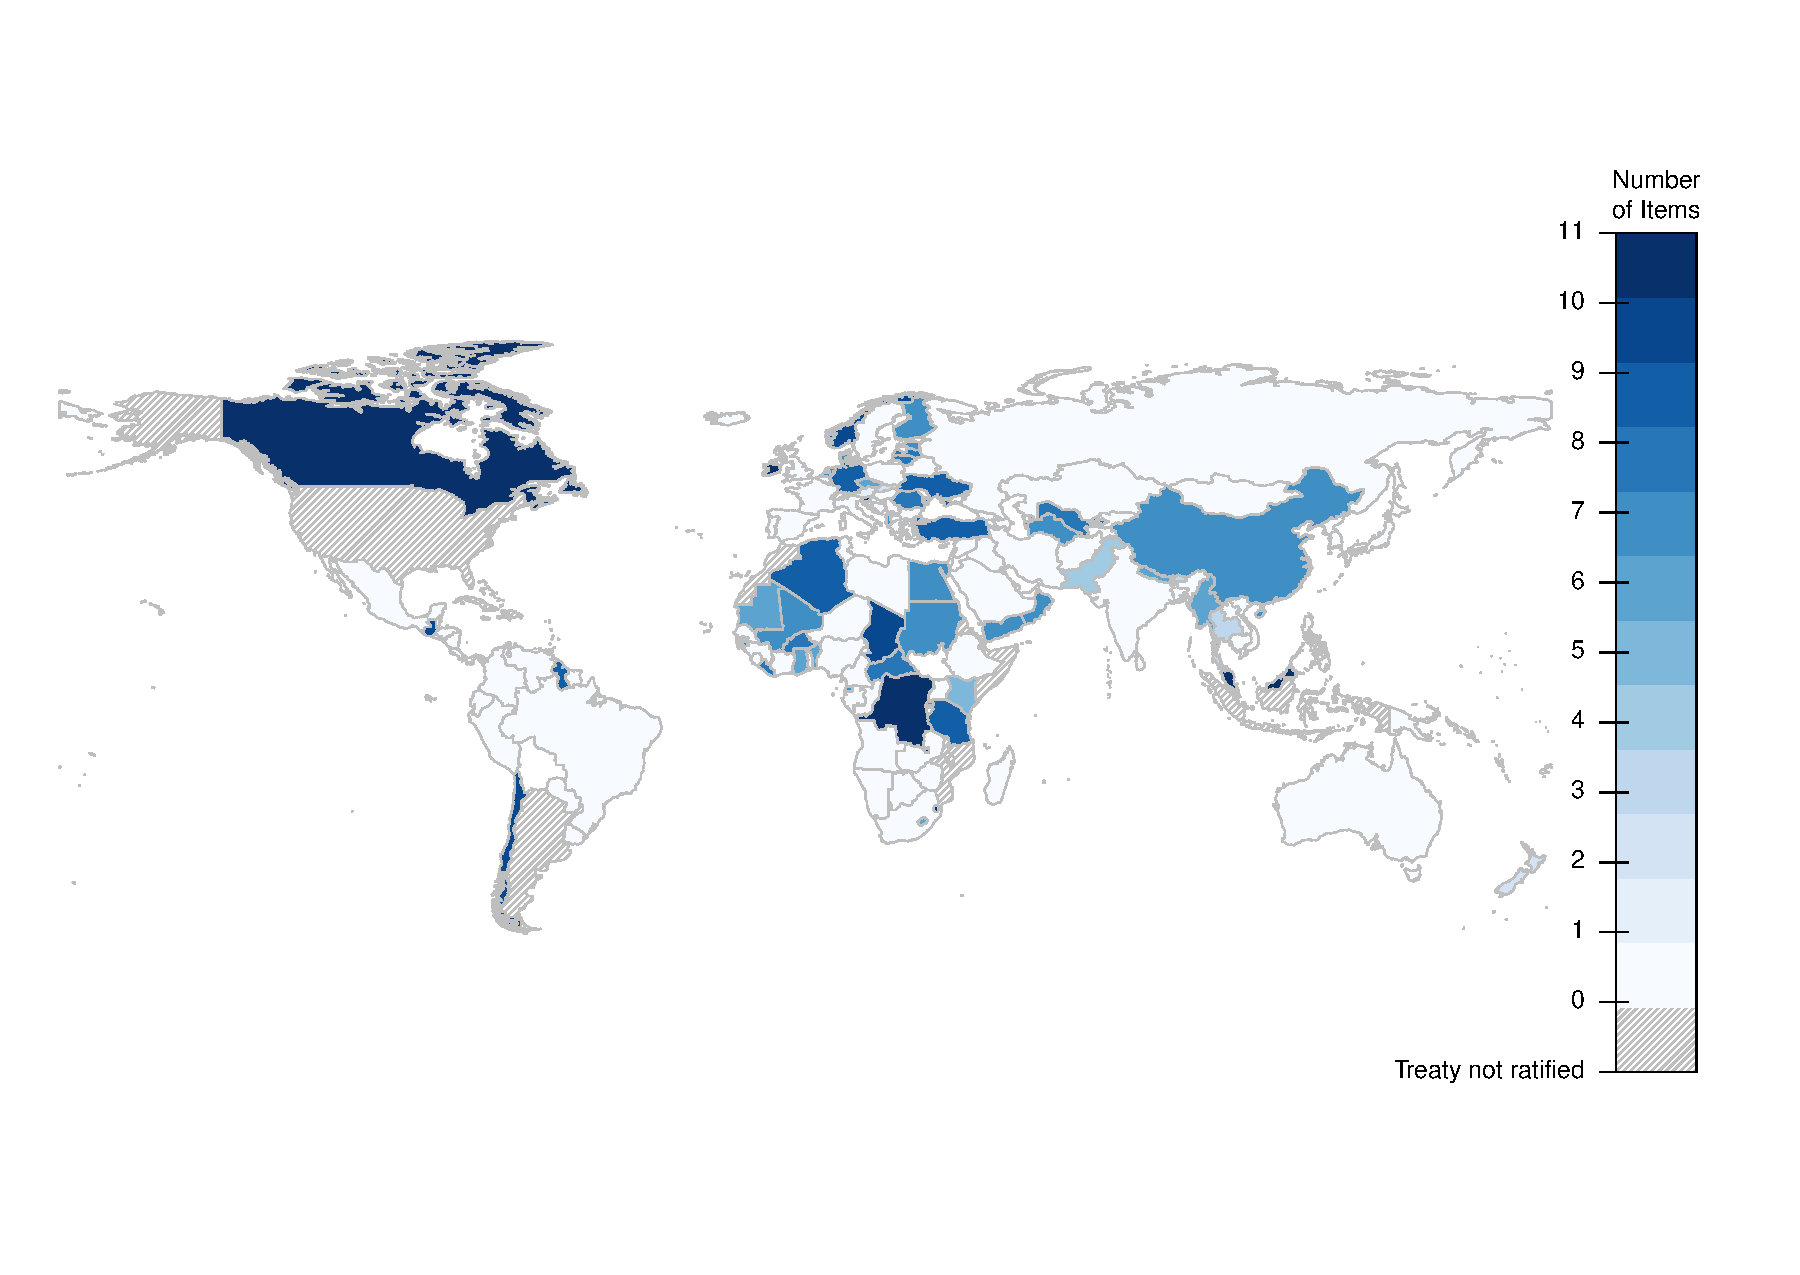
\includegraphics[width=.95\linewidth]{../fig/implementation_art11_map2010.pdf}
\caption{Number of items implemented of Art. 11 by 2010. Source: Downloaded
from http://apps.who.int/fctc/implementation/database}
\end{figure}

\begin{figure}[H]
\centering
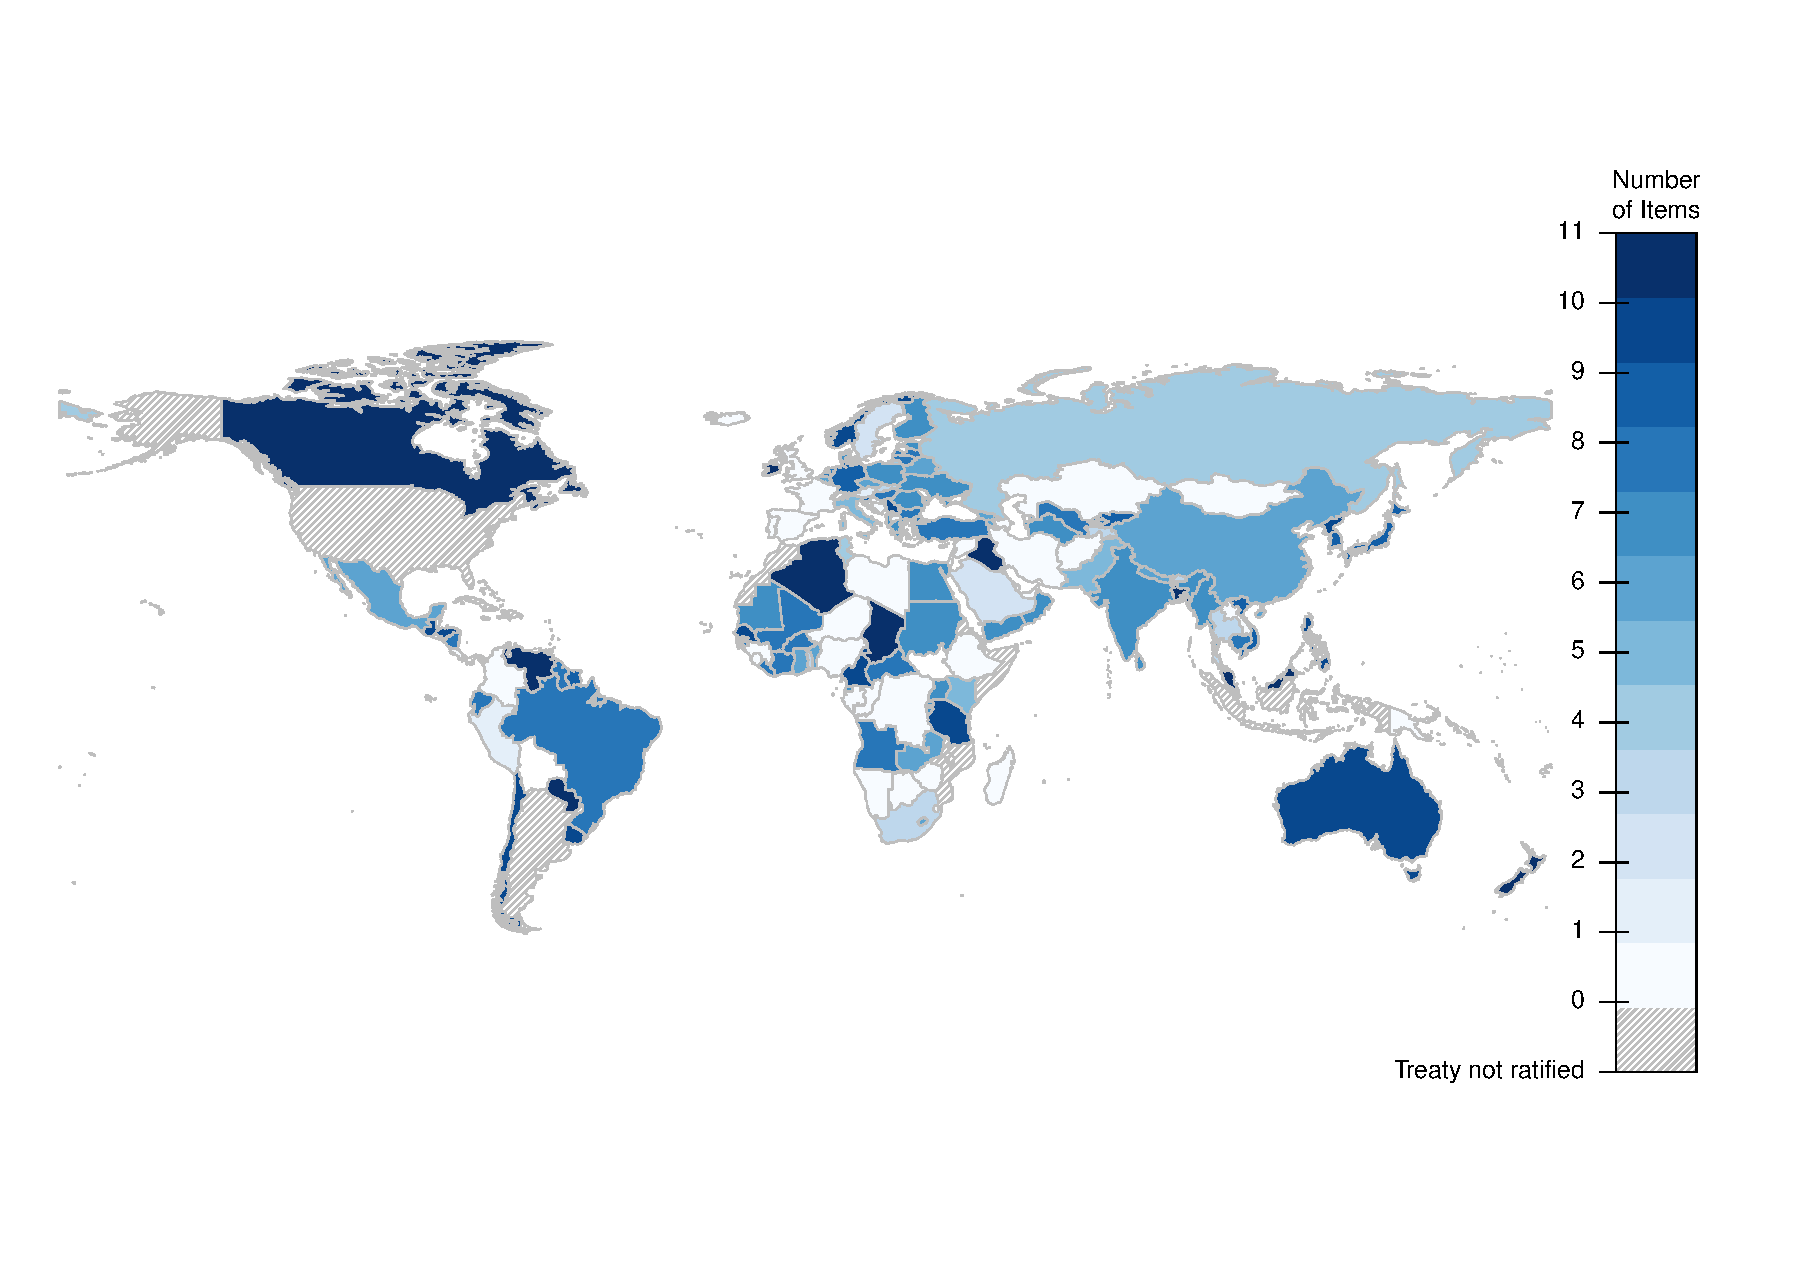
\includegraphics[width=.95\linewidth]{../fig/implementation_art11_map2012.pdf}
\caption{Number of items implemented of Art. 11 by 2012. Source: Downloaded
from http://apps.who.int/fctc/implementation/database}
\end{figure}

\end{landscape}

\end{document}